\documentclass[a4paper,12pt]{classes/fancy}
\usepackage{circuitikz}
\usepackage{graphicx}
\graphicspath{{./images/}}
\usepackage[table]{xcolor}
\usepackage{multicol}
\usepackage{pdflscape}
\usepackage{adjustbox}
\usepackage{wrapfig}
\usepackage{pdfpages}
\usepackage{physics}
\usepackage[version=4]{mhchem}
\newcommand{\Depth}{3}
\newcommand{\Height}{3}
\newcommand{\Width}{3}
\usepackage{pgfplots}
\usetikzlibrary{mindmap}
\usetikzlibrary{shadings,shapes.geometric,calc, patterns, angles, quotes, arrows.meta, shapes, decorations.pathmorphing, decorations.shapes, decorations.text, decorations.markings,shadows}
\tikzstyle directed=[postaction={decorate,decoration={markings, % arrows on the field lines
		mark=at position .1 with {\arrowreversed[scale=1.5]{stealth}},
		mark=at position .9 with {\arrowreversed[scale=1.5]{stealth}}}}]
\tikzstyle tangent=[postaction={decorate,decoration={markings, % Tangent to the field line
		mark=at position .7 with {\draw[ultra thick,stealth-,green!60!black,solid](-12pt,0)--(12pt,0)node[above]{$\vec{B}$};}}}]
\tikzstyle fLines=[thick,dashed,directed,tangent]
\tikzset{
	arrow/.style={-{Triangle[length=5mm,width=2mm]}}
}
\tikzset{
	mypath/.style={
		postaction=decorate,
		decoration={markings,
			mark=at position #1 with {\coordinate (x);\arrow{>}}},
		thick},
	>=stealth
}
\pgfdeclareverticalshading{heat}{100bp}{%
	color(0bp)=(white);   color(25bp)=(white); color(30bp)=(cyan!50); 
	color(70bp)=(orange!70); color(75bp)=(white);  color(100bp)=(white)}
\usetikzlibrary{patterns,fillbetween}
\pgfplotsset{width=8cm,compat=newest}
\def\wall{ \fill
	[fill=black!50] (1,-.5) rectangle (2,.5);
	\pattern [pattern=bricks] (1,-.5) rectangle (2,.5);
	\draw
	[line width=1pt] (1cm+.5pt,-.5) -- ++(0,1); }
\begin{document}
%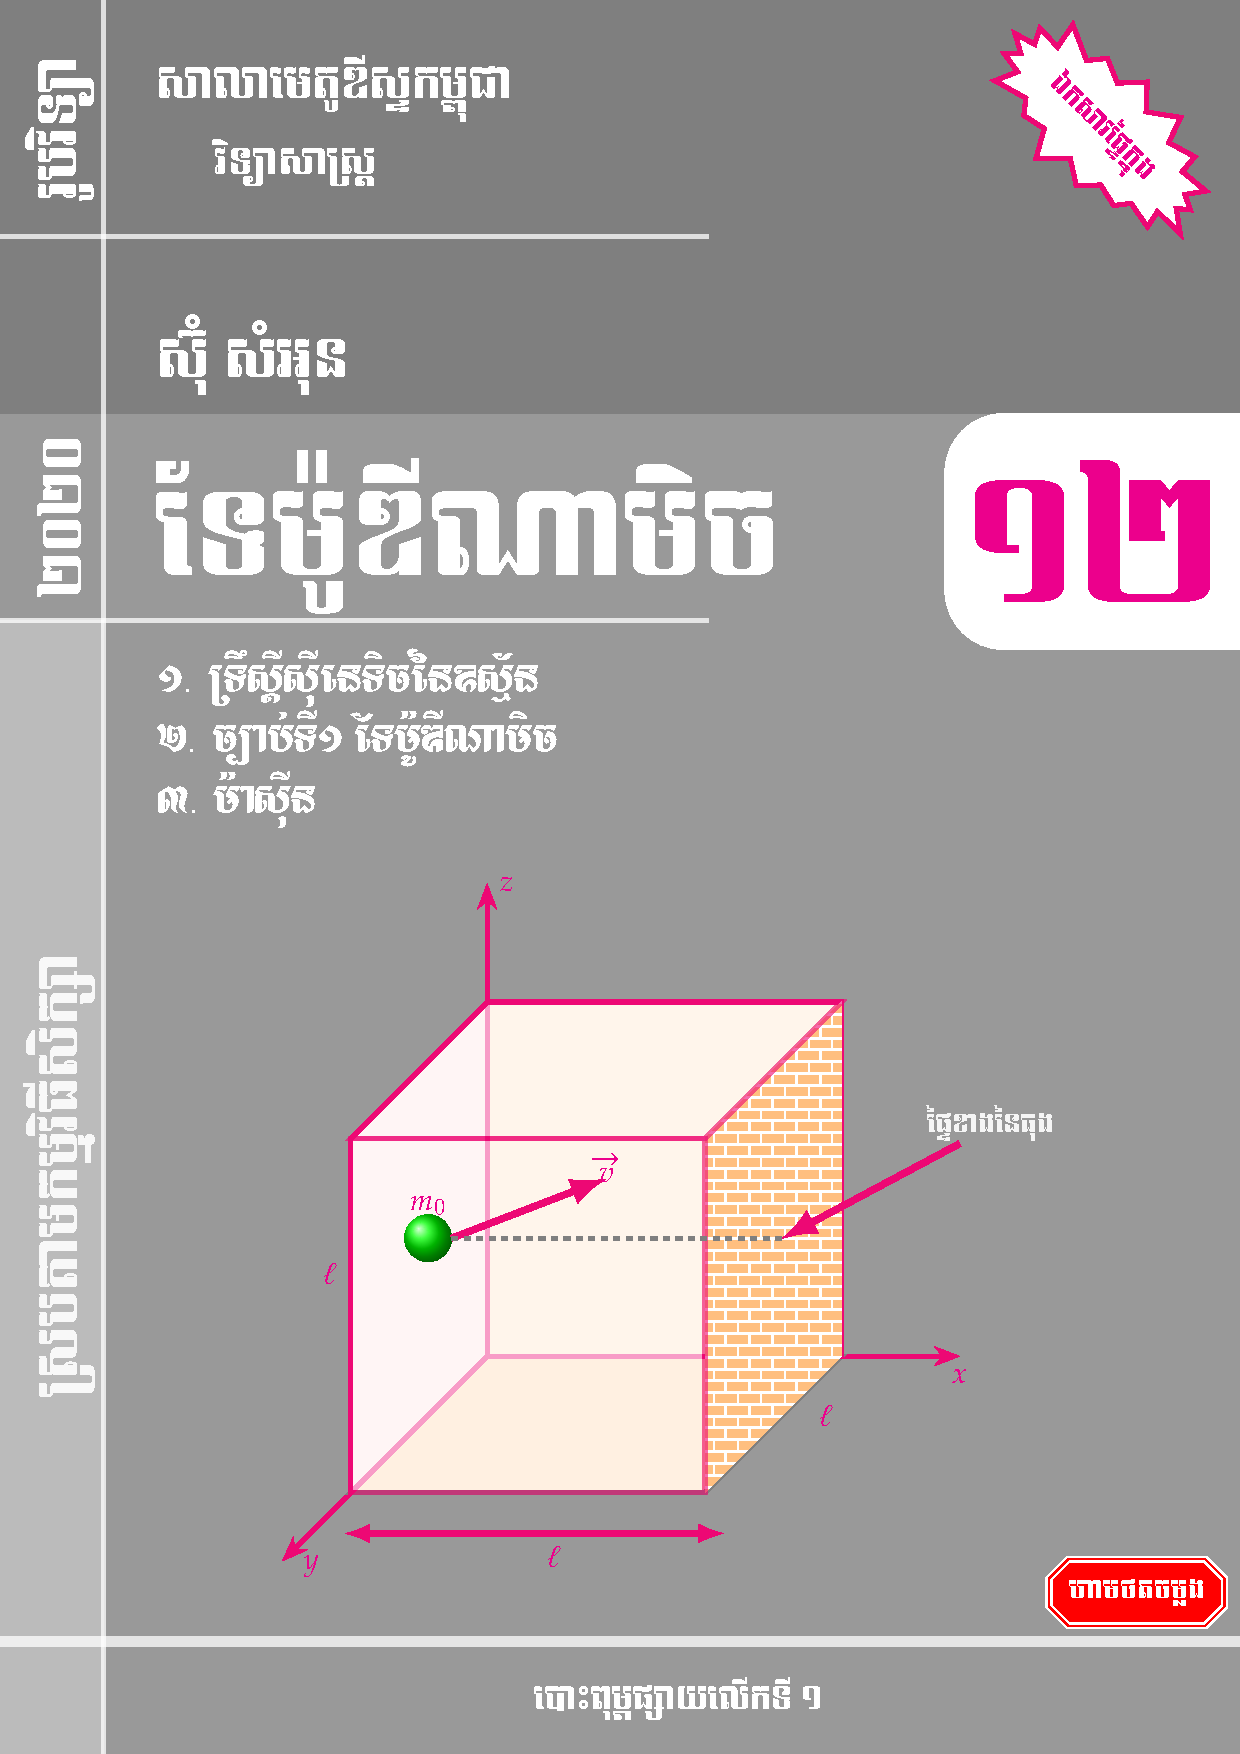
\includepdf{covers/front-cover.pdf}
\frontmatter
\pagenumbering{alpkh}
%\chapter*{សេចក្ដីថ្លែងអំណរគុណ}
\addcontentsline{toc}{chapter}{សេចក្ដីថ្លែងអំណរគុណ}
ខ្ញុំសូមថ្លែងអំណរគុណយ៉ាងជ្រាលជ្រៅដល់មាតាបិតារបស់ខ្ញុំគឺ លោកឪពុក \emph{ឯក~សុភាព} និង អ្នកម្ដាយ \emph{ទុំ~សាហេង} ដែលបានផ្ដល់អ្វីគ្រប់យ៉ាងដល់រូបខ្ញុំ។ ខ្ញុំសូមថ្លែងអំណរគុណដល់ បងប្រុស \emph{ម៉េង~ហុីម} និង បងស្រី \emph{កុយ~ធាវី} ដែលទំនុកបម្រុង ផ្ដល់ដំបូន្មាន និង ការជម្រុញលើកទឹកចិត្ត។ សូមផ្ញើរសេចក្ដីថ្លែងអំណរគុណដល់បងប្អូនខ្ញុំជាច្រើនអ្នកទៀត។
\\[1em]
ជាថ្មីម្ដងទៀតខ្ញុំសូមរំលឹកគុណដល់លោកគ្រូ អ្នកគ្រូរបស់ខ្ញុំដែលបាន បង្ហាត់ពត់លត់ដំខាងផ្នែកបញ្ញាស្មារតី និងវិជ្ជាជីវៈ។\\ បន្ថែមលើនេះខ្ញុំសូមថ្លែងអំណរគុណដល់មិត្តភ័ក្ដិ និងសិស្សានុសិស្សដែលបានផ្ដល់ជាកំលាំងចិត្តដល់រូបខ្ញុំ។
%\chapter*{អារម្ភកថា}
\addcontentsline{toc}{chapter}{អារម្ភកថា}
កថាខណ្ឌនេះពិពណ៌នាអំពីដំណើរដងទងនៃការចាប់កំណើតឡើងនៃសៀវភៅនេះ។ ដំបូងឡើយវាគ្រាន់តែជាកម្រងលំហាត់សម្រាប់ឲ្យសិស្សអនុវត្តន៏បន្ថែមលើការសិក្សាម៉ោងរដ្ធតែប៉ុណ្ណោះ។ ដោយពេលវេលាមានរយៈពេលខ្លី ការដាក់ឧទាហរណ៏ និងលំហាត់គំរូពុំសូវបានច្រើនជាហេតុបណ្ដាលអោយខ្ញុំកើតគំនិតសរសេរចម្លើយដើម្បីអោយសិស្សអាន និងអនុវត្តន៏ដោយខ្លួនឯង។
\\[1em]
សៀវភៅនេះបែងចែកជាបួនផ្នែករួមមាន មេរៀនសង្ខេបអមដោយឧទាហរណ៏គំរូ កម្រងលំហាត់បញ្ចប់មេរៀន ចម្លើយលំហាត់ និង សេចក្ដីបន្ថែម។ នៅផ្នែកមេរៀនសង្ខេបយើងមាន ការរំលឹកខ្លី និយមន័យ លក្ខណៈ និងទ្រឹស្ដីបទ។ ឧទាហរណ៏គំរូសម្រាប់និយមន័យនីមួយៗ ក៏ត្រូវបានរួមបញ្ចូលនៅផ្នែកនេះដែរ។ សម្រាប់សម្រាយបញ្ជាក់ លក្ខណៈ និងទ្រីស្ដីបទសំខាន់អ្នកអានរកមើលនៅផ្នែកបន្ថែមដែលបានដាក់នៅជំពូកចុងក្រោយគេបង្អស់នៃសៀវភៅ។ នៅផ្នែកកម្រងលំហាត់បញ្ចប់មេរៀន យើងមានតែលំហាត់សុទ្ធដែលត្រូវបានរៀបចំតាមខ្លឹមសារមេរៀន និងតាមលំដាប់កើននៃភាពលំបាក។ បន្ទាប់ពីផ្នែកនេះគឺជាចម្លើយលើកម្រងលំហាត់។ រីឯផ្នែកចុងក្រោយ ជាសេចក្ដីបន្ថែម ដែលភាគច្រើនដកស្រង់ចេញពីមេរៀនថ្នាក់ក្រោម។ អ្នកអានគួរផ្ដោតការយកចិត្តទុកលើផ្នែកនេះជាចំបង។ ផ្នែកនេះគួរតែអានមុនគេដើម្បីបង្កភាពងាយស្រួលក្នុងការអានផ្នែកផ្សេងៗទៀត។
\\[1em]
បញ្ជាក់ជួនដល់អ្នកអានសៀវភៅនេះឲ្យបានជ្រាបថា វាគឺជាស្នារដៃដំបូងរបស់អ្នកនិពន្ធ។ សៀវភៅនេះត្រូវបានបង្កើតឡើងដោយមនុស្សតែម្នាក់ប៉ុណ្ណោះ។ ជាងនេះទៅទៀតវាពុំទាន់បានឆ្លងកាត់ការត្រួតពិនិត្យទាំងផ្នែកបច្ចេកទេស និងអក្ខរាវិរុទ នៅឡើយទេ។ បើប្រិយមិត្តរកឃើញកំហុសឆ្គងណាមួយ សូមជួនដំណឹងដល់អ្នកសរសេរសៀវភៅដោយការផ្ញើរសារជាអក្សរ ឬ រូបភាពមកកាន់ប្រអប់សារអេឡិចត្រូនិច ដែលមានអាស័យដ្ឋាន \textcolor{magenta}{\itshape bunnybookauthor@gmail.com} បើមិនអញ្ចឹងទេអ្នកអាចជួបពិភាក្សាផ្ទាល់បើអាចធ្វើទៅបាន។
\\[1em]
ទាក់ទិននឹងការធ្វើអាជីវកម្មលើសៀវភៅនេះ អ្នកនិពន្ធរក្សាសិទ្ធិកម្មសិទ្ធិបញ្ញាដោយមិនអនុញ្ញាតអោយធ្វើការបោះពុម្ភ ថតចំលង ឬចែកចាយដោយគ្មានការអនុញ្ញាតឡើយ។ ចំពោះកំណាត់សៀវភៅនេះជាឯកសារអេឡិចត្រូនិច អ្នកអាចទាញយកមកអាន និងប្រើប្រាស់ផ្ទាល់ខ្លួនបានដោយមិនគិតថ្លៃតាមរយៈដំណរ\\ \textcolor{magenta}{\itshape bunnybookshelf.blogspot.com/p/conic.html}~។
\clearpage
\tableofcontents
\addcontentsline{toc}{chapter}{\contentsname}
\mainmatter
\pagenumbering{khmer}
\chapter{ទំហំវុិចទ័រ និងទំហំស្កាលែ}
\section{ទំហំវុិចទ័រ}
\subsection{ទំហំវិុចទ័រ}
\begin{definition}
	\emph{{\kml ទំហំវិុចទ័រៈ}} ជាទំហំដែលសំដែងជាតម្លៃពីជគណិត ហើយអាស្រ័យនឹង ទិស ទិសដៅ។ វុិចទ័រមួយជាអង្គត់ដែលមានទិសដៅ ភ្ជាប់ពីរចំណុចផ្សេងគ្នា ដែលចំណុចំណុចមួយជាគល់ ឬចំណុចចាប់ និងមួយទៀតជាចុងនៃវុិចទ័រ។
\end{definition}
\begin{example}
	ទំហំវិុចទ័ររួមមានៈ កម្លាំង ល្បឿន សំទុះទំនាញដី ដែនម៉ាញេទិច។ ល។ យើងអាចលើកយកវុិចទ័រ $\overrightarrow{OA}$ មកសិក្សាៈ
	\begin{multicols}{2}
		\begin{itemize}
			\item [$-$] ចំណុចចាប់ ឬគល់ៈ ត្រង់ $O$
			\item [$-$] ទិសៈ ស្ថិតលើបន្ទាត់ $OA$
			\item [$-$] ទិសដៅពី $O$ ទៅ $A$(សម្គាល់ដោយព្រួញ)
			\item [$-$] អាំងតង់សុីតេ ឬម៉ូឌុលៈ $\abs{\overrightarrow{OA}}$
		\end{itemize}
		\begin{figure}[H]
			\centering
			\begin{tikzpicture}[scale=1]
				\begin{scope}
					\coordinate (O) at (0,0);
					\coordinate (A) at (3,2);
					\draw [->] (O) -- (A);
					\coordinate [label=below:$O$] (O) at (O);
					\coordinate [label=above:$A$] (A) at (A);
					\draw (O) node {$\bullet$};
					\draw (1.2,1.5) node {$\overrightarrow{OA}$};
				\end{scope}
			\end{tikzpicture}
			\caption{វុិចទ័រ}
		\end{figure}
	\end{multicols}
\end{example}
\subsection{វុិចទ័រពីរស្មើគ្នា}
\begin{definition}
	\emph{{\kml វុិចទ័រពីរស្មើគ្នាៈ}} កាលណាវុិចទ័រទាំងពីរនោះមានប្រវែងស្មើគ្នា និងមានទិសដៅដូចគ្នា។
\end{definition}
\begin{example}
	ចូរពិនិត្យមើលវិុចទ័រ $\overrightarrow{A}$ និង $\overrightarrow{B}$ ដូចរូបខាងក្រោម។ យើងឃើញថាវុិចទ័រទាំងពីរនេះមានម៉ូឌុល ឬប្រវែងស្មើគ្នា និងមានទិសដៅដូចគ្នា។
	\begin{figure}[H]
		\centering
		\begin{tikzpicture}
			\begin{scope}
				\draw[->] (.1,-.8) --(6,-.8);
				\draw[->] (.5,-1.2) --(.5,2.5);
				\coordinate (O) at (0,0);
				\coordinate (A) at (3,2);
				\coordinate (B) at (2,0);
				\coordinate (C) at (5,2);
				\draw [->] (O) -- (A);
				\draw [->] (B) -- (C);
				\draw (1.2,1.5) node {$\overrightarrow{A}$};
				\draw (3.2,1.5) node {$\overrightarrow{B}$};
				\coordinate [label=below:$O$] (O) at (0.2,-.8);
				\coordinate [label=left:$y$] (y) at (0.5,2.2);
				\coordinate [label=below:$x$] (x) at (6,-.8);
			\end{scope}
		\end{tikzpicture}
		\caption{វុិចទ័រពីរស្មើគ្នា}
	\end{figure}
	ដូចនេះ វុិចទ័រ $\overrightarrow{A}$ ស្មើនឹង $\overrightarrow{B}$ ឬវុិចទ័រទាំងពីរនេះសមភាពគ្នា ទោះបីវាចេញពីគល់ផ្សេងគ្នាក៏ដោយ។ 
	\begin{align*}
		\text{គេសរសេរៈ}\quad :&\quad \overrightarrow{A}=\overrightarrow{B}\\
		\text{នាំឲ្យ}​\quad :&\quad \abs{\overrightarrow{A}}=\abs{\overrightarrow{B}}\quad \text{ឬ}\quad A=B
	\end{align*}
\end{example}
\subsection{ផលបូកវុិចទ័រ}
\begin{enumerate}[m]
	\item \emph{\kml ផលបូកវុិចទ័រពីរមានទិស និងទិសដៅដូចគ្នា}
	\begin{multicols}{2}
			\quad គេមានវុិចទ័រពីរ $\overrightarrow{A}$ និង $\overrightarrow{B}$ ដូចរូបខាងស្តាំ។\\
		យើងបានវិុចទ័រផ្គួបនៃវុិចទ័រ $\overrightarrow{A}$ និង $\overrightarrow{B}$ គឺ $\fbox{$\overrightarrow{C}=\overrightarrow{A}+\overrightarrow{B}$}$
		\begin{figure}[H]
			\centering
			\begin{tikzpicture}
			\begin{scope}[very thick, every node/.style={sloped,allow upside down}]
			\coordinate (O) at (0,2);
			\coordinate (A) at (3,2);
			\coordinate (B) at (1,1);
			\coordinate (C) at (2.5,1);
			\coordinate (D) at (5.5,0);
			\draw [->] (O) -- (A);
			\draw [->] (B) -- (C);
			\draw [->] (0,0) -- (D);
			\draw [arrows = {-Latex[width=6.5pt, length=6.5pt]}] (3.8,0) -- (4,0);
			\draw (1.2,2.4) node {$\overrightarrow{A}$};
			\draw (2,1.4) node {$\overrightarrow{B}$};
			\draw (2,.5) node {$\overrightarrow{A}$};
			\draw (4.5,.5) node {$\overrightarrow{B}$};
			\draw [->] (0,-.5) -- (5.5,-.5);
			\draw (5.7,-.5) node {$\overrightarrow{C}$};
			\end{scope}
			\end{tikzpicture}
			\caption{ផលបូកវុិចទ័រពីរមានទិស និងទិសដៅដូចគ្នា}
		\end{figure}
	\end{multicols}
	ក្នុងករណីដែលយើងចង់រកម៉ូឌុលនៃវុិច $\overrightarrow{C}$ យើងត្រូវលើកអង្គទាំងពីរជាការេ
	\begin{align*}
		\text{យើងបាន}\quad :&\quad \overrightarrow{C^{2}} =\left(\overrightarrow{A}+\overrightarrow{B}\right)^{2}=\overrightarrow{A^{2}} + 2\overrightarrow{A}\overrightarrow{B}+\overrightarrow{B^{2}}=\overrightarrow{A^{2}} + 2AB\cos\left(\overrightarrow{A},\overrightarrow{B}\right) +\overrightarrow{B^{2}}\\
		\text{ដោយ}\quad :&\quad \overrightarrow{C^{2}}=C^{2},~\overrightarrow{A^{2}}=A^{2},~\overrightarrow{B^{2}}=B^{2},~\left(\overrightarrow{A},\overrightarrow{B}\right)=0\\
		\text{យើងបាន}\quad :&\quad C^{2}=A^{2}+2AB+B^{2}=\left(A+B\right)^{2}\\
		\text{នាំឲ្យ}\quad :&\quad C=\sqrt{\left(A+B\right)^{2}}=A+B
	\end{align*}
	\begin{generality}
		អាំងតង់សុីតេវុិចទ័រផ្គួបដែលមានទិសស្របគ្នា និងទិសដៅដូចគ្នាស្មើនឹងផលបូកអាំងតង់សុីតេនៃវុិចទ័រផ្គុំទាំងអស់។
	\end{generality}
	\item \emph{\kml ផលបូកវុិចទ័រពីរមានទិសដូចគ្នា និងទិសដៅផ្ទុយគ្នា}
	\begin{multicols}{2}
		គេមានវុិចទ័រពីរ $\overrightarrow{A}$ និង $\overrightarrow{B}$ ដូចរូបខាងស្តាំ។ គេបានវុិចទ័រ $\overrightarrow{C}=\overrightarrow{A}+\left(-\overrightarrow{B}\right)=\overrightarrow{A}-\overrightarrow{B}\Rightarrow\fbox{$C=A-B$}$\\
		\begin{figure}[H]
			\centering
			\begin{tikzpicture}
			\begin{scope}
			\coordinate (O) at (0,0);
			\coordinate (A) at (3,2);
			\coordinate (B) at (2,0);
			\coordinate (C) at (3.5,1);
			\coordinate (D) at (3.5,1);
			\coordinate (E) at (5,2);
			\draw [->] (O) -- (A);
			\draw [<-] (B) -- (C);
			\draw[->, dashed] (D) -- (E);
			\draw (1.2,1.5) node {$\overrightarrow{A}$};
			\draw (3.7,1.8) node {$\overrightarrow{B}$};
			\draw (3.2,.5) node {$-\overrightarrow{B}$};
			\end{scope}
			\end{tikzpicture}
			\caption{វុិចទ័រពីរមានទិសដូចគ្នា និងទិសដៅផ្ទុយគ្នា}
		\end{figure}
	\end{multicols}
	\begin{multicols}{2}
		ដើម្បីសង់វុិចទ័រផ្គួប $\overrightarrow{C}$ យើងរំកិលវុិចទ័រ $\overrightarrow{B}$ ដោយរក្សាទិសរបស់វាទៅដាក់លើទិសនៃវុិចទ័រ $\overrightarrow{A}$ ដោយដាក់គល់នៃវុិចទ័រ $\overrightarrow{B}$ លើចុងស្លាបព្រួញនៃវុិចទ័រ $\overrightarrow{A}$។
		\begin{figure}[H]
			\centering
			\begin{tikzpicture}
			\begin{scope}
			\coordinate (O) at (0,0);
			\coordinate (A) at (3,2);
			\coordinate (B) at (1,0);
			\coordinate (C) at (2.5,1);
			\coordinate (D) at (2.5,1);
			\coordinate (E) at (3.5,1.7);
			\draw [->] (O) -- (A);
			\draw [->] (B) -- (C);
			\draw[<-] (D) -- (E);
			\draw (1.2,1.5) node {$\overrightarrow{A}$};
			\draw (3.2,1) node {$\overrightarrow{B}$};
			\draw (2,0) node {$\overrightarrow{C}$};
			\end{scope}
			\end{tikzpicture}
			\caption{\DS ផលបូកវុិចទ័រពីរមានទិសដូចគ្នា និងទិសដៅផ្ទុយគ្នា}
		\end{figure}
	\end{multicols}	
	\begin{remark}
		ទិសដៅនៃវុិចទ័រផ្គួបគឺដូចនឹងទិសដៅនៃវុិចទ័រដែលមានអាំងតង់សុីតេធំជាងគេ។
	\end{remark}
	\item \emph{\kml ផលបូកវុិចទ័រពីរមានទិសបង្កើតបានមុំ $\theta$}
		\begin{multicols}{2}
			\quad គេមានវុិចទ័រពីរ $\overrightarrow{A}$ និង $\overrightarrow{B}$ ដែលផ្គុំគ្នាបានមុំ $\theta$ ដូចរូបខាងស្តាំ។ យើងបានវុិចទ័រផ្គួបនៃវុិចទ័រ $\overrightarrow{A}$ និង $\overrightarrow{B}$ គឺតាងដោយ $\overrightarrow{C}=\overrightarrow{A}+\overrightarrow{B}$
			\begin{figure}[H]
				\centering
				\begin{tikzpicture}
				\begin{scope}
				\coordinate (O) at (0,0);
				\coordinate (A) at (2,2);
				\coordinate (B) at (2,0);
				\coordinate (C) at (4,2);
				\draw [->] (O) -- (A);
				\draw [->] (O) -- (B);
				\draw [->] (O) -- (C);
				\draw [dashed] (2,2) --(4,2) -- (2,0);
				\coordinate[label=above:$\overrightarrow{A}$] (A) at (A);
				\coordinate[label=below:$\overrightarrow{B}$] (B) at (B);
				\coordinate[label=above:$\overrightarrow{C}$] (C) at (C);
				\pic [draw, -, "$\theta$", angle eccentricity=1.5] {angle = B--O--A};
				\end{scope}
				\end{tikzpicture}
				\caption{ផលបូកវុិចទ័រពីរមានទិសបង្កើតបានមុំ $\theta$}
			\end{figure}
		\end{multicols}
		យើងអាចលើកអង្គទាំងពីរនៃសមីការនេះជាការេ
		\begin{align*}
		\text{យើងបាន}\quad :&\quad \overrightarrow{C^{2}} =\left(\overrightarrow{A}+\overrightarrow{B}\right)^{2}=\overrightarrow{A^{2}} + 2\overrightarrow{A}\overrightarrow{B}+\overrightarrow{B^{2}}=\overrightarrow{A^{2}} + 2AB\cos\left(\overrightarrow{A},\overrightarrow{B}\right) +\overrightarrow{B^{2}}\\
		\text{ដោយ}\quad :&\quad \overrightarrow{C^{2}}=C^{2},~\overrightarrow{A^{2}}=A^{2},~\overrightarrow{B^{2}}=B^{2},~\left(\overrightarrow{A},\overrightarrow{B}\right)=\theta\\
		\text{យើងបាន}\quad :&\quad C^{2}=A^{2}+B^{2} + 2AB\cos\theta\\
		\text{នាំឲ្យ}\quad :&\quad C=\sqrt{A^{2}+B^{2}+2AB\cos\theta}
		\end{align*}
	\begin{remark}
		ដើម្បីសង់វុិចទ័រផ្គួប $\overrightarrow{C}$ ដែល $\overrightarrow{C}=\overrightarrow{A}+\overrightarrow{B}$ យើងត្រូវអនុវត្តតាមវិធានអង្តត់ទ្រូងប្រលេឡូក្រាម។
	\end{remark}
	\item \emph{\kml ផលបូកវុិចទ័រពីរមានទិស និងទិសដៅកែងគ្នា}
	\begin{multicols}{2}
		\quad គេមានវុិចទ័រពីរ $\overrightarrow{A}$ និង $\overrightarrow{B}$ ដែលផ្គុំគ្នាបានមុំ $90^\circ$ ឬមានទិស និងទិសដៅកែងគ្នា ដូចរូបខាងស្តាំ។ យើងបានវុិចទ័រផ្គួបនៃវុិចទ័រ $\overrightarrow{A}$ និង $\overrightarrow{B}$ គឺតាងដោយ $\overrightarrow{C}=\overrightarrow{A}+\overrightarrow{B}$
		\begin{figure}[H]
			\centering
			\begin{tikzpicture}
			\begin{scope}
			\coordinate (O) at (0,0);
			\coordinate (A) at (2,0);
			\coordinate (B) at (0,2);
			\coordinate (C) at (2,2);
			\draw [->] (O) -- (A);
			\draw [->] (O) -- (B);
			\draw [->] (O) -- (C);
			\draw [dashed] (0,2) --(2,2) -- (2,0);
			\coordinate[label=below:$\overrightarrow{A}$] (A) at (A);
			\coordinate[label=left:$\overrightarrow{B}$] (B) at (B);
			\coordinate[label=above:$\overrightarrow{C}$] (C) at (C);
			\pic [draw, -, "$\alpha$", angle eccentricity=1.5] {angle = A--O--C};
			\end{scope}
			\end{tikzpicture}
			\caption{\DS ផលបូកវុិចទ័រពីរមានទិស និងទិសដៅកែងគ្នា}
		\end{figure}
	\end{multicols}
	យើងអាចលើកអង្គទាំងពីរនៃសមីការនេះជាការេ
	\begin{align*}
		\text{យើងបាន}\quad :&\quad \overrightarrow{C^{2}} =\left(\overrightarrow{A}+\overrightarrow{B}\right)^{2}=\overrightarrow{A^{2}} + 2\overrightarrow{A}\overrightarrow{B}+\overrightarrow{B^{2}}=\overrightarrow{A^{2}} + 2AB\cos\left(\overrightarrow{A},\overrightarrow{B}\right) +\overrightarrow{B^{2}}\\
		\text{ដោយ}\quad :&\quad \overrightarrow{C^{2}}=C^{2},~\overrightarrow{A^{2}}=A^{2},~\overrightarrow{B^{2}}=B^{2},~\left(\overrightarrow{A},\overrightarrow{B}\right)=90^\circ\\
		\text{យើងបាន}\quad :&\quad C^{2}=A^{2}+B^{2}\\
		\text{នាំឲ្យ}\quad :&\quad C=\sqrt{A^{2}+B^{2}}
	\end{align*}
\end{enumerate}
\section{ទំហំស្កាលែ}
\begin{definition}
	\emph{\kml ទំហំស្កាលែៈ} គឺជាបរិមាណចំនួន ឬទំហំក្នុងខ្នាតសមស្របមួយដែលគ្មានទិសដៅ។ នៅក្នុងរូបវិទ្យាទំហំដែលមិនទាក់ទងនឹងទិសដៅ(ទំហំស្កាលែ) មានដូចជាៈ សីតុណ្ហភាព សម្ពាធ ថាមពល កម្មន្ត ម៉ាស រយៈពេល។ ល។
\end{definition}
\section{កូអរដោនេនៃវិុចទ័រ}
	\begin{multicols}{2}
		ឧបមាថាយើងមានត្រីកោណកែង $ABC$ ដូចបង្ហាញក្នុងរូបខាងស្តាំ ។
		\begin{equation*}
			\sin\theta=\frac{\text{ជ្រុងឈម}}{\text{អុីប៉ូតេនុស}},\quad \cos\theta=\frac{\text{ជ្រុងជាប់}}{\text{អុីប៉ូតេនុស}},\quad \tan\theta=\frac{\text{ជ្រុងឈម}}{\text{ជ្រុងជាប់}}
		\end{equation*}
		\begin{figure}[H]
			\centering
			\begin{tikzpicture}
				\centering 
				\begin{scope}
				\large
				\coordinate (C) at (0,0);
				\coordinate (A) at (3,0);
				\coordinate (B) at (3,2);
				\draw (C) -- (A) -- (B) -- cycle;
				\pic [draw, -, "$\theta$", angle eccentricity=1.5] {angle = A--C--B};
				\draw (A) -- ++ (0, .3cm) -- ++ (-.3cm, 0) -- ++ (0, -.3cm);
				\coordinate[label=below:$A$] (A) at (A);
				\coordinate[label=above:$B$] (B) at (B);
				\coordinate[label=below:$C$] (C) at (C);
				\coordinate[label=below:{\text{ជ្រុងជាប់}}] (1.5,0) at (1.5,0);
				\coordinate[label=right:{\text{ជ្រុងឈម}}] (3,1) at (3,1);
				\coordinate[label=right:{\text{អុីប៉ូតេនុស}}] (-1,1) at (-1,1);
				\end{scope}
			\end{tikzpicture}
			\caption{ទំនាក់ទំនងក្នុងត្រីកោណមាត្រ}
		\end{figure}
	\end{multicols}
	ទំនាក់ទំនង់រវាង $\sin\theta$ និង $\cos\theta$ គឺ
	\begin{align*}
		\tan\theta=\frac{\sin\theta}{\cos\theta} \quad \text{និង}\quad \sin^{2}\theta+\cos^{2}\theta=1
	\end{align*}
	\begin{multicols}{2}
		គេមានវុិចទ័រ $\overrightarrow{A}$ ស្តិតក្នុងប្លង់ $xy$ និងបង្កើតបានមុំ $\theta$ ជាមួយអ័ក្ស $Ox$ ដូចរូប។\\ យើងចំណោលកែងវុិចទ័រ $\overrightarrow{A}$ លើអ័ក្ស $Ox$ និង $Oy$ យើងបានធាតុរបស់វា{\en(Components of Vectors)}គឺ $\overrightarrow{A_{x}}$ និង $\overrightarrow{A_{y}}$។ តាមលក្ខណៈនៃវុិចទ័រយើងបានៈ $\overrightarrow{A}=\overrightarrow{A_{x}}+\overrightarrow{A_{y}}$
		\begin{figure}[H]
			\centering
			\begin{tikzpicture}
			\begin{scope}
			\coordinate (O) at (0,0);
			\coordinate (x) at (3,0);
			\coordinate (y) at (0,3);
			\coordinate (A) at (2,2);
			\draw [->] (O) -- (x);
			\draw [->] (O) -- (y);
			\draw [->] (O) -- (A);
			\draw [dashed] (0,2) --(2,2) -- (2,0);
			\coordinate[label=below:$x$] (x) at (x);
			\coordinate[label=left:$y$] (y) at (y);
			\coordinate[label=above:$\overrightarrow{A}$] (A) at (A);
			\coordinate[label=below:$\overrightarrow{A_{x}}$] (2,0) at (2,0);
			\coordinate[label=left:$\overrightarrow{A_{y}}$] (0,2) at (0,2);
			\coordinate[label=below:$O$] (0,0) at (0,0);
			\pic [draw, -, "$\theta$", angle eccentricity=1.5] {angle = x--O--A};
			\end{scope}
			\end{tikzpicture}
			\caption{ផលបូកវុិចទ័រពីរមានទិស និងទិសដៅកែងគ្នា}
		\end{figure}
	\end{multicols}
	\begin{proof}
		\begin{align*}
			\text{ដែល}\quad :&\quad A_{x}=A\cos\theta \quad\text{និង}\quad A_{y}=A\sin\theta\\
				\text{យើងបាន}\quad :&\quad \overrightarrow{A^{2}} =\left(\overrightarrow{A_{x}}+\overrightarrow{A_{y}}\right)^{2}=\overrightarrow{A^{2}_{x}} + 2\overrightarrow{A_{x}}\overrightarrow{A_{y}}+\overrightarrow{A_{y}^{2}}=\overrightarrow{A៌_{x}^{2}} + 2A_{x}A_{y}\cos\left(\overrightarrow{A_{x}},\overrightarrow{A_{y}}\right) +\overrightarrow{A_{y}^{2}}\\
			\text{ដោយ}\quad :&\quad \overrightarrow{A^{2}}=A^{2},~\overrightarrow{A_{x}^{2}}=A_{x}^{2},~\overrightarrow{A_{y}^{2}}=A_{y}^{2},~\left(\overrightarrow{A_{x}},\overrightarrow{A_{y}}\right)=90^\circ\\
			\text{យើងបាន}\quad :&\quad A^{2}=A_{x}^{2}+A_{y}^{2}\\
			\text{នាំឲ្យ}\quad :&\quad A=\sqrt{A_{x}^{2}+A_{y}^{2}}
		\end{align*}
	\end{proof}
\section{លំហាត់}
\begin{enumerate}[m]
	\item ចូរពោលទ្រឹស្តីសុីនេទិចនៃឧស្ម័ន។
	\item ចូរសរសេរសមីការភាពនៃឧស្ម័នបរិសុទ្ធ។
	\item ចូរសរសេររូបមន្តថាមពលសុីនេទិចមធ្យមនៃម៉ូលេគុលឧស្ម័ននីមួយៗ។
	\item ចូរសរសេររូបមន្តថាមពលសុីនេទិចសរុបនៃម៉ូលេគុលឧស្ម័ន។
	\item ចូរសរសេររូបមន្តល្បឿនប្ញសការេនៃការេល្បឿនមធ្យមម៉ូលេគុលឧស្ម័ន។
	\item ក្នុងធុងបិទជិតមួយមានផ្ទុកឧស្ម័នអុកសុីសែន $\left(\ce{O2}\right)~2mol$។\\
	គណនាចំនួនម៉ូលេគុលរបស់ឧស្ម័នអុកសុីសែននេះ បើចំនួនអាវ៉ូកាដ្រូ $N_{A}=6.022\times10^{23}$ ម៉ូលេគុល$/mol$។
	\item ក្នុងធុងបិទជិតមួយមានឧស្ម័នអុីដ្រូសែន $\left(\ce{H2}\right)~0.2mol$ និងមានម៉ាសម៉ូល $2.0g/mol$។\\
	បើគេដឹងថា ចំនួនអាវ៉ូកាដ្រូ $N_{A}=6.022\times10^{23}$ម៉ូលេគុល$/mol$។
	\begin{enumerate}[k]
		\item គណនាចំនួនម៉ូលេគុលអុីដ្រូសែនក្នុងធុងនេះ។
		\item គណនាម៉ាសសរុបរបស់ឧស្ម័នអុីដ្រូសែន។
	\end{enumerate}
	\item ក្នុងធុងបិទជិតមួយមានឧស្ម័ន $0.25mol$ និងមានម៉ាសសរុប $7.0g$។\\
	បើគេដឹងថា ចំនួនអាវ៉ូកាដ្រូ $N_{A}=6.022\times10^{23}$ម៉ូលេគុល$/mol$។
	\begin{enumerate}[k]
		\item គណនាចំនួនម៉ូលេគុលសរុបរបស់ឧស្ម័នក្នុងធុងនេះ។
		\item តើឧស្ម័ននេះជាឧស្ម័នអ្វី?
	\end{enumerate}
	\item ក្នុងធុងបិទជិតមួយមានឧស្ម័នពេញ មានម៉ាសសរុប $64.0g$ និងមានចំនួនម៉ូលេគុលសរុបគឺ $12.044\times10^{23}$ម៉ូលេគុល។\\
	បើគេដឹងថា ចំនួនអាវ៉ូកាដ្រូ $N_{A}=6.022\times10^{23}$ម៉ូលេគុល$/mol$។
	\begin{enumerate}[k]
		\item គណនាចំនួនម៉ូលរបស់ឧស្ម័នក្នុងធុងនេះ។
		\item តើឧស្ម័ននេះជាឧស្ម័នអ្វី?
	\end{enumerate}
	\item ក្នុងធុងបិទជិតមួយមានផ្ទុក ឧស្ម័ន $\ce{H2}$ ពេញមានម៉ាសសរុប $1.0g$។ ដោយឧស្ម័ននេះមានម៉ាសម៉ូល $2.0g/mol$ និងចំនួនអាវ៉ូកាដ្រូ $N_{A}=6.022\times10^{23}$ម៉ូលេគុល$/mol$។
	\begin{enumerate}[k]
		\item គណនាចំនួនម៉ូលេគុលសរុបរបស់ឧស្ម័នក្នុងធុងនេះ។
		\item គណនាចំនួនម៉ូលរបស់ឧស្ម័ន $\ce{H2}$។
	\end{enumerate}
	\item ផង់នីមួយៗមានម៉ាស $m_{0}$ និងផ្លាស់ទីដោយល្បឿន $v$ តាមបណ្តោយអ័ក្ស $\overrightarrow{ox}$។ គេដឹងថាក្នុងផ្ទៃ $1mm^{2}$ និងក្នុង $1s$ មានផង់ចំនួន $10^{15}$ ទៅទង្គិចនឹងផ្ទៃនោះ។
	ចូររកសម្ពាធរបស់ផង់លើផ្ទៃប៉ះ។\\
	គេឲ្យ $m_{0}=9.1\times10^{-31}kg$ និង $v=8\times10^{7}m/s$។ គេសន្មត ទង្គិចរវាងផង់ និងផ្ទៃប៉ះជាទង្គិចស្ទក់។
	\item គេបាញ់ផង់ឲ្យផ្លាស់ទីតាមបណ្តោយអ័ក្ស $\overrightarrow{ox}$ ដែលកែងនឹងផ្ទៃរបស់អេក្រង់មួយ។ គេដឹងថា ផង់នីមួយៗមានម៉ាស $m_{0}$ និងល្បឿន $v_{0}$។ គេដឹងថាក្នុង $1.25mm^{2}$ ផ្ទៃរបស់អេក្រង់មានផង់ចំនួន $4\times10^{14}$ ទៅទង្គិចរៀងរាល់វិនាទី។ \\គេសន្មតថា ទង្គិចនោះជាទង្គិចស្ទក់។ គណនាល្បឿនរបស់ផង់ដែលផ្លាស់ទីតាមអ័ក្ស $\overrightarrow{ox}$។\\ បើគេដឹងថា សម្ពាធដែលកើតឡើងដោយសារការទង្គិចរបស់ផង់លើផ្ទៃអេក្រង់គឺ $P=3.64\times10^{-3}N/m^{2}\\~m_{0}=9.1\times10^{-31}kg$។
	\item ផង់នីមួយមានម៉ាស $m_{0}$ នឹងផ្លាស់ទីដោយល្បឿន $v$ តាមបណ្តោយអ័ក្ស $\overrightarrow{ox}$។ គេដឹងថាក្នុងផ្ទៃ $2mm^{2}$ និងក្នុងមួយវិនាទីមានផង់ចំនួន $2\times10^{15}$ ទៅទង្គិចនឹងផ្ទៃនោះ។ គេឲ្យៈ $m_{0}=9.1\times10^{-31}kg$ និង $v=5\times10^{7}m/s$។ គេសន្មតថា ទង្គិចរវាងផង់ និងផ្ទៃប៉ះជាទង្គិចស្ទក់។
	\begin{enumerate}[k,2]
		\item គណនាកម្លាំងសរុបដែលផង់មានអំពើលើផ្ទៃប៉ះ។
		\item គណនាសម្ពាធសរុបរបស់ផង់លើផ្ទៃប៉ះ។
	\end{enumerate}
	\item ប្រូតុងមួយមានម៉ាស $m_{p}=1.67\times10^{-27}kg$ ផ្លាស់ទីដោយល្បឿន $v$ តាមបណ្តោយអ័ក្ស $\overrightarrow{ox}$ ក្នុងមាឌមួយមានរាងជាគូបដែលទ្រនុងនីមួយៗមានរង្វាស់ $3mm$ ប្រូតុងផ្លាស់ពីផ្ទៃម្ខាងទៀតក្នុង $2ns$។ គេសន្មត់ថា ទង្គិចរវាងប្រូតុង និងផ្ទៃខាងនៃគូបជាទង្គិចស្ទក់។
	\begin{enumerate}[k]
		\item រកល្បឿនដើមប្រូតុង នៅខណៈវាចាប់ផ្តើមចេញពីផ្ទៃខាងនៃគូប។
		\item រកសម្ពាធរបស់ប្រូតុងលើផ្ទៃខាងនៃគូប។
		\item គេដឹងថាក្នុងរយៈពេល $2ns$ មានចំនួនប្រូតុង $2\times10^{6}$ ទៅទង្គិចនឹងផ្ទៃខាងនៃគូប។ រកសម្ពាធសរុបរបស់ប្រូតុងលើផ្ទៃខាងនៃគូប។
	\end{enumerate}
	\item អេឡិចត្រុងមួយមានម៉ាស $m_{e}=9.1\times10^{-31}kg$ ផ្លាស់ទីដោយល្បឿន $v$ តាមបណ្តោយអ័ក្ស $\overrightarrow{ox}$ ក្នុងមាឌមួយមានរាងជាគូបដែលទ្រនុងនីមួយៗមានរង្វាស់ $5mm$ ប្រូតុងផ្លាស់ពីផ្ទៃម្ខាងទៀតក្នុង $25ns$។ \\គេសន្មត់ថា ទង្គិចរវាងប្រូតុង និងផ្ទៃខាងនៃគូបជាទង្គិចស្ទក់។
	\begin{enumerate}[k]
		\item រកល្បឿនដើមអេឡិចត្រុង នៅខណៈវាចាប់ផ្តើមចេញពីផ្ទៃខាងនៃគូប។
		\item រកសម្ពាធរបស់អេឡិចត្រុងលើផ្ទៃខាងនៃគូប។
		\item គេដឹងថាក្នុងរយៈពេល $25ns$ មានចំនួនអេឡិចត្រុង $2\times10^{10}$ ទៅទង្គិចនឹងផ្ទៃខាងនៃគូប។\\ រកសម្ពាធសរុបរបស់អេឡិចត្រុងមានលើផ្ទៃខាងនៃគូប។
	\end{enumerate}
	\item អេឡិចត្រុងមួយមានម៉ាស $m_{e}=9.1\times10^{-31}kg$ ផ្លាស់ទីដោយល្បឿន $v$ តាមបណ្តោយអ័ក្ស $\overrightarrow{ox}$ ក្នុងមាឌមួយមានរាងជាគូបដែលទ្រនុងនីមួយៗមានរង្វាស់ $2mm$ ប្រូតុងផ្លាស់ពីផ្ទៃម្ខាងទៀតក្នុង $25ns$។ គេសន្មត់ថា ទង្គិចរវាងប្រូតុង និងផ្ទៃខាងនៃគូបជាទង្គិចខ្ទាត។
	\begin{enumerate}[k]
		\item រកល្បឿនដើមអេឡិចត្រុង នៅខណៈវាចាប់ផ្តើមចេញពីផ្ទៃខាងនៃគូប។
		\item រកសម្ពាធរបស់អេឡិចត្រុងលើផ្ទៃខាងនៃគូប។
		\item គេដឹងថាក្នុងរយៈពេល $25ns$ មានចំនួនអេឡិចត្រុង $25\times10^{6}$ ទៅទង្គិចនឹងផ្ទៃខាងនៃគូប។\\ រកសម្ពាធសរុបរបស់អេឡិចត្រុងមានលើផ្ទៃខាងនៃគូប។
	\end{enumerate}
	\item អាតូមអុីដ្រូសែនមួយមានម៉ាស $m$ ផ្លាស់ទីដោយល្បឿន $v=1500km/s$ តាមបណ្តោយអ័ក្ស $\overrightarrow{ox}$ ក្នុងមាឌមួយមានរាងគូបដែលទ្រនុងនីមួយមានរង្វាស់ $3mm$។ អុីដ្រូសែន ផ្លាស់ទីពីផ្ទៃម្ខាងទៅម្ខាងទៀត។ គេសន្មតថាសន្មត់ថា ទង្គិចរវាងអុីដ្រូសែន និងផ្ទៃខាងនៃគូបជាទង្គិចខ្នាត។
	\begin{enumerate}[k]
		\item រករយៈពេលដែលអាតូមអុីដ្រូសែនទៅប៉ះនឹងផ្ទៃម្ខាងទៀតនៃគូប។
		\item គេដឹងថាក្នុងរយៈពេល $2ns$ មានចំនួនអាតូមអុីដ្រូសែន $2\times10^{6}$ ទៅទង្គិចនឹងផ្ទៃខាងនៃគូបហើយផ្ទៃខាងរងនៅសម្ពាធសរុប $27.83\times10^{-2}N/m^{2}$។ រកម៉ាសអាតូមអុីដ្រូសែនមួយ។
	\end{enumerate}
	\item ឧស្ម័នបរិសុទ្ធមួយមានមាឌ $V=100cm^{3}$ ស្ថិតក្រោមសម្ពាធ $2.00\times10^{5}Pa$ នៅសីតុណ្ហភាព $20^\circ C$។\\ តើឧស្ម័ននោះមានប៉ុន្មានម៉ូល? $\left(R=8.31J/mol\cdot K\right)$
	\item ឧស្ម័នបរិសុទ្ធមួយមាន $n=0.08\times10^{-1}mol$ មានសម្ពាធ $P=5.00\times10^{5}Pa$ នៅសីតុណ្ហភាព $60^\circ C$។\\ តើឧស្ម័ននោះមានមាឌប៉ុន្មាន?
	\item នៅសីតុណ្ហភាព $293K$ និងសម្ពាធ $5atm$ មេតាន $1kmol$ មានម៉ាស $16.0kg$។ \\គណនាម៉ាសមាឌនៃមេតានក្នុងលក្ខខណ្ឌខាងលើ។
	\item នៅក្នុងបំពង់បិទជិតដែលមានមាឌ $20mL$ នៅសីតុណ្ហភាពកំណត់មួយយ៉ាងទាបមានតំណក់នីត្រូសែនរាវមានម៉ាស $50mg$។ គណនាសម្ពាធនីត្រូសែននៅក្នុងបំពង់នោះ កាលណាបំពង់នោះមានសីតុណ្ហភាព $300K$ ដោយសន្មតថានីត្រូសែននេះជាឧស្ម័នបរិសុទ្ធ។ គេឲ្យៈ $R=8.31J/mol\cdot K$។
	\item ធុងមួយមានផ្ទុកអេល្យូម $2.00mol$ នៅសីតុណ្ហភាព $27^\circ C$។ គេសន្មតថាអេល្យូមជាឧស្ម័នបរិសុទ្ធ។
	\begin{enumerate}[k]
		\item គណនាតម្លៃមធ្យមនៃថាមពលសុីនេទិចរបស់ម៉ូលេគុលនីមួយៗ
		\item គណនាថាមពលសុីនេទិចសរុបរបស់ម៉ូលេគុលទាំងអស់។\\
		គេឲ្យៈ $k_{B}=1.38\times10^{-23}J/K,~R=8.31J/mol\cdot K$។
	\end{enumerate}
	\item នៅក្នុងធុងមួយដែលមានមាឌ $2.00mL$ មានឧស្ម័នដែលមានម៉ាស $50mg$ និងសម្ពាធ $100kPa$។\\ ម៉ាសរបស់មូលេគុលនៃឧស្ម័ននីមួយៗគឺ $8.0\times10^{-26}kg$។
	\begin{enumerate}[k]
		\item រកចំនួនម៉ូលេគុលនៃឧស្ម័ននោះ។
		\item រកតម្លៃមធ្យមនៃថាមពលសុីនេទិចរបស់ម៉ូលេគុលនីមួយៗ។ គេឲ្យៈ $k=1.38\times10^{-23}J/K$
	\end{enumerate}
	\item ចូរគណនាប្ញសការេនៃការេល្បឿនមធ្យមរបស់អាតូមអេល្យូមនៅសីតុណ្ហភាព $20.0^\circ C$។ \\ម៉ាសម៉ូលអេល្យូមគឺ $4.00\times10^{-3}kg/mol$។ គេឲ្យៈ $R=8.31J/mol\cdot K$។
	\item រកប្ញសការេនៃការេល្បឿនមធ្យមរបស់ម៉ូលេគុលអុកសុីសែននៅសីតុណ្ហភាព $200^\circ C$។ \\ម៉ាសម៉ូលអុកសុីសែន $32\times10^{-3}kg/mol$ និង $R=8.31J/mol\cdot K$។
	\item \begin{enumerate}[k]
		\item គណនាម៉ាសម៉ូលេគុលនៃអុីដ្រូសែន។ គេឲ្យម៉ាសម៉ូលគឺ $M=2.00\times10^{-3}kg/mol$ \\និងចំនួនអាវ៉ូកាដ្រូ $N_{A}=6.02\times10^{23}/mol$។
		\item គណនាតម្លៃប្ញសការេនៃការេល្បឿនមធ្យមរបស់ឧស្ម័នអុីដ្រូសែននៅសីតុណ្ហភាព $100^\circ C$។
		\item គណនាតម្លៃមធ្យមនៃថាមពលសុីនេទិចរបស់ម៉ូលេគុលនៃឧស្ម័នអុីដ្រូសែននីមួយៗនៅសីតុណ្ហភាព $100^\circ C$។\\ គេឲ្យៈ $k=1.38\times10^{-23}$។
	\end{enumerate}
	\item ដោយប្រើតម្លៃលេខ $1,3,7$ និង $8$ ចូរបង្ហាញថា ប្ញសការេនៃការេល្បឿនមធ្យម $v_{rms}$ \\ខុសគ្នាពីតម្លៃមធ្យម $v_{av}$ របស់វា។
	\item ចូរកំណត់រកល្បឿន $v_{rms}$ របស់ម៉ូលេគុលឧស្ម័នអុកសុីសែន $\left(O_{2}\right)$ និងអាសូត $\left(N_2\right)$ ក្នុងបន្ទប់មួយដែលមានសីតុណ្ហភាព $20^\circ C$។
	\item \begin{enumerate}[k]
		\item បង្ហាញថាល្បឿន $v_{rms}$ នៃឧស្ម័នបរិសុទ្ធ អាចសរសេរជាទម្រង់មួយទៀតគឺ $v_{rms}=\sqrt{\frac{3P}{\rho}}$ ដែល $\rho$ ជាដង់សុីតេ ឬហៅថាម៉ាសមាឌ ហើយ $P$ ជាសម្ពាធ។
		\item ល្បឿន $v_{rms}$ របស់ម៉ូលេគុលឧស្ម័នមួយប្រភេទស្មើ $450m/s$។\\ ប្រសិនបើវាស្ថិតនៅសម្ពាធបរិយាកាស តើដងសុីតេរបស់ឧស្ម័ននោះស្មើប៉ុន្មាន?
	\end{enumerate}
	\item កែវបាឡុងមួយចំណុះ $1L$ មានអុកសុីសែនជាឧស្ម័នបរិសុទ្ធដែលមានសីតុណ្ហភាព $27^\circ C$ ក្រោមសម្ពាធ $2atm$។\\
	គណនាម៉ាសអុកសុីសែន។ គេឲ្យៈ $O=16$
	\item គេមានខ្យល់មានមាឌ $1m^3$ នៅសីតុណ្ហភាព $18^\circ C$ ក្នុងសម្ពាធបរិយាកាស $P_{1}=1atm$ ទៅបណ្ណែននៅសីតុណ្ហភាពដដែល តែក្នុងសម្ពាធបរិយាកាស $P_{2}=3.5atm$។ គណនាមាឌស្រេចនៃខ្យល់។
	\item ដបមួយផ្ទុកឧស្ម័នមានសម្ពាធ $P_{0}=1.0atm$ នៅសីតុណ្ហភាព $17^\circ C$។\\
	តើគេត្រូវកម្តៅឪ្យឧស្ម័ននេះដល់សីតុណ្ហភាពប៉ុន្មាន ដើម្បីសម្ពាធកើនឡើងដល់ $1.5atm$?
	\item គេយកបំពង់អុកសុីសែនមានចំណុះ $20L$ ក្រោមសម្ពាធ $P_{1}=200atm$ នៅសីតុណ្ហភាព $20^\circ C$ ទៅដាក់ក្នុងបាឡុង កៅស៊ូស្តើងមួយ។\\ គណនាមាឌបាឡុង បើឧស្ម័នក្នុងបាឡុងមានសម្ពាធ $P_{2}=1atm$ និងសីតុណ្ហភាព $9^\circ C$។
	\item \begin{enumerate}[k]
		\item ចូរគណនាល្បឿនប្រសិទ្ធ $\left(v_{rms}\right)$ នៃម៉ួលេគុលឧស្ម័ននីត្រូសែននៅសីតុណ្ហភាព $20^\circ C$។
		\item គណនាសីតុណ្ហភាព ប្រសិនបើល្បឿនប្រសិទ្ធ $\left(v_{rms}\right)$ ថយចុះពាក់កណ្តាល។
		\item គណនាសីតុណ្ហភាព ប្រសិនបើល្បឿនប្រសិទ្ធ $\left(v_{rms}\right)$ កើនឡើងពីរដងវិញ។
	\end{enumerate}
	\item មួយ ម៉ូលេគុលឧស្ម័ននីដ្រូសែនផ្សំឡើងពីអាតូមនីដ្រូសែនពីរ។គណនាម៉ាសម៉ូលេគុលនីត្រូសែន។\\ ម៉ាសម៉ូលនីដ្រូសែនគឺ $M=28kg/kmol$ គេឲ្យ $N_{A}=6.02\times10^{23}$ ម៉ូលេគុល$/mol$
	\item គណនាមាឌឧស្ម័នអុកសុីសែន $3.2g$ ដែលផ្ទុកក្នុងធុងនៅសម្ពាធ $76cmHg$ និងសីតុណ្ហភាព $27^\circ C$។
	\item រកល្បឿនប្រសិទ្ធ $v_{rms}$ នៃម៉ូលេគុលអាសូតដោយម៉ាសម៉ូល $M=28g/mol$ នៅ $300K$។ គេឲ្យៈ $R=8.31J/mol\cdot K$
	\item គណនាសីតុណ្ហភាពដែលធ្វើឲ្យល្បឿនប្រសិទ្ធនៃម៉ូលេគុលអុីដ្រូសែនស្មើ $331m/s$។ គេឲ្យៈ $M_{H_{2}}=2.0g/mol$។ 
	\item គណនាតម្លៃមធ្យមនៃថាមពលសុីនេទិចនៃម៉ូលេគុលឧស្ម័ននៅសីតុណ្ហភាព $727^\circ C$។ គេឲ្យៈ $R=8.31J/mol\cdot K$ និង $N_{A}=6.02\times10^{23}$ម៉ូលេគុល$/mol$។
	\item រកតម្លៃមធ្យមនៃថាមពលសុីនេទិចរបស់ម៉ូលេគុលឧស្ម័នអុកសុីសែននីមួយៗក្នុងខ្យល់នៅក្នុងបន្ទប់មានសីតុណ្ហភាព $300K$ គិតជាអេឡិចត្រុង-វ៉ុល។ គេឲ្យ $1eV=1.6\times10^{-19}J$ និង $k_{B}=1.38\times10^{-23}J/K$
	\item មួយម៉ូលេគុលនីដ្រូសែននៅពេលស្ថិតនៅលើផ្ទៃដីវាកើតមានល្បឿនប្រសិទ្ធ នៅសីតុណ្ហភាព $0^\circ C$។ ប្រសិនបើវាផ្លាស់ទីឡើងត្រង់ទៅលើដោយគ្មានទង្គិចនឹងម៉ូលេគុលផ្សេងទៀត។ ចូរគណនាកម្ពស់ដែលវាឡើងដល់។ \\គេឲ្យម៉ាសមួយម៉ូលេគុលរបស់នីដ្រូសែន $m=4.65\times10^{-26}kg$ និង $g=10m/s^{2}$។
	\item សុីទែនមួយស្ថិតក្រោមលក្ខខណ្ឌស្តង់ដា {\en (STP)} ផ្ទុកឧស្ម័ននីដ្រូសែន $28.5kg$។
	\begin{enumerate}[k]
		\item ចូរគណនាមាឌរបស់សុីទែន។
		\item ប្រសិនបើគេបន្ថែមនីដ្រូសែន $32.2kg$ ទៀតចូលក្នុងសុីទែនដោយរក្សាសីតុណ្ហភាពនៅដដែល។ \\ចូរគណនាសម្ពាធឧស្ម័ននីដ្រូសែនក្នុងសុីទែន។
	\end{enumerate}
	\item បាច់ម៉ូលេគុលអុីដ្រូសែនត្រូវបានបាញ់លើជញ្ជាំងដោយទិសបង្កើតបានមុំ $55^\circ$ ជាមួយនឹងវុិចទ័រឯកតាផ្ទៃ $\left(\overrightarrow{n}\right)$ របស់ជញ្ជាំង។ ម៉ូលេគុលនីមួយៗនៃឧស្ម័នអុីដ្រូសែនមានល្បឿន $1km/s$ និងម៉ាស $3.3\times10^{-24}kg$។ បាច់អុីដ្រូសែនបានទៅទង្គិចនឹងជញ្ជាំងដែលមានផ្ទៃ $2cm^{2}$ ដោយអត្រា $10^{23}$ ម៉ូលេគុលក្នុងមួយវិនាទី។\\ ដោយសន្មតថាទង្គិចនេះ ជាទង្គិចខ្ទាត ចូរគណនាសម្ពាធដែលមានលើជញ្ជាំង។
	\item គេបាញ់ផង់ឲ្យផ្លាសើទីតាមបណ្តោយអ័ក្ស $\overrightarrow{ox}$ ដែលកែងនឹងផ្ទៃរបស់អេក្រង់មួយ។ គេដឹងថាផង់នីមួយៗមានម៉ាស $m_{0}$ និងមានល្បឿន $v$។ គេដឹងថាក្នុង $1.25mm^{2}$ ផ្ទៃរបស់អេក្រង់មានផង់ $4\times10^{14}$ ទៅទង្គិចរៀងរាល់វិនាទី។\\ គេសន្មត់ថា ទង្គិចនោះជាទង្គិចស្ទក់។
	គណនាល្បឿនរបស់ផង់ដែលផ្លាស់ទីតាមតាមអ័ក្ស $\overrightarrow{ox}$។ បើគេដឹងថា សម្ពាធដែលកើតឡើងដោយសារការទង្គិចរបស់ផង់លើផ្ទៃរបស់អេក្រង់គឺ $3.64\times10^{-3}N\cdot m^{-2}$ និង $m_{0}=9.1\times10^{-31}kg$។
	\item ផង់នីមួយៗមានម៉ាស $m_{0}$ និងផ្លាស់ទីដោយល្បឿន $v$ តាមបណ្តោយអ័ក្ស $\overrightarrow{ox}$។ គេដឹងថាក្នុងផ្ទៃ $2mm^{2}$ និងក្នុងមួយវិនាទីមានផង់ចំនួន $2\times10^{15}$ ទៅទង្គិចនឹងផ្ទៃនោះ។ គេឲ្យៈ $m_{0}=9.1\times10^{-31}kg$ និង $v=5.0\times10^{15}m/s$។\\
	គេសន្មតថា ទង្គិចរវាងផង់និងផ្ទៃប៉ះជាទង្គិចស្ទក់។
	\begin{enumerate}[k]
		\item គណនាកម្លាំងសរុបដែលផង់មានអំពើលើផ្ទៃប៉ះ។
		\item គណនាសម្ពាធសរុបរបស់ផង់លើផ្ទៃប៉ះ។
	\end{enumerate}
	\item  ប្រូតុងមួយមានម៉ាស $m_{P}=1.67\times10^{-27}kg$ និងផ្លាស់ទីដោយល្បឿនដើម $\overrightarrow{v}_{0}$ តាមបណ្តោយអ័ក្ស $\overrightarrow{ox}$ ក្នុងធុងមួយមានរាងជាគូប។ គេដឹងថាក្នុងផ្ទៃ $4mm^{2}$ និងក្នុងមួយវិនាទីមានប្រូតុងចំនួន $5\times10^{13}$ ទៅទង្គិចនឹងផ្ទៃនោះហើយសម្ពាធរបស់ប្រូតុងលើផ្ទៃប៉ះគឺ $8.35\times10^{-2}Pa$។ គេសន្មតថាទង្គិចរវាងផង់នឹងផ្ទៃប៉ះជាទង្គិចស្ទក់។
	\begin{enumerate}[k]
		\item គណនាកម្លាំងដែលប្រូតុងនីមួយៗមានអំពើលើផ្ទៃប៉ះ។
		\item គណនាល្បឿនប្រូតុងនៅខណៈវាទៅប៉ះនឹងផ្ទៃម្ខាងទៀតនៃគូប។
	\end{enumerate}
	\item អេឡិចត្រុងមួយមានម៉ាស $m_{e}=9.1\times10^{31}kg$ ផ្លាស់ទីដោយល្បឿន $v$ តាមបណ្តោយអ័ក្ស $\overrightarrow{ox}$។ ក្នុងធុងមួយមានរាងជាគូបដែលទ្រនុងនីមួយៗមានរង្វាស់ $l=5mm$។ អេឡិចត្រុងផ្លាស់ទីពីផ្ទៃម្ខាងទៅផ្ទៃម្ខាងទោក្នុង $25ns$។\\ គេសន្មតថាទង្គិចរវាងអេឡិចត្រុង នឹងផ្ទៃខាងនៃគូបជាទង្គិចស្ទក់។
	\begin{enumerate}[k]
		\item គណនាល្បឿនស្រេចអេឡិចត្រុង នៅខណៈវាទៅប៉ះនឹងផ្ទៃម្ខាងទៀតនៃគូប។
		\item គណនាសម្ពាធរបស់អេឡិចត្រុងមានលើផ្ទៃខាងនៃគូប។
		\item គេដឹងថាក្នុងរយៈពេល $25ns$ មានចំនួនអេឡិចត្រុង $2\times10^{10}$ ទៅទង្គិចនិងផ្ទៃខាងនៃគូប។\\ គណនាសម្ពាធសរុបរបស់អេឡិចត្រុងមានលើផ្ទៃខាងនៃគូប។
	\end{enumerate}
	\item សម្ពាធនៃឧស្ម័ននៅក្នុងធុងមួយមានមាឌ $250mL$ ស្ថិតនៅក្រោមសម្ពាធ $125kPa$ និងថាមពលសុីនេទិចមធ្យមនៃភាគល្អិតនីមួយៗគឺ $1.875\times10^{-21}J$។
	\begin{enumerate}[k]
		\item គណនាចំនួនភាគល្អិតនៃឧស្ម័ននៅក្នុងធុង។
		\item គណនាចំនួនម៉ូលនៃ ឧស្ម័ននៅក្នុងធុង។ គេឲ្យៈ $N_{A}=6.022\times10^{23}$ម៉ូលេគុល$/mol$
	\end{enumerate}
\item ក្នុងធុងមួយមានមាឌ $200mL$ មានម៉ូលេគុលសរុប $5\times10^{21}$ ហើយស្ថិតនៅក្រោមសម្ពាធ $250kPa$។\\ ថេរបុលស្មាន់ $k_{B}=1.38\times10^{-23}J/K$ និង ចំនួនអាវ៉ូកាដ្រូ $N_{A}=6.022\times10^{23}$ម៉ូលេគុល$/mol$
\begin{enumerate}[k]
	\item គណនាថាមពលសុីនេទិចមធ្យមនៃភាគល្អិតនីមួយៗ។
	\item គណនាចំនួនម៉ូលនៃ ឧស្ម័ននៅក្នុងធុង។
	\item គណនាសីតុណ្ហភាពនៃឧស្ម័ននៅក្នុងធុង។
\end{enumerate}
\item ឧស្ម័នបរិសុទ្ធមួយមានមាឌ $V=500cm^{3}$ ស្ថិតក្រោមសម្ជាធ $600kPa$ នៅសីតុណ្ហភាព $27^\circ C$។ \\គណនាចំនួនម៉ូលនៃ ឧស្ម័ននោះ។ គេឲ្យថេរសាកលនៃឧស្ម័ន $R=8.31J/mol\cdot K$
\item ឧស្ម័នបរិសុទ្ធមួយមាន $n=0.25mol$ មានសម្ពាធ $P=250kPa$ នៅសីតុណ្ហភាព $57^\circ C$។ \\តើឧស្ម័ននោះមានមាឌប៉ុន្មាន? គេឲ្យថេរសាកលនៃឧស្ម័ន $R=8.31J/mol\cdot K$
\item ធុងមួយមានផ្ទុកឧស្ម័នអេល្យូម $0.5mol$ នៅសីតុណ្ហភាព $27^\circ C$។ គេសន្មតថាអេល្យូមជាឧស្ម័នបរិសុទ្ធ។\\ គេឲ្យៈ $k_{B}=1.38\times10^{-23}J/K$ និង $R=8.31J/mol\cdot K$។
\begin{enumerate}[k]
	\item គណនាតម្លៃមធ្យមនៃថាមពលសុីនេតិចរបស់ម៉ូលេគុលឧស្ម័ននីមួយៗ។
	\item គណនាថាមពលសុីនេទិចសរុបរបស់ម៉ូលេគុលទាំងអស់។
	\item គណនាសម្ពាធឧស្ម័នអេល្យូមក្នុងធុង​ បើធុងមានមាឌ $4.53\times10^{-3}m^{3}$។
\end{enumerate}
\item \begin{enumerate}[k]
	\item គណនាល្បឿនប្រសិទ្ធនៃម៉ូលេគុលអុកសុីសែននៅសុីតុណ្ហភាព $127^\circ C$។ \\ម៉ាសម៉ូលអុកសុីសែនគឺ $32g/mol$ និង $R=8.31J/mol\cdot K$។
	\item គណនាតម្លៃថាមពលសុីនេទិចមធ្យមនៃម៉ូលេគុលឧស្ម័នអុកសុីសែននីមួយៗ នៅសីតុណ្ហភាព $127^\circ C$។ \\គេឲ្យៈ $k_{B}=1.38\times10^{-23}J/K$
\end{enumerate}
\item \begin{enumerate}[k]
	\item គណនាសីតុណ្ហភាពនៃម៉ូលេគុលអុីដ្រូសែនគិតជា $^\circ C$។\\ បើដឹងថា ល្ពៀនប្រសិទ្ធនៃម៉ូលេគុលអុីដ្រូសែន $v_{rms}=1933.78m\cdot s^{-1}$ ម៉ាសម៉ូលអុីដ្រូសែនស្មើនឹង $2.0g/mol$ និងគេឲ្យៈ $R=8.31J/mol\cdot K;~k_{B}=1.38\times10^{-23}J/K$។
	\item គណនាតម្លៃថាមពលសុីនេទិចមធ្យមនៃម៉ូលេគុលអុីដ្រូសែននីមួយៗ នៅសីតុណ្ហភាពនោះ។​
\end{enumerate}
\item ធុងមួយមានមាឌ $V=2.5mL$ មានផ្ទុកឧស្ម័នដែលមានម៉ាស $50mg$ ស្ថិតក្រោមសម្ពាធ $1035kPa$។ \\ម៉ាសរបស់ម៉ូលេគុលនៃឧស្ម័ននីមួយៗគឺ $8\times10^{-26}kg$។
\begin{enumerate}[k]
	\item គណនាចំនួនម៉ូលេគុលសរុបនៃឧស្ម័ននោះ។ គេឲ្យៈ $k_{B}=1.38\times10^{-23}J/K$។
	\item គណនាតម្លៃថាមពលសុីនេទិចមធ្យមនៃម៉ូលេគុលឧស្ម័ននីមួយៗ
	\item គណនាតម្លៃថាមពលសុីនេទិចសរុបរបស់ម៉ូលេគុលក្នុងធុង។
	\item គណនាសីតុណ្ហភាពនៃឧស្ម័នក្នុងធុង។
\end{enumerate}
\item ឧស្ម័នបរិសុទ្ធមួយមានមាឌ $V=125cm^3$ ស្ថិតក្រោមសម្ពាធ $2\times10^{5}Pa$។\\ គណនាសីតុណ្ហភាពនៃឧស្ម័នបរិសុទ្ធនោះ។ បើគេដឹងថាឧស្ម័ននោះមាន $n=9.4\times10^{-3}mol;~R=8.31J/mol\cdot K$។
\item ធុងមួយមានមាឌ $0.025m^{3}$ ផ្ទុកម៉ាស $0.084kg$ នៃឧស្ម័ននីដ្រូសែន $\ce{N2}$ ស្ថិតនៅក្រោមសម្ពាធ $3.17atm$។\\ គណនាសីតុណ្ហភាពនៃឧស្ម័នគិតជាអង្សារសេ$\left(^\circ C\right)$។ គេឲ្យៈ $1atm=1.013\times10^{5}Pa$ ម៉ាសម៉ូល $M=28g/mol$ និង $R=8.31J/mol\cdot K$។
\item ផង់នីមួយៗមានម៉ាស $m_{0}$ និងផ្លាស់ទីដោយល្បឿន $\overrightarrow{v}$ តាមបណ្តោយអ័ក្ស $\overrightarrow{ox}$។ គេដឹងថាក្នុងផ្ទៃ $5mm^2$ និងក្នុងមួយវិនាទីមានផង់ចំនួន $1\times10^{15}$ ទៅទង្គិចនឹងផ្ទៃនោះ។ គណនាសម្ពាធសរុបរបស់ផង់មានលើផ្ទៃប៉ះ។ គេសន្មតថា ទង្គិចរវាងផង់នឹងផ្ទៃប៉ះជាទង្គិចស្ទក់ ហើយម៉ាសផង់នីមួយៗគឺ $m_{0}=9.1\times10^{-31}kg$ និង $v=8\cdot10^{7}m/s$។
\item គណនាចំនួនម៉ូលេគុលសរុបដែលមាននៅក្នុង $500g$ នៃខ្យល់។\\ បើគេដឹងថាក្នុងខ្យល់មានអុកសុីសែន​ $22\%$ និងមានអាសូត $78\%$ ជាម៉ាស។
\item ក្នុងធុងបិទជិតមួយមានមាឌសរុប $16.62dm^3$ មានផ្ទុកឧស្ម័នបរិសុទ្ធពេញស្ថិតក្រោមសម្ពាធ $3\times10^{5}Pa$ និងមានសីតុណ្ហភាព $47^\circ C$។ គេឲ្យថេរឧស្ម័នបរិសុទ្ធ $R=8.31J/mol\cdot K$។ គណនាចំនួនម៉ូលនៃឧស្ម័នបរិសុទ្ធក្នុងធុងនោះ។
\item ឧស្ម័នបរិសុទ្ធមួយមានម៉ាសម៉ូលេគុលនីមួយៗគឺ $8\times10^{-26}kg$ នៅសីតុណ្ហភាព $57^\circ C$។​\\ គេឲ្យៈ $k_{B}=1.38\times10^{-23}J/K$។
\begin{enumerate}[k]
	\item គណនាប្ញសការេនៃការេល្បឿនមធ្យម $v_{rms}$។
	\item គណនាតម្លៃថាមពលសុីនេទិចមធ្យមនៃម៉ូលេគុលឧស្ម័នបរិសុទ្ធនីមួយៗ។
\end{enumerate}
\item \begin{enumerate}
	\item គណនាម៉ាសម៉ូលេគុលនីមួយៗរបស់ឧស្ម័នអុកសុីសែន។\\ បើគេដឹងថាម៉ាសម៉ូលរបស់វាគឺ $32g/mol$ និង $N_{A}=6.022\times10^{23}$ម៉ូលេគុល$/mol$
	\item គណនាល្បឿនប្រសិទ្ធនៃឧស្ម័នអុកសុីសែនស្ថិតនៅសីតុណ្ហភាព $0^\circ C$។
	\item គណនាតម្លៃថាមពលសុីនេទិចមធ្យមនៃម៉ូលេគុលនីមួយៗ របស់ឧស្ម័នអុកសុីសែននៅសីតុណ្ហភាព $0^\circ C$។\\ គេឲ្យៈ $k_{B}=1.38\times10^{-23}J/K$
\end{enumerate}
\item បាឡុងពីរត្រូវបានតភ្ជាប់គ្នាដោយបំពង់មួយមានរ៉ូពីនេបិទជិត។ ដោយបាឡុងទី១ មានផ្ទុកឧស្ម័នដែលមានសម្ពាធ $5atm$ និងមានមាឌ $6L$ ចំណែកបាឡុងទី២នៅទទេមានមាឌ $4L$។\\ គេចាប់ផ្តើមបើករ៉ូពីនេ(បើគេដឹងថាបាឡុងនីមួយៗមានសីតុណ្ហភាពថេរ)។\\ គណនាសម្ពាធរបស់បាឡុងនីមួយៗ ក្រោយពេលគេបើករ៉ូពីនេ។
\item បាឡុងពីរត្រូវបានតភ្ជាប់គ្នាដោយបំពង់មួយមានរ៉ូពីនេបិទជិត។ ដោយបាឡុងទី១ មានផ្ទុកឧស្ម័នដែលមានសម្ពាធ $6atm$ និងមានមាឌ $5L$ ចំណែកបាឡុងទី២ មានផ្ទុកឧស្ម័នដូចគ្នាដែលមានសម្ពាធ $4atm$ និងមានមាឌ $3L$។\\ គេចាប់ផ្តើមបើករ៉ូពីនេ(បើគេដឹងថាបាឡុងនីមួយៗមានសីតុណ្ហភាពថេរ)។\\ គណនាសម្ពាធរបស់បាឡុងនីមួយៗ ក្រោយពេលគេបើករ៉ូពីនេ។
\item កំណត់សីតុណ្ហភាពដើម្បីឲ្យល្បឿនប្រសិទ្ធនៃម៉ូលេគុលឧស្ម័នអាសូតដែលមានម៉ាសម៉ូល $M_{\left(\ce{N2}\right)}=28g/mol$ ស្មើនឹងល្បឿនប្រសិទ្ធនៃម៉ូលេគុលឧស្ម័នអុកសុីសែន ដែលមានម៉ាសម៉ូល $M_{\left(\ce{O2}\right)}=32g/mol$ នៅសីតុណ្ហភាព $47^\circ C$។
\item គូបមួយមានជ្រុង $10.0cm$ ផ្ទុកខ្យល់ដែលមានម៉ាសម៉ូល $28.9g/mol$ នៅសម្ពាធបរិយាកាស និងសីតុណ្ហភាព $300K$។
\begin{enumerate}[k]
	\item គណនាម៉ាស និងទម្ងន់នៃឧស្ម័នក្នុងរូប។
	\item គណនាកម្លាំងដែលមានអំពើលើផ្ទៃខាងនីមួយៗនៃគូប។
	\item តើហេតុអ្វីបានជាសំណាកដ៏តូចល្អិតមួយអាចបង្កើតកម្លាំងដ៏មហិមានេះបាន?
\end{enumerate}
\item \begin{enumerate}[k]
	\item គណនាចំនួនម៉ូលនៃឧស្ម័នបរិសុទ្ធដែលមានមាឌ $1m^{3}$ នៅសីតុណ្ហភាព $20.0^\circ C$ និងសម្ពាធបរិយាកាស។
	\item ក្នុងមួយម៉ូលនៃម៉ូលេគុលខ្យល់មានម៉ាស $28.9g$។ គណនាម៉ាសខ្យល់ក្នុង $1m^{3}$។
\end{enumerate}
\item ឧស្ម័នអុកសុីសែនមួយម៉ូលមានសម្ពាធ $P_{1}$ នៅសីតុណ្ហភាព $27.0^\circ C$។
\begin{enumerate}[k]
	\item បើឧស្ម័នត្រូវបានកម្តៅដោយរក្សាមាឌថេររហូតដល់សម្ពាធកើនឡើងបីដង ចូរគណនាសីតុណ្ហភាពនៃឧស្ម័ន។
	\item បើឧស្ម័នមានសម្ពាធ និងមាឌកើនឡើងពីរដង ចូរគណនាសីតុណ្ហភាពរបស់ឧស្ម័ន។
\end{enumerate}
\item នៅក្រោមផ្ទៃទឹកសមុទ្រជម្រៅ $25.0m$ មានម៉ាសមាឌ $\rho=1025kg/m^{3}$ មានសីតុណ្ហភាព $5^\circ C$។ ពពុះខ្យល់មួយមានមាឌ $1cm^{3}$ ផុសចេញមកលើផ្ទៃទឹកដែលមានសីតុណ្ហភាព $20^\circ C$។\\ គណនាមាឌរបស់ពពុះខ្យល់ពេលរៀបបែកចូលក្នុងខ្យល់។
\item គេដាក់ទឹក $9.0g$ ទៅក្នុងធុងដែលមានចំណុះ $2.0L$ រួចដុតកម្តៅដល់សីតុណ្ហភាព $500^\circ C$។ \\គណនាសម្ពាធក្នុងធុង។
\item សវនដ្ខានមួយមានវិមាត្រ $10.0m\times20.0m\times30.0m$។\\ គណនាចំនួនម៉ូលេគុលខ្យល់នៅក្នុងសវនដ្ខាននោះនៅកម្រិតសីតុណ្ហភាព $20.0^\circ C$ និងសម្ពាធ $101kPa$។
\item \begin{enumerate}[k]
	\item បង្ហាញឲ្យឃើញថា ម៉ាសមាឌឧស្ម័នបរិសុទ្ធដែលមានមាឌ $V$ មានទំនាក់ទំនង់ $\rho =\frac{PM}{RT}$ ដែល $P$ ជាសម្ពាធឧស្ម័ន $M$ ជាម៉ាសម៉ូលឧស្ម័ន $T$ ជាសីតុណ្ហភាពឧស្ម័ន និង $R$ ជាថេរសកលនៃឧស្ម័ន។
	\item គណនាម៉ាសមាឌនៃឧស្ម័នអុកសុីសែននៅសម្ពាធធម្មតា និងសីតុណ្ហភាព $20.0^\circ C$។
\end{enumerate}
\item មាសមានម៉ាសម៉ូល $197g/mol$។
\begin{enumerate}[k]
	\item គណនាចំនួនម៉ូលនៃអាតូមមាសក្នុងគម្រូមាសសុទ្ធ $2.50g$។
	\item គណនាចំនួនអាតូមដែលមានក្នុងគម្រូខាងលើ។
\end{enumerate}
\item គណនាៈ ចំនួនម៉ូល និងចំនួនម៉ូលេគុលក្នុង $1.00cm^{3}$ នៃឧស្ម័នបរិសុទ្ធនៅសម្ពាធ $100Pa$ និងសីតុណ្ហភាព $220K$។
\item គណនាតម្លៃមធ្យមនៃថាមពលសុីនេទិចរបស់ម៉ូលេគុលឧស្ម័នបរិសុទ្ធក្នុងករណីៈ
\begin{enumerate}[1]
	\item \begin{enumerate}[k]
		\item សីតុណ្ហភាព $0.00^\circ C$។
		\item សីតុណ្ហភាព $100^\circ C$។
	\end{enumerate}
	\item គណនាថាមពលសុីនេទិចសរុបក្នុងមួយម៉ូលនៃឧស្ម័នបរិសុទ្ធក្នុងករណីៈ
	\begin{enumerate}[k]
		\item សីតុណ្ហភាព $0.00^\circ C$។
		\item សីតុណ្ហភាព $100^\circ C$។
	\end{enumerate}
\end{enumerate}
\item គណនា​ប្ញសការេនៃការេល្បឿនមធ្យម $v_{rms}$ នៃអាតូមអេល្យូមនៅសីតុណ្ហភាព $1000K$។ \\គេឲ្យម៉ាសម៉ូលអេល្យូម $M=4.00g/mol$
\item គណនាថាមពលសុីនេទិចមធ្យមនៃម៉ូលេគុលនីត្រូសែននៅសីតុណ្ហភាព $1600K$។
\item ឧស្ម័នអុកសុីសែនមួយមានមាឌ $1000cm^{3}$ នៅសីតុណ្ហភាព $40^\circ C$ និងមានសម្ពាធ $1.01\times10^{5}Pa$ បានរីករហូតដល់មាឌរបស់វា $1500cm^{3}$ និងសម្ពាធរបស់វាគឺ $1.06\times10^{5}Pa$។
\begin{enumerate}[k]
	\item គណនាចំនួនម៉ូលនៃឧស្ម័នអុកសុីសែនខាងលើ។
	\item គណនាសីតុណ្ហភាពស្រេចនៃឧស្ម័នគម្រូខាងលើ។
\end{enumerate}
\item ក្នុងប្រព័ន្ធសុញ្ញាកាសខ្ពស់មួយ សម្ពាធដែលអាចវាស់បានស្មើនឹង $1.00\times10^{-10}torr$(ដែល $1torr=133Pa$)។ ឧបមាថា សីតុណ្ហភាពស្មើនឹង $300K$។ គេឲ្យ ថេប៊ុលស្មាន់ $k_{B}=1.38\times10^{-23}J/K$\\
ចូរគណនាចំនួនម៉ូលេគុលក្នុងមាឌមួយស្មើនឹង $1.00cm^{3}$។
\item បរិមាណនៃឧស្ម័នបរិសុទ្ធនៅសីតុណ្ហភាព $10.0^\circ C$ និងសម្ពាធ $100kPa$ ត្រូវបានគេបំពេញទៅក្នុងមាឌ $2.50m^{3}$។ គេឲ្យ ថេរសកលនៃឧស្ម័ន $R=8.31J/mol\cdot K$
\begin{enumerate}[k]
	\item គណនាចំនួនម៉ូលនៃឧស្ម័នដែលបានរៀបរាប់ខាងលើ។
	\item ប្រសិនបើសម្ពាធឡើងដល់ $300kPa$ និងសីតុណ្ហភាពឡើងដល់ $30.0^\circ C$។\\ គណនាមាឌដែលត្រូវយកឧស្ម័នទៅបំពេញ សន្មតថាគ្មានលិចឧស្ម័ន។
\end{enumerate}
\item ប្រសិនបើ ម៉ាស $m=2.1212g$ នៃឧស្ម័នបរិសុទ្ធមួយមានមាឌ $V=1.49L$ ស្ថិតក្នុងលក្ខខណ្ឌដែលមានសីតុណ្ហភាព $t=0^\circ C$ និងសម្ពាធ $P=810.6kPa$ តើវាជាឧស្ម័នអ្វី? គេឲ្យៈ $R=8.31J/mol\cdot K$។
\item បាឡុងរាងស៊វែរមួយមានមាឌ $4000cm^{3}$ ផ្ទុកដោយអេល្យូមនៅសម្ពាធ(ខាងក្នុង) $1.20\times10^{5}Pa$។ គណនាចំនួនម៉ូលនៃអេល្យូមក្នុងបាឡុង។ ប្រសិនបើថាមពលសុីនេទិចមធ្យមនៃអាតូមអេល្យូមនីមួយៗស្មើនឹង $3.60\times10^{-23}J$។ គេឲ្យៈ $R=8.31J/mol\cdot K$ និង $k_{B}=1.38\times10^{-23}J/K$។
\item \begin{enumerate}[k]
	\item តើអាតូមនៃឧស្ម័នអេល្យូមប៉ុន្មាន ដែលបំពេញក្នុងបាឡុងមួយដែលមានអង្គត់ផ្ចិត $30.0cm$ នៅសីតុណ្ហភាព $20.0^\circ C$ និងសម្ពាធ $1.00atm$។
	\item តើថាមពលសុីនេទិចមធ្យមនៃអាតូមអេល្យូមមួយស្មើប៉ុន្មាន?
	\item គណនាប្ញសការេនៃការេល្បឿនមធ្យមនៃអាតូមអេល្យូម។
	គេឲ្យៈ $R=8.31J/K\cdot mol,\\~k_{B}=1.38\times10^{-23}J/K,~1atm=10^{5}Pa$ និងម៉ាសម៉ូលអេល្យូម $M=4\times10^{-3}kg/mol$
\end{enumerate}
\item ធុងមួយមានមាឌ $20.0L$ ផ្ទុកឧស្ម័នអេល្យូម $0.225kg$ នៅសីតុណ្ហភាព $18.0^\circ C$។ ម៉ាសម៉ូលអេល្យូមគឺ $4.00g/mol$។ យក $R=8.31J/mol\cdot K$ និង $1atm=1.013\times10^{5}Pa$
\begin{enumerate}[k]
	\item គណនាចំនួនម៉ូលនៃឧស្ម័នអេល្យូមនៅក្នុងធុង។
	\item គណនាសម្ពាធនៅក្នុងធុងគិតជា $Pa$ និង $atm$។
\end{enumerate}
\item វិមាត្រនៃបន្ទប់មួយគឺ $4.20m\times3.00m\times2.50m$។
\begin{enumerate}[k]
	\item គណនាចំនួនម៉ូលេគុលខ្យល់ក្នុងបន្ទប់នៅសម្ពាធបរិយាកាស​ ($1atm$) ដែលមានសីតុណ្ហភាព $20^\circ C$។
	\item គណនាម៉ាសខ្យល់នេះ។ សន្មត់ថាខ្យល់ចាត់ចូលម៉ូលេគុលឌីអាតូម ដែលមានម៉ាសម៉ូល $28.9g/mol$។
	\item គណនាតម្លៃមធ្យមនៃថាមពលសុីនេទិចនៃម៉ូលេគុលនីមួយៗ។
	\item គណនាប្ញសការេនៃការេល្បឿនមធ្យមរបស់ម៉ូលេគុល។ 
\end{enumerate}
\item អ្នកផ្លុំបំប៉ោងបាឡុងរាងស៊្វែមួយដល់អង្កត់ផ្ចិត $50.0cm$ រហូតដល់សម្ពាធខាងក្នុងគឺ $1.25atm$ និងសីតុណ្ហភាពគឺ $22.0^\circ C$។ សន្មតថាឧស្ម័នទាំងអស់ជា $\ce{N2}$ មានម៉ាសម៉ូល $28.0g/mol$។
\begin{enumerate}[k]
	\item រកម៉ាសនៃម៉ូលេគុល $\ce{N2}$ មួយ។
	\item រកតម្លៃមធ្យមនៃថាមពលសុីនេទិចនៃម៉ូលេគុល $\ce{N2}$ មាន។
	\item តើមានចំនួនម៉ុលេគុល $\ce{N2}$ ក្នុងបាឡុងនេះប៉ុន្មាន?
	\item រកថាមពលសុីនេទិចសរុបនៃម៉ូលេគុល $\ce{N2}$ ទាំងអស់ក្នុងបាឡុង។
	គេឲ្យៈ $R=8.31J/mol\cdot K;\\~k_{B}=1.38\times10^{-23}J/K;~N_{A}=6.022\times10^{23}\text{ម៉ូលេគុល}/mol$ និង $1atm=10^{5}Pa$
\end{enumerate}              
\item \begin{enumerate}[k]
	\item គណនាមាឌ ដើម្បីរក្សា $4.0g$ នៃឧស្ម័នអុកសុីសែន$\left(M=32g/mol\right)$ នៅលក្ខខណ្ឌ{\en (S.T.P)}។
	\item គណនាថាមពលសុីនេទិចសរុបនៃម៉ូលេគុលឧស្ម័នអុកសុីសែនោះ។
	\item គណនាល្បឿ {\en rms} នៃអុកសុីសែននោះ។
\end{enumerate}
\item ឧស្ម័នមួយត្រូវបានផ្ទុកក្នុងធុង $8.00L$ បិទជិតមួយនៅសីតុណ្ហភាព $20.0^\circ C$ និងមានសម្ពាធ $9.00atm$។
\begin{enumerate}[k]
	\item គណនាចំនួនម៉ូលនៃម៉ូលេគុលឧស្ម័នក្នុងធុង។
	\item គណនាចំនួនម៉ូលេគុលដែលមានក្នុងធុង។
\end{enumerate}
\end{enumerate}
\chapter{ចលនាអង្គធាតុតាមមួយវិមាត្រ}
\section{ចលនាមេកានិច}
\begin{definition}
	\begin{itemize}
		\item បម្លាស់ប្តូរទីតាំងអង្គធាតុមួយធៀបនឹងអង្គធាតុមួយទៀត ហៅថាចលនាមេកានិច។
		\item ចំពោះអង្គធាតុណាមួយដែលកំណត់ចលនានៃអង្គធាតុផ្សេងទៀតធៀបនឹងវា គេហៅថាអង្គធាតុនោះថា តម្រុយ។
	\end{itemize}
\end{definition}
\section{បម្លាស់ទី ល្បឿន វុិចទ័រល្បឿន}
\subsection{ចម្ងាយចរ និងបម្លាស់ទី}
\begin{definition}
	\emph{\kml ចម្ងាយចរៈ} ជាប្រវែងសរុបនៃចលនារបស់អង្គធាតុដោយមិនគិតពីទិសដៅនៃចលនា។\\
	\emph{\kml បម្លាស់ទីៈ} ជាចម្ងាយចរដែលវាស់តាមខ្សែត្រង់ និងតាមទិសដៅជាក់លាក់។
\end{definition}
\begin{remark}
	លក្ខណៈសម្គាល់ទាំងពីរនៃបម្លាស់ទីគឺៈ
	\begin{itemize}
		\item [$-$] \emph{បម្លាស់ទី} គឺជាចម្ងាយចររវាងទីតាំងដើម និងទីតាំងស្រេចរបស់អង្គធាតុ។
		\item [$-$] \emph{បម្លាស់ទី} មានទិសដៅពីទីតាំងដើម​ទៅទីតាំងស្រេចរបស់អង្គធាតុ។
	\end{itemize}
\end{remark}
\subsection{ល្បឿន វុិចទ័រល្បឿន}
\begin{enumerate}[m]
	\item \emph{\kml ល្បឿន}\\
	ល្បឿននៃអង្គធាតុមួយសម្គាល់ភាពលឿន ឬភាពយឺតនៃចលនារបស់អង្គធាតុនោះ ហើយកំណត់ដោយផលធៀបរវាងចម្ងាយចរ និងរយៈពេល។ យើងបានៈ \fbox{$\text{ល្បឿន}=\frac{\text{ចម្ងាយចរ}}{\text{រយៈពេល}}$ ឬ $v=\frac{d}{t}$}\\
	\begin{multicols}{2}
		\begin{itemize}
			\item [$-$] ចម្ងាយចរគិតជាម៉ែត្រ $\left(m\right)$
			\item [$-$] រយៈពេលគិតជាវិនាទី $\left(s\right)$
			\item [$-$] ល្បឿនគិតជាម៉ែត្រក្នុងមួយវិនាទី $\left(m/s\right)$
		\end{itemize}
	\end{multicols}
	ភាកច្រើននៃអង្គធាតុមិនមានចលនាដោយល្បឿនថេរទេ ល្បឿនបស់វាពេលខ្លះយឺត និងពេលខ្លះលឿន។ ហេតុនេះហើយគេត្រូវកំណត់ល្បឿនរបស់អង្គធាតុនោះជាល្បឿនមធ្យមដែលល្បឿននេះដោយផលធៀបរវាងចម្ងាយចរសរុប និងរយៈពេលសរុប។\\
	យើងបានៈ \fbox{$\text{ល្បឿនមធ្យម}=\frac{\text{ចម្ងាយចរសរុប}}{\text{រយៈពេលសរុប}}$ ឬ $\overline{v}=\frac{d}{t}$}
	\item \emph{\kml វុិចទ័រល្បឿន}\\
	វុិចទ័រល្បឿនគឺជាបម្លាស់ទីរបស់វត្ថុក្នុងមួយខ្នាតពេល។\\
	យើងបានៈ \fbox{$\text{វុិចទ័រល្បឿន}=\frac{\text{បម្លាស់ទី(ចម្ងាយត្រង់)}}{\text{រយៈពេលចរ}}$}។
	\begin{multicols}{2}
		ឧបមាថានៅខណៈ $t_{1}$ ចល័តស្ថិតនៅត្រង់ចំណុចមួយដែលមានទីតាំង $x_{1}$ ហើយនៅខណៈ $t_{2}$ ចល័តស្ថិតនៅត្រង់ចំណុចមួយដែលមានទីតាំង $x_{2}$។
		\begin{figure}[H]
			\centering
			\begin{tikzpicture}
				\begin{scope}
					\draw [->, -Stealth] (-1,0) --(5,0);
					\coordinate[label=below:$O$] (0,0) at (0,0);
					\coordinate[label=below:$x_{1}$] (1,0) at (1,0);
					\coordinate[label=below:$x_{2}$] (3,0) at (3,0);
					\coordinate[label=above:$t_{1}$] (1,0) at (1,0);
					\coordinate[label=above:$t_{2}$] (3,0) at (3,0);
					\draw (0,0) node {$\bullet$};
					\draw (1,0) node {$\bullet$};
					\draw (3,0) node {$\bullet$};
					\draw [|-|] (1,1) --(3,1);
					\draw (2,1.5) node {$\Delta x$};
				\end{scope}
			\end{tikzpicture}
		\end{figure}
	\end{multicols}
	យើងបានៈ \fbox{$\text{វុិចទ័រល្បឿនមធ្យម}=\frac{\text{បម្លាស់ទីសរុប}}{\text{រយៈពេលចរ}}$ ឬ $v=\frac{\Delta x}{\Delta t}=\frac{x_{2}-x_{1}}{t_{2}-t_{1}}$}\\
	\quad នៅក្នុងជីវភាពរស់នៅយើងតែងតែប្រើពាក្យល្បឿនតែមួយគត់។ ប៉ូន្តែនៅក្នុងរូបវិទ្យា គេបានញែកពាក្យនេះជាពីរដាច់ចេញពីគ្នាគឺ ល្បឿន និង វុិចទ៏័រល្បឿន។ ល្បឿន ជាចម្ងាយចរក្នុងមួខ្នាតពេល។ ចំណែកឯវុិចទ័រល្បឿន ជាបម្លាស់ទីក្នុងមួយខ្នាតពេល។
	\begin{remark}
		កាលណាគេនិយាយពីវុិចទ័រល្បឿននៃអង្គធាតុមួយគេត្រូវគិតដល់ល្បឿននិងទិសដៅដែលវាបានឆ្លងកាត់។\\
		ក្នុងចលនាត្រង់ស្មើ វុិចទ័រល្បឿននិងវុិចទ័របម្លាស់ទីមានទិស និងទិសដៅដូចគ្នា ដូចនេះគេអាចសរសេរៈ $v=\frac{\Delta x}{\Delta t}$
	\end{remark}
\end{enumerate}
\subsection{វុិចទ័រល្បឿនខណៈ}


\section{លំហាត់}
\begin{enumerate}[m]
		\item ដូចម្តេចដែលហៅថាប្រព័ន្ធទែម៉ូឌីណាមិច?
		\item ដូចម្តេចដែលហៅថាបម្លែងទែម៉ូឌីណាមិច?បម្លែងទែម៉ូឌីណាមិចមានប៉ុន្មានយ៉ាង?ចូរពន្យល់ពីបម្លែងនីមួយៗ។
		\item ចូរពោលច្បាប់ទីមួយទែម៉ូឌីណាមិច រួចចូរបញ្ជាក់រូបមន្តនៃច្បាប់ទីមួយទែម៉ូឌីណាមិចផង។
		\begin{formula}
			\begin{center}
				\emph{\kml កម្មន្តក្នុងករណីសម្ពាធថេរ(លំនាំអុីសូបារ)}
			\end{center}
			\begin{align*}
				\text{សម្ពាធថេរ}\quad :&\quad W=P\Delta V \quad\text{ដែល}\quad \Delta V=V_2-V_1\\
				\text{ម្យ៉ាងទៀត}\quad :&\quad W=PV_{2}-PV_{1}=nRT_{2}-nRT_{1}\\
				\text{គេអាចសរសេរ}\quad :&\quad W=nR\Delta T\quad \text{ដែល}\quad \Delta T= T_2-T_1 
			\end{align*}
			\begin{multicols}{2}
				\begin{itemize}
					\item [$-$] $W$ កម្មន្ត គិតជាស៊ូល $\left(J\right)$
					\item [$-$] $P$ សម្ពាធ គិតជាប៉ាស្កាល់ $\left(Pa\right)$
					\item [$-$] $V_{1}$ មាឌនៅភាពដើម គិតជាម៉ែតគូប $\left(m^3\right)$
					\item [$-$] $V_{2}$ មាឌនៅភាពស្រេច គិតជាម៉ែតគូប $\left(m^3\right)$
					\item [$-$] $n$ ចំនួនម៉ូលនៃឧស្ម័ន គិតជា ម៉ូល $mol$
					\item [$-$] $R$ ថេរសកលនៃឧស្ម័ន $8.31J/mol\cdot K$
					\item [$-$] $T_1$ សីតុណ្ហភាពនៅភាពដើម គិតជាកែលវិន $\left(K\right)$
					\item [$-$] $T_2$ សីតុណ្ហភាពនៅភាពស្រេច គិតជាកែលវិន $\left(K\right)$
				\end{itemize}
			\end{multicols}
		\end{formula}
		\item នៅសម្ពាធថេរ $200kPa$ ឧស្ម័នមួយប្រែប្រួលមាឌពី $0.75m^3$ រហូតដល់ $1.90m^3$។\\
		គណនាកម្មន្តដែលបំពេញដោយឧស្ម័នក្នុងរយៈពេលបម្រែបម្រួលមាឌខាងលើ។
		\item គេសន្មត់ថាឧស្ម័នមួយនៅក្នុងសុីឡាំងដែលត្រូវបានបិទជិតដោយពីស្តុងមួយ អាចរីកមាឌក្រោមសម្ពាធថេរ $500kPa$ ពី​ $10L$ ទៅ $25L$។ គណនាកម្មន្តដែលបំពេញដោយឧស្ម័ននោះ។
		\item ក្នុងលំនាំអុីសូបារនៃឧស្ម័នមួយមានសម្ពាធ $150kPa$​ហើយមានមាឌ $75\times10^{4}cm^{3}$។ តើឧស្ម័ននោះមានមាឌ កើនឡើងដល់កម្រិតណា បើគេដឹងថាកម្មន្តដែលបំពេញដោយឧស្ម័នក្នុងរយៈពេលនោះមានតម្លៃ $22.5kJ$។
		\item ឧស្ម័នក្នុងធុងមួយស្ថិតក្រោមសម្ពាធ $240kPa$។ គេធ្វើឲ្យឧស្ម័នរីកមាឌកើនឡើង $2$ដងនៃមាឌដើម ដោយរក្សាសម្ពាធឲ្យនៅដដែល ហើយកម្មន្តដែលបំពេញដោយឧស្ម័ននោះមានតម្លៃ $2.88kJ$។\\ គណនាមាឌដើម និងមាឌស្រេចនៃឧស្ម័ននោះ។
		\item គេសន្មត់ថាឧស្ម័នមួយនៅក្នុងសុីឡាំងដែលបិទជិតដោយពីស្តុង អាចរីកមាឌពី $2dm^{3}$ ទៅ $5dm^{3}$ ក្រោមសម្ពាធថេរ $200kPa$។ គណនាកម្មន្តធ្វើដោយឧស្ម័ននោះ។
		\item គេផ្ទុកឧស្ម័នមានមាឌ $8\times10^{2} cm^{3}$ ក្នុងសម្ពាធថេរ $100kPa$ នោះឧស្ម័នរីកមាឌលើសពីមាឌដើម $15\times10^{4}cm^{3}$។
		\begin{enumerate}[k,2]
			\item  គណនាមាឌដែលឧស្ម័នបានរីក។
			\item  គណនាកម្មន្តដែលបំពេញដោយឧស្ម័ននោះ។
		\end{enumerate}
		\item តើផ្ទៃដែលបានគូសក្រោមក្រាប $P-V$ ស្មើប៉ុន្មាន? តើកម្មន្តដែលបានធ្វើពីភាព $A\rightarrow B$ ស្មើនឹងប៉ុន្មាន?
		\begin{figure}[H]
			\centering
			\begin{tikzpicture}[scale=1.3]
			\begin{scope}
			\fill [cyan!60] (1,0) -- (1,2) -- (2.5,2) -- (2.5,0) -- cycle;
			\pattern[pattern color=white,pattern=bricks] (1,0) -- (1,2) -- (2.5,2) -- (2.5,0) -- cycle;
			\coordinate (O) at (0, 0);
			\coordinate (P) at (0, 2.7);
			\draw (0,0)-- (4,0);
			\draw [dashed] (0,2)-- (1,2);
			\draw [thick] (1,2)-- (2.5,2);
			\draw (0,0)-- (0,3);
			\draw(0,2.9) node [color=blue, right=.1cm]{$P$};
			\draw(0,2) node [color=blue, left=.1cm]{$2.0 atm$};
			\draw(1,-.3) node [color=blue]{$2.0 l$};
			\draw(2.5,-.3) node [color=blue]{$4.0 l$};
			\draw(4,0) node [color=blue, right=.1cm]{$V$};
			\draw (1,2) node {$\bullet$};
			\draw (1,2) node [color=blue, above]{$A$};
			\draw (2.5,2) node [color=blue, above]{$B$};
			\draw (2.5,2) node {$\bullet$};
			\draw [arrows = {-Latex[width=10pt, length=10pt]}] (1.8,2) -- (2,2);
			\end{scope}
			\end{tikzpicture}
		\end{figure}
	\newpage
		\begin{formula}
			\begin{center}
				\emph{\kml កម្មន្តក្នុងករណីសម្ពាធប្រែប្រួលស្មើ(សម្ពាធ និងមាឌប្រែប្រួល)}
			\end{center}
			\begin{align*}
				\text{យើងមាន}\quad :&\quad W=P_{av}\Delta V\quad \text{ដែល}\quad P_{av}=\frac{P_1+P_2}{2}\quad \text{និង}\quad \Delta V=V_2-V_1\\
				\text{ឬ}\quad :&\quad W=P_{1}\Delta V+\frac{1}{2}\left(P_2-P_1\right)\Delta V=P_{1}\Delta V+\frac{1}{2}\Delta P\Delta V
			\end{align*}
			\begin{multicols}{2}
				\begin{itemize}
					\item [$-$] $P_{av}$ តម្លៃនៃសម្ពាធមធ្យម គិតជាប៉ាស្កាល់ $\left(Pa\right)$
					\item [$-$] $P_{1}$ សម្ពាធនៅភាពដើម គិតជា ប៉ាស្កាល់ $\left(Pa\right)$
					\item [$-$] $P_{2}$ សម្ពាធនៅភាពស្រេច គិតជា ប៉ាស្កាល់ $\left(Pa\right)$
				\end{itemize}
			\end{multicols}
		\end{formula}
	\item ឧស្ម័នមួយរីកមាឌពី $0.50m^{3}$ រហូតដល់ $0.70m^{3}$ កាលណាសម្ពាធកើនឡើងពី $1.0\times10^{5}Pa$ ដល់ $2.5\times10^{5}Pa$។ គណនាកម្មន្តបំពេញដោយប្រព័ន្ធឧស្ម័ននេះ។
	\item នៅក្នុងបំពង់មួយមានដាក់ឧស្ម័នដែលគេសន្មត់ថាជាឧស្ម័នបរិសុទ្ធ។ គេធ្វើឲ្យឧស្ម័ននោះរីកមាឌពី $40dm^{3}$ ទៅ $100dm^{3}$ ហើយសម្ពាធរបស់វាកើនឡើង ស្មើពី $2atm$ ទៅ $5atm$។\\ គណនាកម្មន្តដែលបំពេញដោយឧស្ម័ននោះ ពេលមានបម្រែបម្រួលមាឌ។
	\item តាមក្រាប $P-V$ ខាងក្រោម ចូរគណនាកម្មន្តដែលផ្លាស់ប្តូរក្នុងប្រព័ន្ធទែម៉ូឌីណាមិច។
	\begin{figure}[H]
		\begin{subfigure}[t]{.5\textwidth}
			\centering
			\begin{tikzpicture}[scale=1.3]
			\begin{scope}
			\fill [cyan!60] (1,0) -- (1,2) -- (3,2) -- (3,0) -- cycle;
			\pattern[pattern color=white,pattern=bricks] (1,0) -- (1,2) -- (3,2) -- (3,0) -- cycle;
			\fill [cyan!60] (1,2) -- (3,3) -- (3,2) -- cycle;
			\pattern[pattern color=white,pattern=bricks] (1,2) -- (3,3) -- (3,2) -- cycle;
			\draw (0,0)-- (4,0);
			\draw [dashed] (0,2)-- (2,2);
			\draw [dashed] (0,3)-- (3,3);
			\draw [dashed] (1,2)-- (3,2);
			\draw [ultra thick] (1,2)-- (3,3);
			\draw [dashed] (3,2)-- (3,3);
			\draw [dashed] (1,2)-- (1,0);
			\draw [dashed] (3,2)-- (3,0);
			\draw (0,0)-- (0,4);
			\draw(0,3.9) node [color=blue, right=.1cm]{$P\left(atm\right)$};
			\draw(0,2) node [color=blue, left=.1cm]{$3.0$};
			\draw(0,3) node [color=blue, left=.1cm]{$6.0$};
			\draw(1,-.3) node [color=blue]{$2.0$};
			\draw(3,-.3) node [color=blue]{$8.0$};
			\draw(4,0) node [color=blue, right=.1cm]{$V\left(cm^{3}\right)$};
			\draw [arrows = {-Latex[width=10pt, length=10pt]}] (2,2.5) -- (2.2,2.6);
			\end{scope}
			\end{tikzpicture}
			\subcaption{\koc ក្រាប $P-V$}
		\end{subfigure}
			\begin{subfigure}[t]{.5\textwidth}
			\centering
			\begin{tikzpicture}[scale=1.3]
			\begin{scope}
			\fill [cyan!60] (1,0) -- (1,2) -- (3,2) -- (3,0) -- cycle;
			\pattern[pattern color=white,pattern=bricks] (1,0) -- (1,2) -- (3,2) -- (3,0) -- cycle;
			\fill [cyan!60] (2,2) -- (3,3) -- (3,2) -- cycle;
			\pattern[pattern color=white,pattern=bricks] (2,2) -- (3,3) -- (3,2) -- cycle;
			\draw (0,0)-- (4,0);
			\draw [dashed] (0,2)-- (3,2);
			\draw [dashed] (0,3)-- (3,3);
			\draw [ultra thick] (2,2)-- (3,3);
			\draw [ultra thick] (1,2)-- (2,2);
			\draw [dashed] (3,2)-- (3,3);
			\draw [dashed] (1,0)--(1,2);
			\draw [dashed] (2,0)--(2,2);
			\draw [dashed] (3,2)-- (3,0);
			\draw (0,0)-- (0,4);
			\draw(0,3.9) node [color=blue, right=.1cm]{$P\left(atm\right)$};
			\draw(0,2) node [color=blue, left=.1cm]{$15.0$};
			\draw(0,3) node [color=blue, left=.1cm]{$25.0$};
			\draw (1,-.3) node [color=blue]{$5.0$};
			\draw (2,-.3) node [color=blue]{$10.0$};
			\draw (3,-.3) node [color=blue]{$14.0$};
			\draw (4,0) node [color=blue, right=.1cm]{$V\left(m^{3}\right)$};
			\draw [arrows = {-Latex[width=10pt, length=10pt]}] (2.5,2.5) -- (2.7,2.7);
			\draw [arrows = {-Latex[width=10pt, length=10pt]}] (1.5,2) -- (1.7,2);
			\end{scope}
			\end{tikzpicture}
			\subcaption{\koc ក្រាប $P-V$}
		\end{subfigure}
		\begin{subfigure}[t]{.5\textwidth}
			\centering
			\begin{tikzpicture}[scale=1.3]
			\begin{scope}[line width=1pt]
			\coordinate [label=above:$A$] (A) at (1,2);
			\coordinate [label=above:$B$] (B) at (3,3);
			%\draw (A)--(B);
			\fill [cyan!60] (1,0) -- (1,2) -- (3,2) -- (3,0) -- cycle;
			\pattern[pattern color=white,pattern=bricks] (1,0) -- (1,2) -- (3,2) -- (3,0) -- cycle;
			\fill [cyan!60] (1,2) -- (3,3) -- (3,2) -- cycle;
			\pattern[pattern color=white,pattern=bricks] (1,2) -- (3,3) -- (3,2) -- cycle;
			\draw (0,0)-- (4,0);
			\draw [dashed] (0,2)-- (2,2);
			\draw [dashed] (0,3)-- (3,3);
			\draw [dashed] (1,2)-- (3,2);
			\draw [ultra thick] (1,2)-- (3,3);
			\draw [dashed] (3,2)-- (3,3);
			\draw [dashed] (1,2)-- (1,0);
			\draw [dashed] (3,2)-- (3,0);
			\draw (0,0)-- (0,4);
			\draw(0,3.9) node [color=blue, right=.1cm]{$P\left(N/m^{2}\right)$};
			\draw(0,2) node [color=blue, left=.1cm]{$2.0\times10^{5}$};
			\draw(0,3) node [color=blue, left=.1cm]{$4.0\times10^{5}$};
			\draw(1,-.3) node [color=blue]{$250$};
			\draw(3,-.3) node [color=blue]{$600$};
			\draw(4,0) node [color=blue, right=.1cm]{$V\left(L\right)$};
			\draw [arrows = {-Latex[width=10pt, length=10pt]}] (2,2.5) -- (2.2,2.6);
			\end{scope}
			\end{tikzpicture}
			\subcaption{\koc ក្រាប $P-V$}
		\end{subfigure}
		\begin{subfigure}[t]{.5\textwidth}
			\centering
			\begin{tikzpicture}[scale=1.3]
			\begin{scope}[line width=1pt]
			\coordinate [label=above:$A$] (A) at (1,3);
			\coordinate [label=right:$B$] (B) at (3,2);
			\fill [cyan!60] (1,0) -- (1,2) -- (3,2) -- (3,0) -- cycle;
			\pattern[pattern color=white,pattern=bricks] (1,0) -- (1,2) -- (3,2) -- (3,0) -- cycle;
			\fill [cyan!60] (1,3) -- (3,2) -- (1,2) -- cycle;
			\pattern[pattern color=white,pattern=bricks] (1,3) -- (3,2) -- (1,2) -- cycle;
			\draw (0,0)-- (4,0);
			\draw [dashed] (0,2)-- (2,2);
			\draw [dashed] (0,3)-- (1,3);
			\draw [dashed] (1,2)-- (3,2);
			\draw [ultra thick] (1,3)-- (3,2);
			\draw [dashed] (1,2)-- (1,3);
			\draw [dashed] (1,2)-- (1,0);
			\draw [dashed] (3,0)--(3,2);
			\draw (0,0)-- (0,4);
			\draw(0,3.9) node [color=blue, right=.1cm]{$P\left(N/m^{2}\right)$};
			\draw(0,2) node [color=blue, left=.1cm]{$250$};
			\draw(0,3) node [color=blue, left=.1cm]{$400$};
			\draw(1,-.3) node [color=blue]{$150$};
			\draw(3,-.3) node [color=blue]{$320$};
			\draw(4,0) node [color=blue, right=.1cm]{$V\left(dm^{3}\right)$};
			\draw [arrows = {-Latex[width=10pt, length=10pt]}] (2,2.5) -- (2.2,2.4);
			\end{scope}
			\end{tikzpicture}
			\subcaption{\koc ក្រាប $P-V$}
		\end{subfigure}
	\end{figure}
	\newpage
	\begin{formula}
		\begin{center}
			\emph{\kml កម្មន្តក្នុងករណីសីតុណ្ហភាពថេរ(លំនាំអុីសូទែម)}
			\begin{align*}
				\text{កម្មន្ត}\quad :&\quad W=Nk_{B}T\ln\left(\frac{V_2}{V_1}\right)=nRT\ln\left(\frac{V_2}{V_1}\right)\quad \text{ករណី $T_{1}=T_2=T=$ ថេរ}\\
				\text{ឬ}\quad :&\quad W=Nk_{B}T\ln\left(\frac{P_1}{P_2}\right)=nRT\ln\left(\frac{P_1}{P_2}\right)=P_1V_1\ln\left(\frac{P_1}{P_2}\right)\\
				\text{ដែល}\quad :&\quad k_{B}=\frac{R}{N_{A}}\quad\text{និង}\quad N_{A}=6.022\times10^{23}\text{ម៉ូលេគុល}/mol
			\end{align*}
		\end{center}
		\begin{multicols}{2}
			\begin{itemize}
				\item [$-$] $T$ សីតុណ្ហភាព គិតជាកែលវិន $\left(K\right)$
				\item [$-$] $k_{B}$ ថេរបុលស្មាន់ $\left(1.38\times10^{-23}J/K\right)$
			\end{itemize}
		\end{multicols}
	\end{formula}
	\item គេមានឧស្ម័នបរិសុទ្ធ $0.5mol$ ស្ថិតក្រោមសីតុណ្ហភាព $0^\circ C$។ គេធ្វើឲ្យឧស្ម័ននោះរីកមាឌពី $20L$ ទៅ $40L$ តាមលំនាំអុីសូទែម។
	\begin{enumerate}[k]
		\item គណនាកម្មន្តដែលបានបំពេញដោយឧស្ម័នក្នុងពេលមានបម្រែបម្រួលមាឌ។
		\item ចូរធ្វើគំនូសតាងដ្យាក្រាម $P-V$​ដោយឆូតលើក្រឡាផ្ទៃតាងឲ្យកម្មន្តដែលបានបំពេញដោយឧស្ម័ន។\\ គេឲ្យៈ $R=8.31J/mol\cdot K$
	\end{enumerate}
	\item ក្នុងសុីឡាំងមួយមានឧស្ម័នបរិសុទ្ធម៉ូណូអាតូម $2mol$ នៅសីតុណ្ហភាព $0^\circ C$។ ដោយរក្សាសីតុណ្ហភាពឲ្យថេរ ហើយវារីកមាឌពី $5L$ ទៅ $10L$។ គេឲ្យៈ $R=8.31J/mol\cdot K, ~\ln2=0.7,~\ln5=1.6,~ \ln10=2.3$
	\begin{enumerate}[k]
		\item តើឧស្ម័ននេះមានបម្រែបម្រួលមាឌតាមលំនាំអ្វី?
		\item គណនាកម្មន្តដែលឧស្ម័នដែលបានបំពេញក្នុងរយៈពេលបម្រែបម្រួលមាឌនេះ។
		\item តើបម្រែបម្រួលថាមពលក្នុងនៃប្រព័ន្ធឧស្ម័នមានតម្លៃប៉ុន្មាន?
	\end{enumerate}
	\item ឧស្ម័នបរិសុទ្ធ ស្ថិតក្រោមសីតុណ្ហភាព $27^\circ C$។ គេធ្វើឲ្យឧស្ម័ននោះរីកមាឌពី $30dm^{3}$ រហូតដល $60dm^{3}$ ដោយរក្សាសីតុណ្ហភាពឲ្យនៅដដែល។
	\begin{enumerate}[k]
		\item គណនាចំនួនម៉ូលនៃឧស្ម័ន។ បើគេដឹងថាកម្មន្តដែលកើតមានក្នុងពេលមានបម្រែបម្រួលមាឌឧស្ម័ន\\
		គឺ $432J$។ គេឲ្យៈ $R=8.31J/mol\cdot K$
		\item គណនាចំនួនម៉ូលេគុលសរុបនៃឧស្ម័ន។ គេឲ្យៈ $N_{A}=6.022\times10^{23}$ ម៉ូលេគុល$/mol$
		\item ចូរធ្វើគំនូសតាងដ្យាក្រាម $P-V$​ដោយឆូតលើក្រឡាផ្ទៃតាងឲ្យកម្មន្តដែលបានបំពេញដោយឧស្ម័ន។
	\end{enumerate}
	\item នៅសីតុណ្ហភាពថេរ $273K$ ឧស្ម័នបរិសុទ្ធមួយប្រែប្រួលមាឌពី $0.31m^{3}$ ដល់ $0.45m^{3}$។ គេដឹងថាឧស្ម័ននេះមាន $0.50mol$។ គណនាកម្មន្តដែលបានបំពេញក្នុងពេលមានបម្រែប្រួលមាឌ។
	\item ឧស្ម័នបរិសុទ្ធមួយប្រភេទមានមាឌដើម $1.00m^{3}$ ត្រូវបានរីកមាឌពីរដងនៃមាឌដើមតាមសមីការ $P=\alpha V^{2}$\\ ក្នុងលំនាំកាសុីស្តាទិចដែល $\alpha=5.00atm/m^{6}$ ដូចរូប។
	គណនាកម្មន្តដែលត្រូវការដើម្បីពង្រីកមាឌឧស្ម័ន។
	%\begin{figure}[H]
	%	\centering
	%	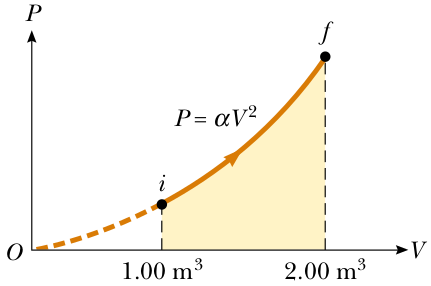
\includegraphics[scale=0.4]{17}
	%\end{figure}
	\begin{figure}[H]
		\centering
		\begin{tikzpicture}[scale=0.8]
		\begin{scope}
		\coordinate [label=above:$i$] (i) at (1,0.5);
		\coordinate [label=left:$f$] (f) at (3,4.4);
		\draw (0,0)-- (4,0);
		\draw [dashed] (0,0.5)-- (1,0.5);
		\draw [dashed] (1,0)--(1,0.5);
		\draw [dashed] (3,0)--(3,4.5);
		\draw [dashed] (0,0)--(1,.5);
		\draw (0,0)-- (0,4.5);
		\draw(0,4.2) node [color=blue, right=.1cm]{$P\left(Pa\right)$};
		\draw(4,0) node [color=blue, right=.1cm]{$V\left(m^{3}\right)$};
		\draw [arrows = {-Latex[width=8pt, length=10pt]}] (2,2) -- (2.2,2.4);
		\draw [arrows = {-Latex[width=8pt, length=8pt]}] (1.7,1.5) -- (1.2,3);
		\path[domain=1:3,name path=C]plot(\x,{0.5*\x*\x});
		\path[domain=1:3,name path=X](1,0)node[below]{$ 1.00 $}--(3,0)node[below]{$ 2.00 $};
		\tikzfillbetween[of={C and X}]{pattern=north east lines,pattern color=cyan!20!black};
		%\tikzfillbetween[of={C and X}]{pattern=bricks,pattern color=magenta};
		\draw[domain=1:3,samples=50,magenta]plot(\x,{0.5*\x*\x});
		\node[right,text=blue] at (0,3.3){$ \displaystyle P=\alpha V^{2}$};
		\draw (1,0.5) node {$\bullet$};
		\draw (3,4.5) node {$\bullet$};
		\end{scope}
		\end{tikzpicture}
	\end{figure}
	\item មួយម៉ូលនៃឧស្ម័ន $\ce{O2}$ សន្មតថាវាជាឧស្ម័នបរិសុទ្ធ។
	\begin{enumerate}[k]
		\item ឧស្ម័នរីកនៅសីតុណ្ហភាពថេរ $T=310K$ ពីមាឌដើម $V_i=12L$ ទៅ $V_f=19L$។\\
		គណនាកម្មន្តក្នុងដំណើរការរីកមាឌរបស់ឧស្ម័ន។
		\item ឧស្ម័នរួមមាឌនៅសីតុណ្ហភាពថេរ $T=310K$ ពីមាឌ $V_{i}=19L$ ទៅ $V_{f}=12L$។\\
		គណនាកម្មន្តក្នុងដំណើរការរួមមាឌរបស់ឧស្ម័ន។\\
		គេឲ្យៈ $\ln\left(\frac{19}{12}\right)=0.46,~\ln\left(\frac{12}{19}\right)=-0.46$ និង $R=8.31J/mol\cdot K$
	\end{enumerate}
	\begin{formula}
		\begin{enumerate}[m]
			\item \emph{\kml កម្មន្តក្នុងករណីមាឌថេរ(លំនាំអុីសូករ)}
			\begin{align*}
			\text{ករណី}\quad :&\quad V=\text{ថេរ}\quad \text{គេបាន}\quad W=0
			\end{align*}
			\item \emph{\kml ថាមពលក្នុង និងបម្រែបម្រួលថាមពលក្នុងនៃឧស្ម័នៈ}
			\begin{enumerate}[k,2]
				\item ថាមពលក្នុងនៃឧស្ម័នៈ\\ គឺជាថាមពលសុីនេទិចសរុបនៃឧស្ម័ន។
				\begin{align*}
					\text{គេបាន}\quad:&\quad U=\frac{3}{2}nRT\\
					\text{ឬ}\quad:&\quad U=\frac{3}{2}Nk_{B}T
				\end{align*}
				\item បម្រែបម្រួលថាមពលក្នុងនៃឧស្ម័ន
				\begin{align*}
					\text{យើងបាន}\quad:&\quad \Delta U=U_{2}-U_{1}\\
					\text{នោះ}\quad:&\quad \Delta U =\frac{3}{2}nRT_{2}-\frac{3}{2}nRT_{1}\\
					\text{ដូចនេះ}\quad:&\quad \Delta U = \frac{3}{2}nR\Delta T
				\end{align*}
			\end{enumerate}
			\item \emph{\kml ច្បាប់ទី១ ទែម៉ូឌីណាមិចៈ}
			កម្តៅស្រូបដោយប្រព័ន្ធស្មើនឹងផលបូកកម្មន្តបង្កើតឡើងដោយប្រព័ន្ធ និងបម្រែបម្រួលថាមពលក្នុងនៃប្រព័ន្ធ។
				\begin{align*}
					\text{គេកំណត់សរសេរ}\quad :&\quad Q=W+\Delta U
				\end{align*}
			\item \emph{\kml កម្មន្តក្នុងករណីកម្តៅមិនប្តូរជាមួយមជ្ឍដ្ឋានក្រៅ(លំនាំអាដ្យាបាទិច)} ជាលំនាំមួយដែលគ្មានបណ្តូរ​ថាមពលកម្តៅ (មិនស្រូប និងមិនបញ្ចេញកម្តៅ) ជាមួយមជ្ឍដ្ឋានក្រៅ មានន័យថា $Q=0J$។
			\begin{align*}
				\text{តាមច្បាប់ទីមួយទែម៉ូឌីណាមិច}\quad :&\quad Q=W+\Delta U\quad\text{តែ}\quad Q=0\\
				\text{ដូចនេះ}\quad :&\quad W=-\Delta U
			\end{align*}
		\end{enumerate}
	\end{formula}
	\item នៅលក្ខខណ្ឌ {\en (STP)} ឧស្ម័ន $2.2mol$ ត្រូវបានបង្រួមមាឌពី $50L$ ទៅ​ $10L$ តាមលំនាំអុីសូទែម។
	\begin{enumerate}[k]
		\item គណនាកម្មន្តដែលធ្វើលើឧស្ម័ន។ គេឲ្យៈ $\ln\left(0.2\right)=-1.61$។
		\item គណនាកម្តៅដែលភាយចេញពីឧស្ម័ន។
	\end{enumerate}
	\item ម៉ាសុីនកម្តៅមួយបានបំពេញកម្មន្ត $250J$ ក្នុងរយៈពេលដែលថាមពលក្នុងរបស់ម៉ាសុីនថយចុះ $500J$។\\ តើក្នុងលំនាំនេះកម្តៅនៃប្រព័ន្ធមានតម្លៃប៉ុន្មាន?
	\item ចូរគណនាបម្រែបម្រួលថាមពលក្នុងរបស់ប្រព័ន្ធឧស្ម័នទែម៉ូឌីណាមិចពេលៈ
	\begin{enumerate}[k]
		\item ប្រព័ន្ធស្រូបបរិមាណកម្តៅ $2000J$ និងធ្វើកម្មន្ត $500J$។
		\item ប្រព័ន្ធស្រូបបរិមាណកម្តៅ $1200J$ និងទទួលកម្មន្ត $400J$។
		\item បរិមាណកម្តៅ $300J$ ត្រូវបានបំភាយចេញពីប្រព័ន្ធនៅពេលមាឌថេរ។
	\end{enumerate}
	\item គណនាបម្រែបម្រួលថាមពលក្នុងនៃប្រព័ន្ធក្នុងករណីនីមួយៗខាងក្រោមៈ
	\begin{enumerate}[k]
		\item ប្រព័ន្ធស្រូបកម្តៅ $5kcal$ និងបំពេញកម្មន្ត $7200J$។
		\item ប្រព័ន្ធស្រូបកម្តៅ $5kcal$ និងរងនូវកម្មន្ត $7200J$។
		\item ប្រព័ន្ធឧស្ម័នមានមាឌថេរ និងបំភាយកម្តៅអស់ $4kcal$។
	\end{enumerate}
	\item គេធ្វើកម្មន្ត $25kJ$ លើប្រព័ន្ធឧស្ម័ន។ ក្រោយមកកម្តៅ $1.5kcal$ បានភាយចេញពីប្រព័ន្ធ។ \\គណនាបម្រែបម្រួលថាមពលក្នុង។ $\left(1cal=4.186J\right)$ 
	\item ក្នុងប្រព័ន្ធទែម៉ូឌីណាមិចប្រព័ន្ធទទួលកម្មន្ត $200J$​និងទទួលកម្តៅ $500J$។ រកបម្រែបម្រួលថាមពលក្នុង។
	\item ចូរគណនាបម្រែបម្រួលថាមពលក្នុងរបស់ប្រព័ន្ធៈ
	\begin{enumerate}[k]
		\item ប្រព័ន្ធស្រូបបរិមាណកម្តៅ $500cal$ និងធ្វើកម្មន្ត $400J$។
		\item ប្រព័ន្ធស្រូបកម្តៅ $300cal$ និងទទួលកម្មន្ត $420J$។
		\item បរិមាណកម្តៅ $1200cal$ ត្រូវបានភាយចេញពីប្រព័ន្ធនៅពេលមាឌថេរ។ គេឲ្យ $1cal=4.19J$
	\end{enumerate}
	\item ចូរគណនាបម្រែបម្រួលថាមពលក្នុងរបស់ប្រព័ន្ធៈ
	\begin{enumerate}[k]
		\item ប្រព័ន្ធធ្វើកម្មន្ត $5.0J$ ខណៈវារីកអាដ្យាបាទិច។
		\item ខណៈប្រព័ន្ធរួមអាដ្យាបាទិច កម្មន្ត $80J$ ត្រូវបានធ្វើលើឧស្ម័ន។
	\end{enumerate}
	\item ឧស្ម័នមួយស្រូបយកកម្តៅ $6.4kJ$ និងបំពេញកម្មន្ត $1200J$ ក្នុងពេលលំនាំនេះវាបានបញ្ចេញកម្តៅទៅវិញ $2400J$។ គណនាបម្រែបម្រួលថាមពលក្នុងរបស់ឧស្ម័ន។
	\item ឧស្ម័នមួយមានមាឌ $10L$ ស្ថិតនៅក្រោមសម្ពាធ $2\times10^{5}Pa$ និងសីតុណ្ហភាព $20^\circ C$។ ក្នុងលំនាំអុីសូបារ ឧស្ម័ននោះបានស្រូបបរិមាណកម្តៅ $5000J$ ហើយថាមពលក្នុងរបស់វាកើន $2000J$។ គណនាៈ
	\begin{enumerate}[k,2]
		\item កម្មន្តដែលបានបំពេញដោយឧស្ម័ននោះ។
		\item មាឌនៃឧស្ម័ននៅភាពស្រេច។
		\item សីតុណ្ហភាពស្រេចនៃឧស្ម័ននោះ។
	\end{enumerate} 
	\item ក្នុងសុីឡាំងមួយមានឧស្ម័នបរិសុទ្ធម៉ូណូអាតូម $0.5mol$។ គេធ្វើឲ្យឧស្ម័ននេះរីកមាឌពី $5dm^3$ ទៅ​ $12.5dm^3$ តាមលំនាំអុីសូទែម។ គេដឹងថាកម្មន្តដែលបានធ្វើដោយឧស្ម័ន ក្នុងរយៈពេលនៃដំណើរការគឺ $1142J$។\\គេឲ្យៈ $R=8.31J/mol\cdot K$
	\begin{enumerate}[k]
		\item គណនាសីតុណ្ហភាពនៃឧស្ម័នក្នុងពេលដំណើរការ។
		\item គណនាថាមពលក្នុងនៃឧស្ម័ននៅត្រង់ទីតាំងស្រេច។
		\item គណនាថាមពលកម្តៅដែលស្រូបដោយប្រព័ន្ធក្នុងរយៈពេលនៃដំណើរការ។
	\end{enumerate}
	\item ចូរគណនាកម្មន្តតាមលំនាំនីមួយៗ​ និងកម្មន្តសរុបក្នុងដ្យាក្រាម $P-V$ ខាងក្រោមៈ
	\begin{figure}[H]
		\centering
		\begin{tikzpicture}[scale=1]
		\begin{scope}
		\draw [dashed,gray,very thin, xstep=1.0cm,ystep=1.0cm] grid (3.5,3.5);
		\fill [cyan!60] (2,0) -- (2,3) -- (3,3) -- (3,0) -- cycle;
		\pattern[pattern color=white,pattern=bricks] (2,0) -- (2,3) -- (3,3) -- (3,0) -- cycle;
		\fill [cyan!60] (1,0) -- (2,2) -- (2,0) -- cycle;
		\pattern[pattern color=white,pattern=bricks] (1,0) -- (2,2) -- (2,0) -- cycle;
		\draw (0,0)-- (4,0);
		\draw [dashed] (0,2)-- (2,2);
		\draw [dashed] (0,3)-- (3,3);
		\draw [ultra thick] (2,3)-- (3,3);
		\draw [ultra thick] (1,0)-- (2,2);
		\draw [ultra thick] (2,2)-- (2,3);
		\draw [dashed] (3,2)-- (3,3);
		\draw [dashed] (2,0)--(2,2);
		\draw [dashed] (3,2)-- (3,0);
		\draw (0,0)-- (0,4);
		\draw(0,3.9) node [color=blue, right=.1cm]{$P\left(kPa\right)$};
		\draw(0,2) node [color=blue, left=.1cm]{$140$};
		\draw(0,3) node [color=blue, left=.1cm]{$210$};
		\draw (1,-.3) node [color=blue]{$0.25$};
		\draw (2,-.3) node [color=blue]{$0.50$};
		\draw (3,-.3) node [color=blue]{$0.80$};
		\draw (4,0) node [color=blue, right=.1cm]{$V\left(m^{3}\right)$};
		\draw [arrows = {-Latex[width=10pt, length=10pt]}] (2.2,3) -- (2.7,3);
		\draw [arrows = {-Latex[width=10pt, length=10pt]}] (2,2.5) -- (2,2.7);
		\draw [arrows = {-Latex[width=10pt, length=10pt]}] (1.5,1) -- (1.7,1.4);
		\draw (1,0) node {$\bullet$};
		\draw (3,3) node {$\bullet$};
		\coordinate [label=above left:$A$] (A) at (1,0);
		\coordinate [label=above right:$B$] (B) at (3,3);
		\coordinate [label=left:$1$] (1) at (1.4,1.1);
		\coordinate [label=left:$2$] (2) at (1.9,2.5);
		\coordinate [label=above:$3$] (3) at (2.5,3);
		\end{scope}
		\end{tikzpicture}
	\end{figure}
	\item \begin{enumerate}[k]
		\item គណនាកម្មន្តដែលបានធ្វើដោយឧស្ម័នបរិសុទ្ធម៉ូណូអាតូម ដែលចេញពីចំណុច $A$ ទៅចំណុច $B$\\ដូចដែលបានបង្ហាញក្នុងរូប។
		\item បើសិនជានៅត្រង់ចំណុច $A$ សីតុណ្ហភាពនៃឧស្ម័នមានតម្លៃ $267K$។ \\តើវាមានសីតុណ្ហភាពប៉ុន្មានពេលនៅត្រង់ចំណុច $C$។
		\item តើបរិមាណកម្តៅប៉ុន្មានដែលត្រូវបានស្រូប ឬបញ្ចេញពីឧស្ម័នក្នុងកំឡុងពេលដំណើរការនេះ?
	\end{enumerate}
	\begin{figure}[H]
		\centering
		\begin{tikzpicture}[scale=1]
		\begin{scope}
		\draw [dashed,gray,very thin, xstep=1.0cm,ystep=1.0cm] grid (5.5,3.5);
		\fill [cyan!60] (1,0) -- (1,1) -- (2,1) -- (3,3) --(3,3) -- (4,2) -- (4,1)--(5,1) -- (5,0) -- cycle;
		\pattern[pattern color=white,pattern=bricks] (1,0) -- (1,1) -- (2,1) -- (3,3) --(3,3) -- (4,2) -- (4,1)--(5,1) -- (5,0) -- cycle;
		\draw (0,0)-- (6,0);
		\draw [ultra thick] (1,1)-- (2,1)--(3,3)--(4,2)--(4,1)--(5,1);
		\draw [dashed] (1,0)--(1,1);
		\draw [dashed] (5,1)-- (5,0);
		\draw (0,0)-- (0,4);
		\draw(0,3.9) node [color=blue, right=.1cm]{$P\left(kPa\right)$};
		\draw(0,1) node [color=blue, left=.1cm]{$200$};
		\draw(0,2) node [color=blue, left=.1cm]{$400$};
		\draw(0,3) node [color=blue, left=.1cm]{$600$};
		\draw (1,-.3) node [color=blue]{$2.0$};
		\draw (2,-.3) node [color=blue]{$4.0$};
		\draw (3,-.3) node [color=blue]{$6.0$};
		\draw (4,-.3) node [color=blue]{$8.0$};
		\draw (5,-.3) node [color=blue]{$10$};
		\draw (6,0) node [color=blue, right=.1cm]{$V\left(m^{3}\right)$};
		\draw [arrows = {-Latex[width=10pt, length=10pt]}] (3.4,2.6) -- (3.6,2.4);
		\draw [arrows = {-Latex[width=10pt, length=10pt]}] (2.5,2) -- (2.6,2.2);
		\draw [arrows = {-Latex[width=10pt, length=10pt]}] (4.5,1) -- (4.7,1);
		\draw [arrows = {-Latex[width=10pt, length=10pt]}] (1.5,1) -- (1.7,1);
		\draw (1,1) node {$\bullet$};
		\draw (3,3) node {$\bullet$};
		\draw (5,1) node {$\bullet$};
		\coordinate [label=above left:$A$] (A) at (1,1);
		\coordinate [label=above right:$B$] (B) at (3,3);
		\coordinate [label=above right:$C$] (C) at (5,1);
		\end{scope}
		\end{tikzpicture}
	\end{figure}
	\item គណនាកម្មន្តសរុបក្នុងបម្លែងបិទ $ABCA$?
	\begin{figure}[H]
		\centering
		\begin{tikzpicture}
			\begin{scope}
				\draw (0,0)-- (0,4);
				\draw (0,0)-- (4,0);
				\draw [ultra thick] (1,1) -- (1,3) -- (3,1) --cycle;
				\coordinate [label=above:$A$] (A) at (1,3);
				\coordinate [label=right:$B$] (B) at (3,1);
				\coordinate [label=above left:$C$] (C) at (1,1);
				\draw [dashed] (1,0) --(1,1);
				\draw [dashed] (0,1) --(1,1);
				\draw [dashed] (0,3) --(1,3);
				\draw [dashed] (3,0) --(3,1);
				\fill [cyan!60] (1,1) -- (1,3) -- (3,1)--cycle;
				\pattern [pattern color=white, pattern=bricks] (1,1) -- (1,3) -- (3,1)--cycle;
				\coordinate [label=right:$V$] ($V$) at (4,0);
				\coordinate [label=below:$2.0m^{3}$] ($V_{1}$) at (1,0);
				\coordinate [label=below:$5.0m^{3}$] ($V_{2}$) at (3,0);
				\coordinate [label=left:$P$] ($P$) at (0,4);
				\coordinate [label=left:$1.0 atm$] ($P_{1}$) at (0,1);
				\coordinate [label=left:$2.0 atm$] ($P_{2}$) at (0,3);
				\draw [arrows = {-Latex[width=10pt, length=10pt]}] (1,2) -- (1,2.2);
				\draw [arrows = {-Latex[width=10pt, length=10pt]}] (2,1) -- (1.8, 1);
				\draw [arrows = {-Latex[width=10pt,length=10pt]}] (2,2)--(2.2,1.8);
			\end{scope}
		\end{tikzpicture}
	\end{figure}
	\item ឧស្ម័នបរិសុទ្ធមួយធ្វើបម្លែងបិទពីភាព $A$ រួចទៅភាព $B$ រួចទៅភាព $C$ ហើយទៅភាព $D$ ទៀត។ ក្រោយត្រឡប់មកភាពដើមវិញដូចបង្ហាញក្នុងរូប។ ចូរគណនាៈ
	\begin{multicols}{2}
		\begin{enumerate}[k]
			\item គណនាកម្មន្ត $AB,~BC,~CD$ និង $DA$។
			\item កម្មន្តសរុបក្នុងបម្លែងបិទ។
			\item កម្តៅដែលទទួលបានក្នុងបម្លែងបិទ។
		\end{enumerate}
		\begin{figure}[H]
			\centering
			\begin{tikzpicture}[scale=1]
			\begin{scope}
			\draw (0,0)-- (0,4);
			\draw (0,0)-- (4,0);
			\draw [ultra thick] (1,1) -- (1,3) -- (3,3) --(3,1) --cycle;
			\coordinate [label=above:$A$] (A) at (1,3);
			\coordinate [label=above:$B$] (B) at (3,3);
			\coordinate [label=right:$C$] (C) at (3,1);
			\coordinate [label=below left:$D$] (D) at (1,1);
			\draw [dashed] (1,0) --(1,1);
			\draw [dashed] (0,1) --(1,1);
			\draw [dashed] (0,3) --(1,3);
			\draw [dashed] (3,0) --(3,1);
			\fill [cyan!60] (1,1) -- (1,3) -- (3,3) -- (3,1)--cycle;
			\pattern [pattern color=white, pattern=bricks] (1,1) -- (1,3) -- (3,3) -- (3,1)--cycle;
			\coordinate [label=right:$V\left(L\right)$] ($V$) at (4,0);
			\coordinate [label=below:$2.0$] ($V_{1}$) at (1,0);
			\coordinate [label=below:$4.0$] ($V_{2}$) at (3,0);
			\coordinate [label=left:$P\left(atm\right)$] ($P$) at (0,4);
			\coordinate [label=left:$1.0$] ($P_{1}$) at (0,1);
			\coordinate [label=left:$2.0$] ($P_{2}$) at (0,3);
			\draw [arrows = {-Latex[width=10pt, length=10pt]}] (1,2) -- (1,2.2);
			\draw [arrows = {-Latex[width=10pt, length=10pt]}] (2,1) -- (1.8, 1);
			\draw [arrows = {-Latex[width=10pt,length=10pt]}] (3,2)--(3,1.8);
			\draw [arrows = {-Latex[width=10pt,length=10pt]}] (2.3,3)--(2.5,3);
			\end{scope}
			\end{tikzpicture}
		\end{figure}
	\end{multicols}
	\item ឧស្ម័នមួយស្ថិតក្នុងសុីឡាំងបិទជិតដោយពីស្តុងដែលអាចផ្លាស់ទីដោយគ្មានកកិត និងស្ថិតក្រោមសម្ពាធបរិយាកាស។ នៅពេលដែលកម្តៅ $254kcal$​ត្រូបានផ្តល់ឲ្យឧស្ម័ន មាឌរបស់វាកើនឡើងពី $12.0m^{3}$ ទៅដល់​ $16.2m^{3}$។
	\begin{enumerate}[k]
		\item គណនាកម្មន្តដែលបំពេញដោយឧស្ម័ន។
		\item គណនាបម្រែបម្រួលថាមពលក្នុងនៃឧស្ម័ន។
	\end{enumerate}
	\item គេបញ្ចុះសីតុណ្ហភាពអេល្យូមដែលមានមាឌដើម $1.0m^{3}$ នៅសីតុណ្ហភាព $0^\circ C$ និងសម្ពាធថេរ $1.0atm$ រហូតដល់ត្រឹមមាឌ $0.75m^{3}$។ គណនាបរិមាណកម្តៅ។
	\item ដូចបង្ហាញក្នុងរូប ឧស្ម័នរីកមាឌពី $V_{0}$ ទៅ $4V_{0}$ ហើយសម្ពាធថយចុុះពី $P_{0}$ ទៅ $P_{0}=\frac{P_{0}}{4}$។ គេដឹងថា $V_{0}=1.0m^{3}$  ហើយ $P_{0}=40Pa$។ ចូរគណនាកម្មន្តដែលបំពេញដោយឧស្ម័នប្រសិនបើសម្ពាធ និងមាឌឧស្ម័នប្រែប្រួល។
	\begin{multicols}{2}
		\begin{enumerate}[k]
			\item តាមគន្លង $\left(A\right)$។
			\item តាមគន្លង $\left(B\right)$។
			\item តាមគន្លង $\left(C\right)$។
		\end{enumerate}
		\begin{figure}[H]
			\centering
			\begin{tikzpicture}[scale=1]
			\begin{scope}
			\draw [dashed,gray,very thin, xstep=1.0cm,ystep=1.0cm] grid (4.5,4.5);
			\draw (0,0)-- (0,4.5);
			\draw (0,0)-- (4.5,0);
			\draw [color=magenta, ultra thick] (4,1) -- (1,1) -- (1,4);
			\draw [color=green!30!black, ultra thick] (1,4) -- (4,4) -- (4,1);
			\draw [color=yellow!10!orange, ultra thick] (1,4) -- (4,1);
			\coordinate [label=below:$0$] (0) at (0,0);
			\coordinate [label=above:$A$] (A) at (2.5,4);
			\coordinate [label=above right:$B$] (B) at (2,3);
			\coordinate [label=right:$C$] (C) at (1,2.5);
			\coordinate [label=below:$V_{0}$] ($V_{0}$) at (1,0);
			\coordinate [label=below:$4V_{0}$] ($V_{4}$) at (4,0);
			\coordinate [label=left:$P_{0}$] ($P_{0}$) at (0,4);
			\draw [color=magenta, arrows = {-Latex[width=10pt, length=10pt]}] (1,2.5) -- (1,2.3);
			\draw [color=magenta, arrows = {-Latex[width=10pt, length=10pt]}] (2.5,1) -- (2.7, 1);
			\draw [color=yellow!10!orange, arrows = {-Latex[width=10pt,length=10pt]}] (2.5,2.5)--(2.6,2.4);
			\draw [color=green!30!black, arrows = {-Latex[width=10pt,length=10pt]}] (2.5,4)--(2.7,4);
			\draw [color=green!30!black, arrows = {-Latex[width=10pt, length=10pt]}] (4,2.5) -- (4,2.3);
			\draw [color=black] (1,4) node {$\bullet$};
			\draw [color=black] (4,1) node {$\bullet$};
			\end{scope}
			\end{tikzpicture}
		\end{figure}
	\end{multicols}
	\item \begin{multicols}{2}
		ឧស្ម័នមួយនៅក្នុងធុងបិទជិត ដំណើរការក្នុងវដ្តដូចបង្ហាញក្នុងលើក្រាប $P-V$។ មាត្រដ្ឋានដេកកំណត់ឲ្យតម្លៃ $V_{s}=4.0m^{3}$ និងមាត្រដ្ឋានឈរកំណត់ឲ្យសម្ពាធគិតជា $\left(N/m^{2}\right)$។\\ គណនាថាមពលកម្តៅក្នុងមួយដំណើរការពេញនៃវដ្ត។
			\begin{figure}[H]
			\centering
			\begin{tikzpicture}[scale=1]
			\begin{scope}
			\draw [dashed,gray,very thin, xstep=1.0cm,ystep=1.0cm] grid (4.5,4.5);
			\draw (0,0)-- (0,4.5);
			\draw (0,0)-- (4.5,0);
			\draw [color=magenta, ultra thick] (1,1) -- (4,3) -- (1,3)--cycle;
			\coordinate [label=below:$A$] (A) at (1,1);
			\coordinate [label=above:$B$] (B) at (4,3);
			\coordinate [label=above:$C$] (C) at (1,3);
			\coordinate [label=below:$0$] (0) at (0,0);
			\coordinate [label=below:$V_{s}$] ($V_{s}$) at (4,0);
			\coordinate [label=left:$40$] ($40$) at (0,4);
			\coordinate [label=left:$30$] ($30$) at (0,3);
			\coordinate [label=left:$20$] ($20$) at (0,2);
			\coordinate [label=left:$10$] ($10$) at (0,1);
			\draw [color=magenta, arrows = {-Latex[width=10pt, length=10pt]}] (2.5,2) -- (2.7,2.1);
			\draw [color=magenta, arrows = {-Latex[width=10pt,length=10pt]}] (2.5,3)--(2.3,3);
			\draw [color=magenta, arrows = {-Latex[width=10pt, length=10pt]}] (1,2) -- (1,1.8);
			\draw [color=black] (1,1) node {$\bullet$};
			\draw [color=black] (4,3) node {$\bullet$};
			\draw [color=black] (1,3) node {$\bullet$};
			\end{scope}
			\end{tikzpicture}
		\end{figure}
	\end{multicols}
	\item គេធ្វើកម្មន្តលើប្រព័ន្ធមួយ $200J$ ហើយកម្តៅ $70.0cal$ ត្រូវបានភាយចេញពីប្រព័ន្ធ។ \\ដោយប្រើច្បាប់ទីមួយទែម៉ូឌីណាមិចៈ
	\begin{enumerate}[k]
		\item ទាញរកកម្មន្ត $\left(W\right)$ ដោយបញ្ជាក់សញ្ញា និងពន្យល់ហេតុផល។
		\item កំណត់សញ្ញា $\left(Q\right)$ ព្រមទាំងពន្យល់ហេតុផល។
		\item គណនាបម្រែបម្រួលថាមពលក្នុង $\left(\Delta U\right)$។ តើថាមពលក្នុងថយចុះ ឬកើនឡើង?
	\end{enumerate}
	\item \begin{enumerate}[k]
		\item ពិសីរត់ហាត់ប្រាណតាមបណ្តោយឆ្នេរសមុទ្រដោយបំពេញកម្មន្ត $4.3\times10^{5}J$ និងបញ្ចេញកម្តៅ $3.8\times10^{5}J$។ គណនាបម្រែបម្រួលថាមពលក្នុង ក្នុងខ្លួនពិសី។
		\item បើនាងប្តូរពីរត់មកដើរវិញ នោះនាងបញ្ចេញកម្តៅអស់ $1.2\times10^{5}J$ និងថាមពលក្នុងថយចុះអស់ $2.6\times10^{5}J$។ តើកំឡុងពេលដើរ ពិសីបំពេញកម្មន្តបានប៉ុន្មាន?
	\end{enumerate}
	\item ក្នុងសុីឡាំងមួយមានឧស្ម័នបរិសុទ្ធម៉ូណូអាតូម $0.5mol$ នៅសីតុណ្ហភាព $310K$។\\ ដោយរក្សាសីតុណ្ហភាពថេរ ឧស្ម័នរីកមាឌពី $310dm^{3}$ រហូតដល់ $450dm^{3}$។ គេឲ្យៈ $\ln\left(1.45\right)=0.37$
	\begin{enumerate}[k,2]
		\item គណនាកម្មន្តដែលប្រព័ន្ធបញ្ចេញ។
		\item គណនាបម្រែបម្រួលថាមពលក្នុងរបស់ឧស្ម័ន។
		\item គណនាកម្តៅស្រូបដោយឧស្ម័នក្នុងពេលបម្រែបម្រួលមាឌ។
	\end{enumerate}
	\item គណនាបម្រែបម្រួលថាមពលក្នុងនៃប្រព័ន្ធក្នុងករណីនីមួយៗ ដូចខាងក្រោមៈ
	\begin{enumerate}[k]
		\item ប្រព័ន្ធស្រូបកម្តៅ $500cal$ និងបញ្ចេញកម្មន្ត $400J$។
		\item ប្រព័ន្ធស្រូមកម្តៅ $300cal$ និងរងកម្មន្ត $420J$។
		\item ប្រព័ន្ធឧស្ម័នមានមាឌថេរ និងបំភាយកម្តៅអស់ $1200cal$។
	\end{enumerate}
	\item ឧស្ម័នក្នុងធុងមួយមានសម្ពាធ $1.50atm$ និងមានមាឌ $4.00m^{3}$។ គណនាកម្មន្តៈ
	\begin{enumerate}[k]
		\item បើឧស្ម័នរីកមាឌពីរដងនៃមាឌដើម និងរក្សាសម្ពាធថេរ។
		\item បើគេបណ្ណែនឧស្ម័នមក $\frac{1}{4}$ នៃមាឌដើម និងសម្ពាធថេរ។
	\end{enumerate}
	\item ឧស្ម័នបរិសុទ្ធមួយត្រូវបានបង្រួមដោយសម្ពាធថេរ $0.8atm$ ពីមាឌ $9.0L$ ទៅ $2.0L$។\\
	ក្នុងលំនាំនេះឧស្ម័នបញ្ចេញកម្តៅ $400J$។ គណនាៈ
	\begin{enumerate}[k]
		\item កម្មន្តនៃដំណើរការរបស់ឧស្ម័ន។
		\item បម្រែបម្រួលថាមពលក្នុងរបស់ឧស្ម័ន។
	\end{enumerate} 
	\item ឧស្ម័នបរិសុទ្ធមួយមានសីតុណ្ហភាពដើម $300K$ រងបម្លែងទែម៉ូឌីណាមិចតាមលំនាំអុីសូបារពីមាឌ $1.00m^{3}$ ទៅ $3.00m^{3}$ នៅសម្ពាធ $2.50kPa$។ កម្តៅ $12.5kJ$ ត្រូវបានស្រូបដោយឧស្ម័ន។
	\begin{enumerate}[k]
		\item គណនាបម្រែប្រួលថាមពលក្នុងរបស់ឧស្ម័ន។
		\item សីតុណ្ហភាពចុងក្រោយរបស់ឧស្ម័ន។
	\end{enumerate} 
	\item ឧស្ម័នបរិសុទ្ធមួយត្រូវបានឆ្លងកាត់នៃវដ្តដំណើរការដូចរូប។
	\begin{multicols}{2}
		\begin{enumerate}[k]
			\item គណនាថាមពលកម្តៅសរុបក្នុងបម្លែងបិទ។
			\item បើឧស្ម័នប្រព្រឹត្តក្នុងវដ្តបញ្ច្រាស $ACBA$ វិញ។\\​
			គណនាថាមពលកម្តៅសរុបក្នុងវដ្តបញ្ច្រាស។
		\end{enumerate}
		\begin{figure}[H]
			\centering
			\begin{tikzpicture}[scale=1]
			\begin{scope}
			\draw [dashed,gray,very thin, xstep=1.0cm,ystep=1.0cm] grid (3.1,4.1);
			\draw (0,0)-- (0,4.5);
			\draw (0,0)-- (3.5,0);
			\fill [cyan!60] (1,1) -- (3,4) -- (3,1) --cycle;
			\pattern [pattern color=white, pattern=bricks] (1,1) -- (3,4) -- (3,1) --cycle;
			\draw [ultra thick] (1,1) -- (3,4) -- (3,1)--cycle;
			\coordinate [label=above left:$A$] (A) at (1,1);
			\coordinate [label=above:$B$] (B) at (3,4);
			\coordinate [label=right:$C$] (C) at (3,1);
			\coordinate [label=below:$0$] (0) at (0,0);
			\coordinate [label=right:$V\left(m^{3}\right)$] ($V$) at (3.5,0);
			\coordinate [label=below:$6.0$] ($6.0$) at (1,0);
			\coordinate [label=below:$8.0$] ($8.0$) at (2,0);
			\coordinate [label=below:$10$] ($10$) at (3,0);
			\coordinate [label=above:$P\left(kPa\right)$] ($P$) at (0,4.5);
			\coordinate [label=left:$8.0$] ($8.0$) at (0,4);
			\coordinate [label=left:$6.0$] ($6.0$) at (0,3);
			\coordinate [label=left:$4.0$] ($4.0$) at (0,2);
			\coordinate [label=left:$2.0$] ($2.0$) at (0,1);
			\draw [arrows = {-Latex[width=10pt, length=10pt]}] (3,2.5) -- (3,2.3);
			\draw [arrows = {-Latex[width=10pt,length=10pt]}] (2,1)--(1.8,1);
			\draw [arrows = {-Latex[width=10pt, length=10pt]}] (2,2.5) -- (2.1,2.6);
			\draw [color=black] (1,1) node {$\bullet$};
			\draw [color=black] (3,1) node {$\bullet$};
			\draw [color=black] (3,4) node {$\bullet$};
			\draw [dashed] (0,1)--(1,1);
			\draw [dashed] (0,4)--(3,4);
			\draw [dashed] (1,0)--(1,1);
			\draw [dashed] (3,0)--(3,1);
			\end{scope}
			\end{tikzpicture}
		\end{figure}
	\end{multicols}
	\item ក្នុងរូបបង្ហាញពីវដ្តនៃឧស្ម័ន។ បម្រែបម្រួលថាមពលក្នុងនៃឧស្ម័នក្នុងលំនាំពី $a\rightarrow c$ តាមគន្លង $abc$ គឺ $-200J$។ ថាមពល $180J$ ត្រូវបានផ្តល់ជាកម្តៅក្នុងលំនាំពី $c\rightarrow d$។\\ ម្យ៉ាងទៀតថាមពល $80J$ ត្រូវបានផ្តល់ជាកម្តៅក្នុងលំនាំពី $d\rightarrow a$។\\ ចូរគណនាកម្មន្តដែលបំពេញដោយឧស្ម័នក្នុងលំនាំពី $c\rightarrow d$។
		\begin{figure}[H]
		\centering
		\begin{tikzpicture}[scale=1.5]
		\begin{scope}
		\draw (0,0)-- (0,3.5);
		\draw (0,0)-- (3.5,0);
		\draw [ultra thick] (1,1) -- (3,1) -- (3,3) -- (1,2) --cycle;
		\coordinate [label=above:$a$] (a) at (3,3);
		\coordinate [label=above left:$b$] (b) at (1,2);
		\coordinate [label=left:$c$] (c) at (1,1);
		\coordinate [label=right:$d$] (c) at (3,1);
		\coordinate [label=right:$V$] ($V$) at (3.5,0);
		\coordinate [label=above:$P$] ($P$) at (0,3.5);
		\draw [arrows = {-Latex[width=10pt, length=10pt]}] (3,2) -- (3,2.2);
		\draw [arrows = {-Latex[width=10pt,length=10pt]}] (2,1)--(2.2,1);
		\draw [arrows = {-Latex[width=10pt,length=10pt]}] (1,1.5)--(1,1.3);
		\draw [arrows = {-Latex[width=10pt, length=10pt]}] (2,2.5) -- (1.6,2.3);
		\end{scope}
		\end{tikzpicture}
	\end{figure}
	\newpage
	\item ឧស្ម័នមួយត្រូវបានដាក់ឲ្យដំណើរការក្នុងវដ្ត $abca$ ដូចបង្ហាញក្នុងដ្យាក្រាម $\left(P-V\right)$។ កម្មន្តសរុបក្នុងបម្លែងបិទគឺ $1.2J$។ ក្នុងលំនាំ $ab$ បម្រែបម្រួលថាមពលក្នុងមានតម្លៃ $3.0J$​និងកម្មន្តបំពេញដោយឧស្ម័នគឺ $5.0J$។\\ ក្នុងលំនាំ $ca$ ថាមពល $2.5J$ ត្រូវបានផ្តល់ជាកម្តៅ។ ចូរគណនាថាមពលកម្តៅៈ
	\begin{multicols}{2}
		\begin{enumerate}
			\item ក្នុងលំនាំ $ab$។ 
			\item ក្នុងលំនាំ $bc$។
		\end{enumerate}
		\begin{figure}[H]
			\centering
			\begin{tikzpicture}[scale=1]
			\begin{scope}
			\draw (0,0)-- (0,3.5);
			\draw (0,0)-- (3.5,0);
			\draw [ultra thick] (1,1) -- (1,3) -- (3,3) -- cycle;
			\coordinate [label=above:$a$] (a) at (1,3);
			\coordinate [label=above:$b$] (b) at (3,3);
			\coordinate [label=below:$c$] (c) at (1,1);
			\coordinate [label=right:$V$] ($V$) at (3.5,0);
			\coordinate [label=above:$P$] ($P$) at (0,3.5);
			\draw [arrows = {-Latex[width=10pt,length=10pt]}] (2,3)--(2.2,3);
			\draw [arrows = {-Latex[width=10pt,length=10pt]}] (1,2)--(1,2.2);
			\draw [arrows = {-Latex[width=10pt, length=10pt]}] (2,2) -- (1.8,1.8);
			\end{scope}
			\end{tikzpicture}
		\end{figure}
	\end{multicols}
	\item កន្លះម៉ូលនែឧស្ម័នបរិសុទ្ធមួយត្រូវបានដំណើរការពីភាព $a$ ទៅភាព $c$ ដូចបង្ហាញក្នុងរូប។
	\begin{multicols}{2}
		\begin{enumerate}[k]
			\item គណនាសីតុណ្ហភាពស្រេចនៃឧស្ម័ន។
			\item គណនាកម្មន្តដែលបានធ្វើលើ ឬធ្វើដោយ ឧស្ម័នដែលចេញពីភាព $a$ ទៅ $c$។
			\item តើកម្តៅត្រូវបានភាយចេញពីប្រព័ន្ធ ឬស្រូបចូលប្រព័ន្ធក្នុងដំណើរការនេះ?\\
			តើបរិមាណកម្តៅមានតម្លៃប៉ុន្មាន? ចូរពន្យល់។
		\end{enumerate}
		\begin{figure}[H]
			\centering
			\begin{tikzpicture}[scale=1.2]
			\begin{scope}
			\draw [dashed,magenta, ultra thick, xstep=1.0cm] grid (4.1,.1);
			\draw [dashed,magenta,ultra thick, ystep=1.5cm] grid (.1,3.1);
			\draw [ultra thick, ystep=1.5cm] (0,0)-- (0,3.5);
			\draw [ultra thick, xstep=1.0cm] (0,0)-- (4.5,0);
			\draw [ultra thick] (2,3) -- (3,1.5);
			\draw [ultra thick, color=cyan] (3,1.5) -- (4,1.5);
			\coordinate [label=above:$a$] (a) at (2,3);
			\coordinate [label=below:$b$] (b) at (3,1.5);
			\coordinate [label=below:$c$] (c) at (4,1.5);
			\coordinate [label=right:$V\left(m^{3}\right)$] ($V$) at (4.5,0);
			\coordinate [label=above:$P\left(Pa\right)$] ($P$) at (0,3.5);
			\coordinate [label=left:$4.0\times10^5$] ($P$) at (0,3);
			\coordinate [label=left:$2.0\times10^5$] ($P$) at (0,1.5);
			\draw [arrows = {-Latex[width=10pt,length=10pt]}] (2.42,2.4)--(2.5,2.3);
			\draw [color=cyan, arrows = {-Latex[width=10pt, length=10pt]}] (3.5,1.5) -- (3.7,1.5);
			\coordinate [label=below:$0.001$] ($0.001$) at (1,0);
			\coordinate [label=below:$0.002$] ($0.002$) at (2,0);
			\coordinate [label=below:$0.003$] ($0.003$) at (3,0);
			\coordinate [label=below:$0.004$] ($0.004$) at (4,0);
			\draw [color=blue] (2,3) node {$\bullet$};
			\draw [color=blue] (3,1.5) node {$\bullet$};
			\draw [color=blue] (4,1.5) node {$\bullet$};
			\end{scope}
			\end{tikzpicture}
		\end{figure}
	\end{multicols}
	\item ពីរម៉ូលនៃឧស្ម័នបរិសុទ្ធមួយត្រូវបានកំដៅក្រោមសម្ពាធថេរ ពី $27^\circ C$ ទៅ $107^\circ C$។
	\begin{enumerate}[k]
		\item គូសដ្យាក្រាម $P-V$ សម្រាប់ដំណើរការនេះ។
		\item គណនាកម្មន្តដែលបានធ្វើដោយឧស្ម័ន។
	\end{enumerate}
	\item ប្រាំមួយម៉ូលនៃឧស្ម័នបរិសុទ្ធមួយស្ថិតនៅក្នុងស៊ីឡាំងបិទជិតដោយពីស្តុងដែលអាចចល័តបាន។ នៅភាពដើមសីតុណ្ហភាពរបស់ឧស្ម័នគឺ $27.0^\circ C$ និងស្ថិតក្រោមសម្ពាធថេរ។\\ គណនាសីតុណ្ហភាពស្រេចនៃឧស្ម័នបន្ទាប់ពីវាបានធ្វើកម្មន្ត $1.75\times10^{3}J$។ 
	\item ពីរម៉ូលនៃឧស្ម័នបរិសុទ្ធមួយត្រូវបានបង្រួមមាឌដោយដាក់ក្នុងសុីឡាំងមួយ ដោយរក្សាសីតុណ្ហភាពថេរ $85^\circ C$ រហូតដល់សម្ពាធដើមរបស់វាកើនឡើងបីដង។
	\begin{enumerate}[k]
		\item គូសដ្យាក្រាម $P-V$ សម្រាប់ដំណើរការនេះ។
		\item គណនាកម្មន្តដែលបានបំពេញដោយឧស្ម័ន។
	\end{enumerate}
	\item ចូរសរសេរទំនាក់ទំនង់កម្មន្តបំពេញដោយឧស្ម័នចេញពីភាព $\left(A\right)\rightarrow \left(C\right)$ (ក្នុងរូប) ក្នុងករណីៈ
	\begin{multicols}{2}
		\begin{enumerate}[k]
			\item ឧស្ម័នដំណើរការតាមគន្លង $ADC$។
			\item ឧស្ម័នដំណើរការតាមគន្លង $ABC$។
			\item ឧស្ម័នដំណើរការតាមគន្លងត្រង់ $AC$។
		\end{enumerate}
		\begin{figure}[H]
			\centering
			\begin{tikzpicture}[scale=0.9]
			\begin{scope}
			\draw (0,0)-- (0,3.5);
			\draw (0,0)-- (3.5,0);
			\draw [color=magenta, ultra thick] (1,1) -- (1,3) -- (3,3);
			\draw [color=green!40!black, ultra thick] (1,1) -- (3,1) -- (3,3);
			\draw [color=yellow!10!orange, ultra thick] (1,1) -- (3,3);
			\coordinate [label=below:$0$] (0) at (0,0);
			\coordinate [label=below left:$A$] (A) at (1,1);
			\coordinate [label=above left:$B$] (B) at (1,3);
			\coordinate [label=above right:$C$] (C) at (3,3);
			\coordinate [label=below right:$D$] (D) at (3,1);
			\coordinate [label=below:$V_{A}$] ($V_{A}$) at (1,0);
			\coordinate [label=below:$V_{C}$] ($V_{C}$) at (3,0);
			\coordinate [label=left:$P_{C}$] ($P_{C}$) at (0,3);
			\coordinate [label=left:$P_{A}$] ($P_{A}$) at (0,1);
			\coordinate [label=right:$V$] ($V$) at (3.5,0);
			\coordinate [label=left:$P$] ($P$) at (0,3.5);
			\draw [color=magenta, arrows = {-Latex[width=10pt, length=10pt]}] (1,2) -- (1,2.2);
			\draw [color=magenta, arrows = {-Latex[width=10pt,length=10pt]}] (2,3)--(2.2,3);
			\draw [color=green!40!black, arrows = {-Latex[width=10pt, length=10pt]}] (2,1) -- (2.2, 1);
			\draw [color=green!40!black, arrows = {-Latex[width=10pt, length=10pt]}] (3,2) -- (3,2.2);
			\draw [color=yellow!10!orange, arrows = {-Latex[width=10pt,length=10pt]}] (2,2)--(2.2,2.2);
			\draw [color=black] (1,1) node {$\bullet$};
			\draw [color=black] (1,3) node {$\bullet$};
			\draw [color=black] (3,3) node {$\bullet$};
			\draw [color=black] (3,1) node {$\bullet$};
			\draw [dashed] (0,1) -- (1,1);
			\draw [dashed] (1,0) -- (1,1);
			\draw [dashed] (0,3) -- (1,3);
			\draw [dashed] (3,0) -- (3,1);
			\end{scope}
			\end{tikzpicture}
		\end{figure}
	\end{multicols}
	\item តាមដ្យាក្រាមដូចរូប បង្ហាញពីដំណើរការនៃបម្លែងទែម៉ូឌីណាមិច ដែលគន្លង $ab$ មានកម្តៅ $150J$ ត្រូវបានស្រូបដោយប្រព័ន្ធ និងគន្លង $bd$ មានកម្តៅ $600J$​ត្រូវបានស្រូបដោយប្រព័ន្ធ។ គណនាៈ
	\begin{multicols}{2}
		\begin{enumerate}[k]
			\item បម្រែបម្រួលថាមពលក្នុង តាមគន្លង $ab$។
			\item បម្រែបម្រួលថាមពលក្នុង តាមគន្លង $abd$។
			\item បរិមាណកម្តៅសរុប តាមគន្លង $acd$។
		\end{enumerate}
		\begin{figure}[H]
			\centering
			\begin{tikzpicture}[xscale=1.5]
			\begin{scope}
			\draw (0,0)-- (0,3.5);
			\draw (0,0)-- (3.7,0);
			\draw [color=magenta, ultra thick] (1,1) -- (1,3) -- (3,3);
			\draw [color=green!40!black, ultra thick] (1,1) -- (3,1) -- (3,3);
			\coordinate [label=below:$0$] (0) at (0,0);
			\coordinate [label=below left:$a$] (a) at (1,1);
			\coordinate [label=above left:$b$] (b) at (1,3);
			\coordinate [label=below right:$c$] (c) at (3,1);
			\coordinate [label=above right:$d$] (d) at (3,3);
			\coordinate [label=below:$2.0\times10^{-3}m^{3}$] ($V_{1}$) at (1,0);
			\coordinate [label=below:$5.0\times10^{-3}m^{3}$] ($V_{2}$) at (3,0);
			\coordinate [label=left:$8.0\times10^{4} Pa$] ($P_{2}$) at (0,3);
			\coordinate [label=left:$3.0\times10^{4} Pa$] ($P_{1}$) at (0,1);
			\coordinate [label=right:$V$] ($V$) at (3.7,0);
			\coordinate [label=left:$P$] ($P$) at (0,3.5);
			\draw [color=magenta, arrows = {-Latex[width=10pt, length=10pt]}] (1,2) -- (1,2.2);
			\draw [color=magenta, arrows = {-Latex[width=10pt,length=10pt]}] (2,3)--(2.2,3);
			\draw [color=green!40!black, arrows = {-Latex[width=10pt, length=10pt]}] (2,1) -- (2.2, 1);
			\draw [color=green!40!black, arrows = {-Latex[width=10pt, length=10pt]}] (3,2) -- (3,2.2);
			\draw [color=black] (1,1) node {$\bullet$};
			\draw [color=black] (1,3) node {$\bullet$};
			\draw [color=black] (3,3) node {$\bullet$};
			\draw [color=black] (3,1) node {$\bullet$};
			\draw [dashed] (0,1) -- (1,1);
			\draw [dashed] (1,0) -- (1,1);
			\draw [dashed] (0,3) -- (1,3);
			\draw [dashed] (3,0) -- (3,1);
			\end{scope}
			\end{tikzpicture}
		\end{figure}
	\end{multicols}
	\item ប្រព័ន្ធទែម៉ូឌីណាមិចមួយត្រូវបានដំណើរការពីភាព $a$ ទៅភាព $c$ ដូចបង្ហាញក្នុងរូប ដែលគន្លង $abc$ ប្រព័ន្ធធ្វើកម្មន្ត $450J$ និង $adc$ ប្រព័ន្ធធ្វើកម្មន្ត $120J$។ ថាមពលក្នុងតាមភាពនីមួយៗគឺ $U_{a}=150J,~U_{b}=240J,~U_{c}=680J$ និង $U_{d}=330J$។ គណនាបរិមាណកម្តៅស្រូបតាមគន្លងទាំងបួនគឺ $ab,~bc,~ad$ និង $dc$។
			\begin{figure}[H]
		\centering
		\begin{tikzpicture}[xscale=1.5]
		\begin{scope}
		\draw (0,0)-- (0,3.5);
		\draw (0,0)-- (3.7,0);
		\draw [color=magenta, ultra thick] (1,1) rectangle (3,3);
		\coordinate [label=below:$0$] (0) at (0,0);
		\coordinate [label=below left:$a$] (a) at (1,1);
		\coordinate [label=above left:$b$] (b) at (1,3);
		\coordinate [label=below right:$c$] (c) at (3,1);
		\coordinate [label=above right:$d$] (d) at (3,3);
		\coordinate [label=right:$V$] ($V$) at (3.7,0);
		\coordinate [label=left:$P$] ($P$) at (0,3.5);
		\draw [color=magenta, arrows = {-Latex[width=10pt, length=10pt]}] (1,2) -- (1,2.2);
		\draw [color=magenta, arrows = {-Latex[width=10pt,length=10pt]}] (2,3)--(2.2,3);
		\draw [color=magenta, arrows = {-Latex[width=10pt, length=10pt]}] (2,1) -- (2.2, 1);
		\draw [color=magenta, arrows = {-Latex[width=10pt, length=10pt]}] (3,2) -- (3,2.2);
		\draw [color=black] (1,1) node {$\bullet$};
		\draw [color=black] (1,3) node {$\bullet$};
		\draw [color=black] (3,3) node {$\bullet$};
		\draw [color=black] (3,1) node {$\bullet$};
		\end{scope}
		\end{tikzpicture}
	\end{figure}
	\item ពីរម៉ូលនៃឧស្ម័នម៉ូណូអាតូមមួយដំណើរការក្នុងសិុច(វដ្ត) $abc$។ ដើម្បីបំពេញមួយសិុចនៃដំណើរការនេះ មាន $800J$ នៃថាមពលកម្តៅត្រូវបានភាយចេញពីឧស្ម័ន​ ដែលដំណើរការ $ab$ ស្ថិតក្រោមសម្ពាធថេរ និងដំណើរការ $bc$ ស្ថិតក្រោមមាឌថេរ។ ត្រង់ភាព $a$ និង $b$ មានសីតុណ្ហភាព $T_{a}=200K$ និង $T_{b}=300K$។ 
	\begin{enumerate}[k]
		\item គូសដ្យាក្រាម $PV$ តាងដំណើរការនៃសុិចនេះ។
		\item គណនាកម្មន្តរបស់ដំណើរការ $ca$។
	\end{enumerate}
	\item ក្នុងម៉ាសុីនម៉ាស៊ូតមួយ ខ្យល់ក្នុងសុីឡាំងប្រហែលស្តង់ដាសម្ពាធ និងសីតុណ្ហភាព ត្រូវបានបណ្ណែនដោយពីស្តុងទៅដល់ $1/6$ នៃមាឌដើម និងសម្ពាធប្រហែល $50atm$។ តើសីតុណ្ហភាពខ្យល់ដែលបានបណ្ណែនស្មើនឹងប៉ុន្មាន?
	\item គណនាបម្រែបម្រួលថាមពលក្នុង និងបម្រែបម្រួលសីតុណ្ហភាពសម្រាប់ពីរលំនាំនៃឧស្ម័នបរិសុទ្ធម៉ូណូអាតូម $1.0mol$៖
	\begin{enumerate}[k]
		\item $1500J$ នៃកម្តៅត្រូវបានផ្តល់ទៅឲ្យឧស្ម័ន និងឧស្ម័នមិនបានធ្វើកម្មន្ត ហើយក៏គ្មានកម្មន្តធ្វើមកលើប្រព័ន្ធដែរ។
		\item $1500J$ នៃកម្មន្តបានធ្វើមកលើឧស្ម័ន និងគ្មានកម្តៅត្រូវបានផ្តល់ឲ្យ ឬយកចេញពីឧស្ម័នទេ។
	\end{enumerate}
	\item $500J$ នៃកម្តៅត្រូវបានផ្តល់ទៅឲ្យ $2mol$ នៃឧស្ម័នបរិសុទ្ធម៉ូណូអាតូម មានសីតុណ្ហភាពដើម $500K$ ខណៈដែលឧស្ម័នធ្វើកម្មន្ត $7500J$។\\ តើសីតុណ្ហភាពស្រេចនៃឧស្ម័នស្មើនឹងប៉ុន្មាន?
	\item សីតុណ្ហភាព $5.0mol$ នៃឧស្ម័នអាកុងត្រូវបានថយពី $300K$ មក $250K$។
	\begin{enumerate}[k]
		\item គណនាបម្រែបម្រួលថាមពលក្នុងនៃឧស្ម័ន។
		\item គណនាបម្រែបម្រួលថាមពលសុីនេទិចមធ្យមនៃម៉ូលេគុល(អាតូម)អាកុង។
	\end{enumerate}
	\item ក្នុងស្ថានភាពនីមួយៗដូចខាងក្រោម ចូររកបម្រែបម្រួលថាមលក្នុងនៃប្រព័ន្ធៈ
	\begin{enumerate}[k]
		\item ប្រព័ន្ធនោះទទួលកម្តៅ $500cal$ ហើយនៅពេលជាមួយគ្នានោះវាធ្វើកម្មន្ត $400J$។
		\item ប្រព័ន្ធនោះទទួលកម្តៅ $300cal$ ហើយនៅពេលជាមួយគ្នានោះកម្មន្ត $420J$ បានធ្វើមកលើប្រព័ន្ធ។
		\item កម្តៅ $1200cal$ ត្រូវបានដកចេញពីឧស្ម័ន គេឃើញមាឌថេរ។ គេឲ្យៈ $1cal=4.2J$ 
	\end{enumerate}
	\item \begin{enumerate}[k]
		\item ក្នុងលំនាំមួយ $600J$ នៃកម្តៅត្រូវបានផ្តល់ទៅឲ្យប្រព័ន្ធខណៈដែលប្រព័ន្ធធ្វើកម្មន្តស្មើនឹង $9000J$។\\ គណនាបម្រែបម្រួលថាមពលក្នុងនៃប្រព័ន្ធ។
		\item ក្នុងលំនាំមួយ $675J$ នៃកម្តៅត្រូវបានស្រូបដោយប្រព័ន្ធមួយ ខណៈ $290J$  នៃកម្មន្តត្រូវបានធ្វើមកលើប្រព័ន្ធ។ គណនាបម្រែបម្រួលថាមពលក្នុងនៃប្រព័ន្ធ។
	\end{enumerate}
	\item ឧស្ម័នបរិសុទ្ធមួយមានសីតុណ្ហភាពថេរ $T=300K$ ក្នុងរយៈពេលបម្រែបម្រួលមាឌពី $V_{1}=0.31m^{3}$ ទៅ\\ $V_{2}=0.45m^{3}$ គេដឹងថា ឧស្ម័នមាន $n=0.5mol$។ គណនាកម្មន្តដែលបំពេញក្នុងពេលបម្រែបម្រួលមាឌនេះ។\\
	យក $\ln\left(0.31\right)=-0.17~;~\ln\left(0.45\right)=-0.79~;~\ln\left(1.45\right)=0.37$
	\item គណនាមាឌស្រេចនៃមួយម៉ូលនៃឧស្ម័នបរិសុទ្ធនៅភាពដើមវាមានសីតុណ្ហភាព $0^\circ C$ និងសម្ពាធ $1.0atm$។ ប្រសិនបើវាស្រូប $2000cal$ នៃថាមពលកម្តៅអំឡុងពេលរេវែសុីបរីកអុីសូទែម។\\
	យក $1cal=4.19J~;~e^{3.69}=40~;~1.0atm = 1.013\times10^{5}Pa$
	\item អំឡុងពេលបណ្ណែនមាឌ ក្រោមសីតុណ្ហភាពថេរ $250Pa$ មាឌនៃឧស្ម័នបរិសុទ្ធនោះថយចុះពី $0.80m^{3}$ មក $0.20m^{3}$។ សីតុណ្ហភាពដើមរបស់វាគឺ $360K$ និងឧស្ម័នបាត់បង់កម្តៅ $210J$។
	\begin{enumerate}[k]
		\item តើបម្រែបម្រួលថាមពលក្នុងនៃឧស្ម័នស្មើនឹងប៉ុន្មាន?
		\item គណនាសីតុណ្ហភាពស្រេចនៃឧស្ម័ន។
	\end{enumerate} 
	\item បីម៉ូលនៃឧស្ម័នបរិសុទ្ធម៉ូណូអាតូមមួយស្ថិតក្រោមសីតុណ្ហភាព $345K$ ដោយ $2438J$ នៃកម្តៅត្រូវបានផ្តល់ទៅឲ្យឧស្ម័ន និង $962J$ នៃកម្មន្តត្រូវបានធ្វើលើវា។ តើសីតុណ្ហភាពស្រេចរបស់ឧស្ម័នមានតម្លៃប៉ុន្មាន?
	\item ប្រព័ន្ធមួយឡើងកម្តៅ $2780J$ នៅក្រោមសម្ពាធថេរ $1.26\times10^{5}Pa$ និងថាមពលក្នុងរបស់វាកើនបាន $3990J$។\\ តើបម្រែបម្រួលមាឌនៃប្រព័ន្ធស្មើនឹងប៉ុន្មាន ហើយវាកើនឡើង ឬថយចុះ?
	\item ប្រព័ន្ធមួយឡើងកម្តៅ $1500J$ ខណៈដែលថាមពលក្នុងនៃប្រព័ន្ធកើនបាន $4500J$ និងមាឌថយចុះបាន $0.010m^{3}$។ សន្មតថា សម្ពាធនៃប្រព័ន្ធថេរ។ គណនាតម្លៃនៃសម្ពាធនោះ
	\item ឧស្ម័នគំរូម៉ូណូអាតូមមួយ ដូចបង្ហាញក្នុងដ្យាក្រាម $PV$ ខាងក្រោម គឺនៅត្រង់ $A$ មានសីតុណ្ហភាព $300K$។ គេឲ្យៈ $R=8.31J/mol\cdot K$
	\begin{multicols}{2}
		\begin{enumerate}[k]
			\item រកចំនួនម៉ូលរបស់ឧស្ម័នគំរូនេះ។
			\item រកសីតុណ្ហភាពត្រង់ $B,~C$ និងមាឌត្រង់ $C$។
			\item ឥឡូវចាត់ទុកថាយើងមានលំនាំពី\\ $A\rightarrow B,~B\rightarrow C$ និង $C\rightarrow A$។\\ ចូរដាក់ឈ្មោះឲ្យលំនាំនីមួយៗ។
			\item គណនាកម្មន្តសរុបនៃលំនាំ។\\ គេឲ្យៈ $\ln\left(0.005\right)=-5.29\\\ln\left(0.015\right)=-4.19~;~\ln\left(3\right)=1.09$
		\end{enumerate}
		\begin{figure}[H]
			\centering
			\begin{tikzpicture}[scale=1.3]
			\begin{scope}
			\draw [dashed,magenta, ultra thick, xstep=1.0cm] grid (3.1,.1);
			\draw [dashed,magenta,ultra thick, ystep=1.0cm] grid (.1,3.1);
			\draw [->, -Stealth, ultra thick, ystep=1.0cm] (0,0)-- (0,3.6);
			\draw [->,-Stealth, ultra thick, xstep=1.0cm] (0,0)-- (3.6,0);
			\draw [ultra thick] (1,1) -- (1,3) (1,1)--(3,1) (1,3) .. controls (1.7,1.7) .. (3,1);
			\coordinate [label=below:$A$] (A) at (1,1);
			\coordinate [label=above:$B$] (B) at (1,3);
			\coordinate [label=below:$C$] (C) at (3,1);
			\coordinate [label=right:$V\left(L\right)$] ($V$) at (3.5,0);
			\coordinate [label=above:$P\left(atm\right)$] ($P$) at (0,3.5);
			\coordinate [label=left:$3$] ($P_{3}$) at (0,3);
			\coordinate [label=left:$2$] ($P_{2}$) at (0,2);
			\coordinate [label=left:$1$] ($P_{1}$) at (0,1);
			\draw [arrows = {-Latex[width=10pt,length=10pt]}] (1,2.1)--(1,2.3);
			\draw [arrows = {-Latex[width=10pt, length=10pt]}] (2,1) -- (1.8,1);
			\draw [arrows = {-Latex[width=10pt, length=10pt]}] (1.6,2) -- (1.75,1.8);
			\coordinate [label=below:$5$] ($5$) at (1,0);
			\coordinate [label=below:$10$] ($10$) at (2,0);
			\coordinate [label=below:$15$] ($15$) at (3,0);
			\draw [color=blue] (1,1) node {$\bullet$};
			\draw [color=blue] (3,1) node {$\bullet$};
			\draw [color=blue] (1,3) node {$\bullet$};
			\end{scope}
			\end{tikzpicture}
		\end{figure}
	\end{multicols}\newpage
	\item ឧស្ម័នមួយស្ថិតក្រោមលំនាំពីរគឺ លំនាំទី១ មាឌថេរនៅ $0.200m^{3}$ និងសម្ពាធកើនពី $2.00\times10^{5}Pa$ ទៅ\\ $5.00\times10^{5}Pa$។ លំនាំទី២ គឺបណ្ណែនមាឌដល់ $0.120m^{3}$ នៅសម្ពាធថេរ $5.00\times10^{5}Pa$។
	\begin{enumerate}[k]
		\item គូសដ្យាក្រាម $PV$ បង្ហាញលំនាំទាំងពីរ។
		\item គណនាកម្មន្តសរុបដែលធ្វើដោយឧស្ម័នក្នុងលំនាំទាំងពីរ។
	\end{enumerate}
	\item សីតុណ្ហភាពនៃ $3mol$ របស់ឧស្ម័នបរិសុទ្ធម៉ូណូអាតូមមួយត្រូវបានកាត់បន្ថយសីតុណ្ហភាពពី $T_{i}=540K$ មក $350K$ តាមវីធីពីរផ្សេងគ្នា។ វិធីទី១ កម្តៅ $5500J$ ផ្តល់ទៅឲ្យឧស្ម័ន។ វិធីទី២ កម្តៅ $1500J$ ផ្តល់ទៅឲ្យឧស្ម័ន។ ក្នុងករណីនីមួយៗ ចូរគណនាៈ
	\begin{enumerate}[k]
		\item បម្រែបម្រួលថាមពលក្នុងនៃឧស្ម័ន។
		\item កម្មន្តសធ្វើដោយឧស្ម័ន។
	\end{enumerate}
	\item $2mol$ នៃឧស្ម័នម៉ូណូអាតូមអាកុង $\left(\ce{Ar}\right)$ រីកតាមលំនាំអុីសូទែមនៅសីតុណ្ហភាព $298K$ ពីមាឌដើម $V_{i}=0.025m^{3}$ ទៅមាឌស្រេច $V_{f}=0.050m^{3}$។ សន្មត់ថា អាកុងជាឧស្ម័នបរិសុទ្ធ ចូរគណនាៈ
	\begin{enumerate}[k]
		\item កម្មន្តធ្វើដោយឧស្ម័ន។
		\item បម្រែបម្រួលថាមពលក្នុងនៃឧស្ម័ន។
		\item កម្តៅដែលបានផ្តល់ឲ្យឧស្ម័ន។
	\end{enumerate} 
	\item ឧស្ម័នបរិសុទ្ធមួយស្ថិតក្រោមលំនាំដែលបណ្ណែនតាមអុីសូទែមពីមាឌដើម $4.00m^{3}$ ទៅមាឌស្រេច $3.00m^{3}$។ \\គេដឹងថា ឧស្ម័នមាន $3.50mol$ និងសីតុណ្ហភាពរបស់វាគឺ $10.0^\circ C$។
	\begin{enumerate}[k]
		\item គណនាកម្មន្តធ្វើដោយឧស្ម័ន។
		\item គណនាកម្តៅដែលផ្តល់រវាងឧស្ម័ន និងមជ្ឈដ្ឋានក្រៅ។
	\end{enumerate}
	\item ឧស្ម័នគំរូ {\en(Sample)} មួយរីកមាឌពី​ $V_{1}=1.0m^{3}$ និង $P_{1}=40Pa$ ទៅ $V_{2}=4.0m^{3}$ និង $P_{2}=10Pa$ តាមគន្លង $B$ ដ្យាក្រាម $P-V$ ដូចក្នុងរូប។ វាបានបណ្ណែនត្រឡប់មក $V_{1}$ វិញតាមគន្លង $A$ ឬគន្លង $C$ វិញ។
	\begin{multicols}{2}
		គណនាកម្មន្តសរុបដែលឧស្ម័នបានបំពេញៈ
		\begin{enumerate}[k]
			\item តាមគន្លង $BA$។
			\item តាមគន្លង $BC$
		\end{enumerate}
		\begin{figure}[H]
			\centering
			\begin{tikzpicture}[xscale=1.3, yscale=1.2]
			\begin{scope}
			\draw [->, -Stealth, ultra thick, ystep=1.0cm] (0,0)-- (0,3.6);
			\draw [->,-Stealth, ultra thick, xstep=1.0cm] (0,0)-- (3.6,0);
			\draw [color=magenta, ultra thick] (3,1) -- (1,1) -- (1,3);
			\draw [color=green!40!black, dashed, ultra thick] (1,3) -- (3,3) -- (3,1);
			\draw [color=yellow!10!orange, densely dotted, ultra thick] (1,3) -- (3,1);
			\coordinate [label=below:$0$] (0) at (0,0);
			\coordinate [label=above:$A$] (A) at (2,3);
			\coordinate [label=above right:$B$] (B) at (2,2);
			\coordinate [label=above:$C$] (C) at (2,1);
			\coordinate [label=right:$V$] ($V$) at (3.5,0);
			\coordinate [label=below:$V_{1}$] ($V_{1}$) at (1,0);
			\coordinate [label=below:$V_{2}$] ($V_{2}$) at (3,0);
			\coordinate [label=above:$P$] ($P$) at (0,3.5);
			\coordinate [label=left:$P_{1}$] ($P_{1}$) at (0,3);
			\coordinate [label=left:$P_{2}$] ($P_{2}$) at (0,1);
			\draw [dashed] (1,0) -- (1,1) -- (0,1);
			\draw [dashed] (0,3) -- (1,3);
			\draw [dashed] (3,0) -- (3,1);
			\draw [color=magenta, arrows = {-Latex[width=10pt, length=10pt]}] (1,1.8) -- (1,2);
			\draw [color=magenta, arrows = {-Latex[width=10pt, length=10pt]}] (2,1) -- (1.8, 1);
			\draw [color=yellow!10!orange, arrows = {-Latex[width=10pt,length=10pt]}] (1.8,2.2)--(2.2,1.8);
			\draw [color=green!40!black, arrows = {-Latex[width=10pt,length=10pt]}] (2,3)--(1.8,3);
			\draw [color=green!40!black, arrows = {-Latex[width=10pt, length=10pt]}] (3,2) -- (3,2.3);
			\draw [color=black] (1,3) node {$\bullet$};
			\draw [color=black] (3,1) node {$\bullet$};
			\end{scope}
			\end{tikzpicture}
		\end{figure}
	\end{multicols}
	\item សុីឡាំងនៃម៉ាសុីនមួយមានមុខកាត់ $A=1.0dm^{3}$។ នៅភាពដើមឧស្ម័នមួយមានមាឌ $V_{1}=0.2dm^{3}$។\\ ក្រោមសម្ពាធថេរ $P=7.5\times10^{5}Pa$ ឧស្ម័នធ្វើកម្មន្តទៅលើពីស្តុងឲ្យផ្លាស់ទីបានចម្ងាយ $\Delta x=0.4dm^{3}$។
	\begin{enumerate}[k]
		\item គណនាបម្រែបម្រួលមាឌក្នុងពេលដែលឧស្ម័នបំពេញកម្មន្ត។
		\item គណនាមាឌស្រេច។
		\item គណនាកម្មន្តដែលបំពេញដោយឧស្ម័ន។
	\end{enumerate} 
	\item ឧស្ម័នមួយរីកមាឌពី $300dm^{3}$ ទៅ $1000dm^{3}$ និងសម្ពាធកើនពី $20MPa$ ទៅដល់ $40MPa$។\\ គណនាកម្មន្តដែលបានបំពេញដោយឧស្ម័ន រួចគូសដ្យាក្រាម $P-V$ បញ្ជាក់បម្លែងនេះ។
	\item ឧស្ម័នគំរូមួយរីកមាឌពី $1m^{3}$ ទៅ $4m^{3}$ នៅពេលដែលសម្ពាធវាថយចុះពី $40Pa$ ទៅ $10Pa$។\\ គណនាកម្មន្តបំពេញដោយឧស្ម័នតាមគន្លងនីមួយៗដូចបង្ហាញក្នុងរូបៈ
	\begin{multicols}{2}
		\begin{enumerate}[k]
			\item គន្លង $A$
			\item គន្លង $B$
			\item គន្លង $C$
		\end{enumerate}
		\begin{figure}[H]
			\centering
			\begin{tikzpicture}[xscale=1.3, yscale=1,>=stealth]
			\begin{scope}
			\draw [->, -Stealth, ultra thick, ystep=1.0cm] (0,0)-- (0,3.6);
			\draw [->,-Stealth, ultra thick, xstep=1.0cm] (0,0)-- (3.6,0);
			\draw [color=magenta, ultra thick] (3,1) -- (1,1) -- (1,3);
			\draw [color=green!40!black,ultra thick] (1,3) -- (3,3) -- (3,1);
			\draw [color=yellow!10!orange, ultra thick] (1,3) -- (3,1);
			\coordinate [label=above:$A$] (A) at (2,3);
			\coordinate [label=above right:$B$] (B) at (2,2);
			\coordinate [label=above:$C$] (C) at (2,1);
			\coordinate [label=right:$V\left(m^{3}\right)$] ($V$) at (3.5,0);
			\coordinate [label=below:$1$] ($V_{1}$) at (1,0);
			\coordinate [label=below:$4$] ($V_{2}$) at (3,0);
			\coordinate [label=above:$P\left(Pa\right)$] ($P$) at (0,3.5);
			\coordinate [label=left:$40$] ($P_{1}$) at (0,3);
			\coordinate [label=left:$10$] ($P_{2}$) at (0,1);
			\draw [dashed] (1,0) -- (1,1) -- (0,1);
			\draw [dashed] (0,3) -- (1,3);
			\draw [dashed] (3,0) -- (3,1);
			\draw [color=magenta, arrows = {-Latex[width=10pt, length=10pt]}] (1,2) -- (1,1.8);
			\draw [color=magenta, arrows = {-Latex[width=10pt, length=10pt]}] (1.8,1) -- (2, 1);
			\draw [color=yellow!10!orange, arrows = {-Latex[width=10pt,length=10pt]}] (1.8,2.2)--(2.2,1.8);
			\draw [color=green!40!black, arrows = {-Latex[width=10pt,length=10pt]}] (1.8,3)--(2,3);
			\draw [color=green!40!black, arrows = {-Latex[width=10pt, length=10pt]}] (3,2.3) -- (3,2);
			\end{scope}
			\end{tikzpicture}
		\end{figure}
	\end{multicols}
	\item ឧស្ម័នបរិសុទ្ធ $2mol$ នៅសីតុណ្ហាភាព $0^\circ C$ ត្រូវបានធ្វើបម្លែងអុីសូទែមពីមាឌ $V_{A}=5L$ ទៅ $V_{B}=10L$ រួចកម្តៅដោយមាឌថេររហូតសម្ពាធថយចុះអស់ពាក់កណ្តាលបន្ទាប់មកបណ្ណែនតាមលំនាំអុីសូបាររហូតដល់មាឌ $5L$ វិញធ្វើឲ្យឧស្ម័នទៅដល់សីតុណ្ហភាពដើមវិញដោយមាឌថេរ។
	\begin{enumerate}[k]
		\item តាមដ្យាក្រាម $PV$ គូសខ្សែកោងតាងលំនាំបួននៃបម្រែបម្រួលភាពនៃឧស្ម័ននេះ។
		\item គណនាសម្ពាធត្រង់ភាព $A$ និង $B$។ គេឲ្យៈ $R=8.31J/mol\cdot K$
		\item គណនាកម្មន្តដែលឧស្ម័នបានបំពេញក្នុងបម្លែងបិទនេះ។
	\end{enumerate}
	\item ក្នុងសុីឡាំងមួយមានឧស្ម័នបរិសុទ្ធ $1.5mol$ នៅសីតុណ្ហភាព $37^\circ C$។ ដោយរក្សាសីតុណ្ហភាពដដែលឧស្ម័នបានរីកមាឌពី$450dm^{3}$ ទៅ $600dm^{3}$។
	\begin{enumerate}[k]
		\item គណនាកម្មនដែលបំពេញក្នុងរយៈពេលបម្រែបម្រួលមាឌ។ គេឲ្យៈ $R=8.31J/mol\cdot K$
		\item គណនាបម្រែបម្រួលថាមពលក្នុងនៃឧស្ម័ន។
		\item រកកម្តៅដែលស្រូបដោយប្រព័ន្ធក្នុងរយៈពេលបម្រែបម្រួលមាឌ។
	\end{enumerate}
	\item នៅក្នុងសុីឡាំងដែលមានពីស្តុងចល័តគេដាក់ឧស្ម័នបរិសុទ្ធមួយមាន $n mol$។ គេផ្តល់កម្តៅ $Q$ ឲ្យប្រព័ន្ធ ឧស្ម័នបានរីកមាឌពី $V_{1}$ ទៅ $V_{2}$ ដោយរក្សាសីតុណ្ហភាព $T$ ដដែលដូចរូប។\\ កម្មន្តដែលបានបំពេញដោយប្រព័ន្ធក្នុងពេលរីកមាឌនេះគឺ $500J$។
	\begin{enumerate}[k]
		\item តើបម្រែបម្រួលថាមពលក្នុងនៃប្រព័ន្ធមានតម្លៃប៉ុន្មាន?
		\item គណនាកម្តៅដែលផ្តល់ឲ្យប្រព័ន្ធ។
	\end{enumerate}
	\begin{figure}[H]
		\begin{subfigure}[t]{.5\textwidth}
			\centering
			\begin{tikzpicture}
			\begin{scope}[scale=1]
				\node [draw, cylinder, cylinder uses custom fill, cylinder body fill=gray!20, 
				cylinder end fill=gray!70, shape aspect=4, rotate=0, minimum width=3cm] (c1) at 
				(1.3,0){};
				\node [draw, cylinder, cylinder uses custom fill, cylinder body fill=gray!20, 
				cylinder end fill=gray!70, shape aspect=4, rotate=0, minimum width=3cm] (c2) at 
				(-1,0){};
				
				\node [draw, cylinder, cylinder body fill=gray!50, 
				cylinder end fill=gray!50, shape aspect=4, rotate=0, minimum height=6.7cm, minimum 
				width=3cm] (c) {};
				
				\draw[<->] (-3,2.8)--(1.3,2.8);
				\draw[dashed] (-3,2.8) -- (-3,0);
				\draw[dashed] (1.3,2.8) -- (1.3,1.5);
				\draw[<->] (-3,2)--(-1,2);
				\draw[dashed] (-1,2) -- (-1,1.5);
				%\draw[->] (4.5,0) node { \color{blue}\text{ពីស្តុង} } (4,0)--(2,0);
				%			\draw[|->] (-3,-2)--(5,-2);
				%			\draw (4.9,-2.3) node {$x$};
				%			\draw (1.3,-2.3) node {$x_{2}$};
				%			\draw[dashed] (1.3,-2) -- (1.3,-1.5);
				%			\draw (1.3,-2) node {$\bullet$};
				%			\draw (-1,-2.3) node {$x_{1}$};
				%			\draw[dashed] (-1,-2) -- (-1,-1.5);
				%			\draw (-1,-2) node {$\bullet$};
				
				\draw [line width=3pt, arrows = {-Latex[width=10pt,length=10pt]}] (-.5, 0) -- (.5, 0);
				
				\coordinate [label=$Q$] ($Q$) at (-2,-.3);
				\coordinate [label=$V_{1}$] ($V_{1}$) at (-2,2);
				\coordinate [label=$V_{2}$] ($V_{2}$) at (-.5,2);
			\end{scope}
			\end{tikzpicture}
			\subcaption{\koc សុីឡាំង}
		\end{subfigure}
		\begin{subfigure}[t]{.5\textwidth}
			\centering
			\begin{tikzpicture}[scale=1.2]
				\begin{scope}
				\draw (0.8,2.5) .. controls (1.5,1) .. (3.5,0.5);
				%\fill [red!80!orange]
				(1,2) .. controls (1,1.5) .. (3,0);
				%\pattern[pattern color=white,pattern=bricks]
				(1,2) .. controls (1,1.5) .. (3,0);
				\draw (0,0)-- (4,0);
				\draw [dashed] (1,2)-- (1,0);
				\draw [dashed] (3,0.6)-- (3,0);
				\draw (0,0)-- (0,3);
				\draw(0,2.9) node [color=blue, left=.1cm]{$P$};
				\draw(4,0) node [color=blue, right=.1cm]{$V$};
				\draw(1,-.3) node [color=blue]{$V_{1}$};
				\draw(3,-.3) node [color=blue]{$V_{2}$};
				\draw (1,2) node {$\bullet$};
				\draw (1,2) node [color=blue, right=.2cm]{$A$};
				\draw (3,.5) node [color=blue, above=0.2cm]{$B$};
				\draw (3,.6) node {$\bullet$};
				\end{scope}
			\end{tikzpicture}
			\subcaption{\koc ដ្យាក្រាម $P-V$}
		\end{subfigure}
	\end{figure}
	\item គេបញ្ចុះសីតុណ្ហភាពអេល្យូមដែលមានមាឌដើម $1.0m^{3}$ នៅសីតុណ្ហភាព $0^\circ C$ និងសម្ពាធថេរ $1.0atm$ រហូតដល់ត្រឹម $0.75m^{3}$។ គណនាបរិមាណកម្តៅភាយចេញ។
	\item ទឹកដែលមានម៉ាស $1kg$ នៅសីតុណ្ហភាព $100^\circ C$ មានមាឌប្រហែល $1\times10^{-3}m^{3}$។ ក្នុងដំណើរការមួយគេដឹងថាចំហាយទឹកនៅ ពេលកម្តៅនៅសីតុណ្ហភាពនេះ និងសម្ពាធបរិយាកាសគំរូមានមាឌ $1.671m^{3}$។
	\begin{enumerate}
		\item គណនាកម្មន្តដែលបានធ្វើដើម្បីបញ្ចូនកម្តៅទៅបរិយាកាសវិញ។
		\item គណនាកំណើនថាមពលក្នុងពេលអង្គធាតុរាវផ្លាស់ប្តូរភាពទៅជាចំហាយទឹក\\ បើចំហាយទឹកមានកម្តៅឡាតង់ $L=540kcal/kg$។
	\end{enumerate}
	\item មួយក្រាមនៃទឹក $\left(1cm^{3}\right)$ ក្លាយជាចំហាយទឹក $1671cm^{3}$ ពេលវាពុះក្រោមសីតុណ្ហភាពថេរ $1atm\left(1.013\times10^{5}Pa\right)$។ កម្តៅឡាតង់នៃចំហាយទឹកគឺ $L_{V}=2.256\times10^{6}J/kg$។ ចូរគណនាៈ
	\begin{enumerate}[k]
		\item កម្មន្តដែលបានធ្វើដោយចំហាយទឹក។
		\item កំណើនថាមពលក្នុងរបស់វា។
	\end{enumerate}
	\item គេមានឧស្ម័នអេល្យូម $1.00kmol$ ឆ្លងកាត់វដ្តនៃដំណើរការម៉ាសុីនមួយដែលបង្ហាញតាមដ្យាក្រាមដូចរូប។ $BC$ គឺជាលំនាំអុីសូទែម និង $P_{A}=1.00atm,~V_{A}=22.4m^{3},~P_{B}=2.00atm$។
	\begin{multicols}{2}
		គេចាត់ទុកឧស្ម័ននេះជាឧស្ម័នបរិសុទ្ធ។
		\begin{enumerate}[k]
			\item គណនាសីតុណ្ហភាព $T_{A},~T_{B}$ និងមាឌ $V_{C}$។
			\item គណនាកម្មន្តដែលផ្តល់ឲ្យមជ្ឈដ្ឋានក្រៅ។ 
		\end{enumerate}
		\begin{figure}[H]
			\centering
			\begin{tikzpicture}[scale=1.3]
			\begin{scope}
			\draw [->, -Stealth, ultra thick, ystep=1.0cm] (0,0)-- (0,3.6);
			\draw [->,-Stealth, ultra thick, xstep=1.0cm] (0,0)-- (3.6,0);
			\draw [ultra thick] (1,1) -- (1,3) (1,1)--(3,1) (1,3) .. controls (1.7,1.7) .. (3,1);
			\coordinate [label=below:$A$] (A) at (1,1);
			\coordinate [label=above:$B$] (B) at (1,3);
			\coordinate [label=below:$C$] (C) at (3,1);
			\coordinate [label=right:$V\left(m^{3}\right)$] ($V$) at (3.5,0);
			\coordinate [label=left:$P\left(atm\right)$] ($P$) at (0,3.3);
			\draw [arrows = {-Latex[width=10pt,length=10pt]}] (1,2.1)--(1,2.3);
			\draw [arrows = {-Latex[width=10pt, length=10pt]}] (2,1) -- (1.8,1);
			\draw [arrows = {-Latex[width=10pt, length=10pt]}] (1.6,2) -- (1.75,1.8);
			\end{scope}
			\end{tikzpicture}
		\end{figure}
	\end{multicols} 
	\item ឧស្ម័នម៉ូណូអាតូម $n kmol$ មានដំណើរការសីុស្តាទិចពីភាព $A$ ទៅភាព $C$ តាមផ្លូវត្រង់ដូចបង្ហាញក្នុងរូប។
	\begin{enumerate}[k]
		\item គណនាកម្មន្តដែលបានបំពេញដោយឧស្ម័ន កំណើនថាមពលក្នុង និងកម្តៅដែលត្រូវផ្តល់ឲ្យឧស្ម័នជាអនុគមន៍នៃ $P_{A}$ និង $V_{A}$ ក្នុងដំណើរការនេះ។
		\item គណនាកម្មន្តដែលបានបំពេញដោយឧស្ម័ន កំណើនថាមពលក្នុង និងកម្តៅដែលត្រូវផ្តល់ឲ្យឧស្ម័នជាអនុគមន៍នៃ $P_{A}$ និង $V_{A}$ បើសិនឧស្ម័នដំណើរការតាមលំនាំកាសុីស្តាទិកពីភាព $A$ ទៅភាព $C$ តាមផ្លូវ $ABC$។
		\item ចូរបង្ហាញពីលក្ខណៈដូចគ្នា និងលក្ខណៈខុសគ្នារវាងចម្លើយក្នុងសំណួរ "ក" និង សំណួរ "ខ"។
	\end{enumerate}
	\begin{figure}[H]
		\centering
		\begin{tikzpicture}[scale=1]
		\begin{scope}
		\draw (0,0)-- (0,3.5);
		\draw (0,0)-- (3.5,0);
		\draw [ultra thick] (1,1) -- (1,3) -- (3,3) -- cycle;
		\coordinate [label=below left:$A$] (A) at (1,1);
		\coordinate [label=above:$B$] (B) at (1,3);
		\coordinate [label=above:$C$] (C) at (3,3);
		\coordinate [label=right:$H$] (H) at (3,1);
		\coordinate [label=below:{$V_{C}=2V_A$}] ($V_{C}$) at (3,0);
		\coordinate [label=below:{$V_{A}$}] ($V_{A}$) at (1,0);
		\coordinate [label=left:{$P_{A}$}] ($P_{A}$) at (0,1);
		\coordinate [label=left:{$P_{B}=2P_{A}$}] ($P_{B}$) at (0,3);
		\draw [dashed] (A) -- (1,0) (0,1) -- (3,1);
		\draw [dashed] (B) -- (0,3);
		\draw [dashed] (C) -- (3,0);
		\coordinate [label=right:$V$] ($V$) at (3.5,0);
		\coordinate [label=above:$P$] ($P$) at (0,3.5);
		\draw [arrows = {-Latex[width=10pt,length=10pt]}] (2,3)--(2.2,3);
		\draw [arrows = {-Latex[width=10pt,length=10pt]}] (1,2)--(1,2.2);
		\draw [arrows = {-Latex[width=10pt, length=10pt]}] (2,2) -- (2.2,2.2);
		\end{scope}
		\end{tikzpicture}
	\end{figure}
	\item ប្រព័ន្ធទែម៉ូឌីណាមិចមួយ ប្រព្រឹត្តិទៅក្នុងលំនាំមួយដែលធ្វើឲ្យថាមពលក្នុងថយចុះ $500J$ ពេលគេផ្តល់កម្មន្ត $220J$ ដល់ប្រព័ន្ធ។ គណនាថាមពលកម្តៅដែលបញ្ជួន។
	\item ឧស្ម័នបរិសុទ្ធមួយត្រូវបានដាក្នុងសុីឡាំងបិទជិតដោយពិស្តុងដែលអាចចល័តបាន។ ពិស្តុងមានម៉ាស $m$ និងមុខកាត់ $A$ អាចចល័ត ចុះឡើងដោយសេរី និងរក្សាមាឌថេរជានិច្ច។\\
	គណនាកម្មន្តដែលត្រូវការដើម្បីតម្លើងឧស្ម័នចំនួន $n$ ម៉ូលពីសីតុណ្ហភាព $T_{1}\rightarrow T_{2}$។
	\item \begin{multicols}{2}
		គណនាកម្មន្តដែលធ្វើលើឧស្ម័នដើម្បីពង្រីកមាឌពីភាព $i$ ដល់ភាព $f$ ដូចរូប។ គណនាកម្មន្តដែលត្រូវការដើម្បីបង្រួមមាឌឧស្ម័នពីភាព $f$ ដល់ភាព $i$។
		\begin{figure}[H]
			\centering
			\begin{tikzpicture}[scale=1]
			\begin{scope}
			\draw [dashed,gray,very thin, xstep=1.0cm,ystep=1.0cm] grid (4.5,3.5);
			\fill [cyan!60] (1,0) -- (1,3) -- (2,3) -- (3,1) -- (4,1) -- (4,0) --cycle;
			\pattern[pattern color=white,pattern=bricks] (1,0) -- (1,3) -- (2,3) -- (3,1) -- (4,1) -- (4,0) --cycle;
			\draw (0,0)-- (5,0);
			\draw [ultra thick] (1,3)-- (2,3)--(3,1)--(4,1);
			\draw (0,0)-- (0,4);
			\draw(0,3.9) node [color=blue, right=.1cm]{$P\left(MPa\right)$};
			\draw(0,1) node [color=blue, left=.1cm]{$2$};
			\draw(0,3) node [color=blue, left=.1cm]{$6$};
			\draw (1,-.3) node [color=blue]{$1$};
			\draw (2,-.3) node [color=blue]{$2$};
			\draw (3,-.3) node [color=blue]{$3$};
			\draw (4,-.3) node [color=blue]{$4$};
			\draw (5,0) node [color=blue, right=.1cm]{$V\left(m^{3}\right)$};
			\draw [arrows = {-Latex[width=10pt, length=10pt]}] (2.5,2) -- (2.6,2.2);
			\draw [arrows = {-Latex[width=10pt, length=10pt]}] (3.5,1) -- (3.7,1);
			\draw [arrows = {-Latex[width=10pt, length=10pt]}] (1.5,3) -- (1.7,3);
			\draw (1,3) node {$\bullet$};
			\draw (4,1) node {$\bullet$};
			\coordinate [label=above right:$A$] (A) at (2,3);
			\coordinate [label=above right:$B$] (B) at (3,1);
			\coordinate [label=above:$i$] (i) at (1,3);
			\coordinate [label=above right:$f$] (f) at (4,1);
			\end{scope}
			\end{tikzpicture}
		\end{figure}
	\end{multicols}
	\item ឧស្ម័នបរិសុទ្ធមួយត្រូវបានដាក់ក្នុងសុីឡាំងបិទជិតដោយពិស្តុងដែលអាចចល័តបានដាក់គ្របផ្នែកលើ។ ពិស្តុងអាចចល័តឡើងចុះដោយសេរីដោយរក្សាសម្ពាធថេរជានិច្ច។ គណនាកម្មន្តដែលត្រូវធ្វើដើម្បីតម្លើងសីតុណ្ហភាពឧស្ម័នដែលមានចំនួន $0.20mol$ ពី $20.0^\circ C\rightarrow 300^\circ C$។
	\item ប្រព័ន្ធឧស្ម័នបរិសុទ្ធមួយម៉ូលបញ្ចេញថាមពល $3000J$ ទៅមជ្ឈដ្ឋានជុំវិញវាតាមលំនាំអុីសូទែមដល់សម្ពាធចុងក្រោយ $1.00atm$ និងមាឌ $25.0L$។ គណនាមាឌដើមនៃឧស្ម័ន និងសីតុណ្ហភាពនៃឧស្ម័ន។
	\item ឧស្ម័នបរិសុទ្ធមួយមានសីតុណ្ហភាពដើម $300K$ មានបម្លែងទែម៉ូឌីណាមិចតាមលំនាំអុីសូបារនៅសម្ពាធ $2.5kPa$។ បើមាឌកើនឡើងពី $1.00m^{3}$ ដល់ $3.00m^{3}$ និងមានថាមពល $12.5kJ$ ត្រូវបានបញ្ជូនទៅឲ្យឧស្ម័នដោយកម្តៅ។ ចូរគណនាបម្រែបម្រួលថាមពលក្នុង និងសីតុណ្ហភាពចុងក្រោយ។
	\item គេបណ្ណែនឧស្ម័នបរិសុទ្ធមួយម៉ូលដូចបង្ហាញក្នុងដ្យាក្រាម $P-V$ (មើលរូប) ។
		\begin{enumerate}
			\item តើកម្មន្តដែលធ្វើឡើងដោយឧស្ម័ន វិជ្ជមាន​ អវិជ្ជមាន ឬសូន្យ?
			\item តើកម្មន្តដែលធ្វើឡើងដោយឧស្ម័ន មានតម្លៃប៉ុន្មាន?
			\item តើបម្រែបម្រួលសីតុណ្ហភាពរបស់ឧស្ម័នស្មើប៉ុន្មាន?
		\end{enumerate}
		\begin{figure}[H]
			\centering
			\begin{tikzpicture}[scale=.8]
			\begin{scope}
			\draw (0,0)-- (3,0);
			\draw [ultra thick] (2,3)-- (1,1);
			\draw[dashed] (1,0)--(1,1) (1,1)--(0,1);
			\draw[dashed] (2,0)--(2,3) (2,3)--(0,3);
			\draw (0,0)-- (0,4);
			\draw(0,3.9) node [color=blue, right=.1cm]{$P\left(Pa\right)$};
			\draw(0,1) node [color=blue, left=.1cm]{$2\times10^{5}$};
			\draw(0,3) node [color=blue, left=.1cm]{$5\times10^{5}$};
			\draw (1,-.3) node [color=blue]{$0.5$};
			\draw (2,-.3) node [color=blue]{$1$};
			\draw (3,0) node [color=blue, right=.1cm]{$V\left(m^{3}\right)$};
			\draw [arrows = {-Latex[width=10pt, length=10pt]}] (1.5,2) -- (1.38,1.8);
			\draw (2,3) node {$\bullet$};
			\draw (1,1) node {$\bullet$};
			\coordinate [label=above right:$A$] (A) at (2,3);
			\coordinate [label=below left:$B$] (B) at (1,1);
			\end{scope}
			\end{tikzpicture}
		\end{figure}
	\item ឧស្ម័នបរិសុទ្ធមួយត្រូវបានជញ្ជូនឆ្លងតាមវដ្តទែម៉ូឌីណាមិចតាមលំនាំអុីសូបារពីរ និងលំនាំអុីសូទែមពីរដូចបង្ហាញក្នុងរូប។ គណនាកម្មន្តដែលបំពេញដោយឧស្ម័នក្នុងមួយវដ្តពេញ។
	\begin{figure}[H]
		\centering
		\begin{tikzpicture}[yscale=.8]
		\begin{scope}
		\draw (0,0)-- (5,0);
		\draw [ultra thick] (2,1)-- (4,1);
		\draw [ultra thick] (1,3)-- (3,3);
		\draw[dashed] (1,0)--(1,3) (1,3)--(0,3);
		\draw[dashed] (2,0)--(2,1) (2,1)--(0,1);
		\draw[dashed] (4,0)--(4,1);
		\draw[dashed] (3,0)--(3,3);
		\draw (0,0)-- (0,4);
		%\draw(0,3.9) node [color=blue, right=.1cm]{$P\left(Pa\right)$};
		\draw(0,1) node [color=blue, left=.1cm]{$P_{1}$};
		\draw(0,3) node [color=blue, left=.1cm]{$P_{2}$};
		\draw (1,-.3) node [color=blue]{$V_{B}$};
		\draw (2,-.3) node [color=blue]{$V_{2}$};
		\draw (3,-.3) node [color=blue]{$V_{C}$};
		\draw (4,-.3) node [color=blue]{$V_{1}$};
		%\draw (5,0) node [color=blue, right=.1cm]{$V\left(m^{3}\right)$};
		\draw [arrows = {-Latex[width=10pt, length=10pt]}] (2.4,3) -- (2.6,3);
		\draw [arrows = {-Latex[width=10pt, length=10pt]}] (1.6,1.6) -- (1.35,2);
		\draw [arrows = {-Latex[width=10pt, length=10pt]}] (3.35,2) -- (3.6,1.6);
		\draw [arrows = {-Latex[width=10pt, length=10pt]}] (2.6,1) -- (2.4,1);
%		\draw (2,3) node {$\bullet$};
%		\draw (1,1) node {$\bullet$};
		\coordinate [label=below left:$A$] (A) at (2,1);
		\coordinate [label=above:$B$] (B) at (1,3);
		\coordinate [label=above:$C$] (C) at (3,3);
		\coordinate [label=right:$D$] (D) at (4,1);
		\draw (2,1)..controls (1.3,2)..(1,3);
		\draw (4,1)..controls (3.3,2)..(3,3);
		\end{scope}
		\end{tikzpicture}
	\end{figure}
\end{enumerate}
\chapter{ច្បាប់ចលនារបស់ញូតុន}
%\begin{objectives}
%\end{objectives}
\begin{introduction}
	\quad យើងបានសិក្សារួចមកហើយនៅមេរៀនមុនអំពី ល្បឿន សំទុះនៃចលនារបស់អង្គធាតុដោយយើងមិនបានគិត ឬពិនិត្យអំពីថាហេតុអ្វីដែលធ្វើឲ្យវាមានចលនាឡើយ(ផ្នែកស៊ីនេម៉ាទិច)។ ដោយលែកក្នុងមេរៀននេះយើងនឹងពិនិត្យមើលពីបុព្វហេតុដែលធ្វើឲ្យវត្ថុ ឬអង្គធាតុមួយមានចលនា(ផ្នែកឌីណាមិច)។ ឧទាហរណ៍ តើអ្វីដែលធ្វើឲ្យវត្ថុមួយនៅនឹងថ្កល់? ហើយអ្វីដែលធ្វើឲ្យវត្ថុមួយទៀតមានសំទុះ? កត្តាពីរដែលយើងនឹងលើកមកពិភាក្សាលើច្បាប់គ្រឹះបីនៃចលនាដែលទាក់ទង់នឹងកម្លាំង និងម៉ាស។ ច្បាប់គ្រឹះទាំងបីនេះត្រូវបានពិនិត្យពិចារណាយ៉ាងជាក់លាក់ជាងបីសតវត្សមកហើយ ដែលជាច្បាប់លោក អុីសាក់ ញូតុន។\\
	នៅពេលដែលយើងយល់ច្បាស់នូវច្បាប់ទាំងបីនេះហើយ យើងអាចឆ្លើយនឹងសំនួរដូចជា \textit{តើអ្វីដែលធ្វើឲ្យវត្ថុប្តូរចលនា?} និង \textit{តើហេតុអ្វីបានជាវត្ថុមួយស្ទុះលឿនជាងវត្ថុមួយទៀត?} ជាដើម។ល។
\end{introduction}
\begin{biography}
		\begin{wrapfigure}{r}{0.25\textwidth}
			\centering
			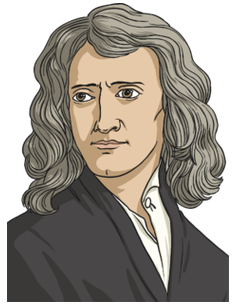
\includegraphics[width=.16\textwidth]{sir-isaac-newton}\\
			\text{\ak លោក អុីសាក់ ញូតុន}\\
			\text{(១៦៤២-១៧២៧)}
		\end{wrapfigure}
		\quad លោក អ៊ីសាក់ ញូតុន{\en (Isaac Newton)} ជាអ្នកវិទ្យាសាស្ត្រ និងជាអ្នកគណិតវិទ្យាដ៏ល្បីល្បាញម្នាក់។ នៅថ្ងៃទី ២៥ ខែធ្នូ ឆ្នាំ ១៦៤២  ឆ្នាំតែមួយ​ដែល​កាលីលេ​ទទួលមរណភាព​នៅ​អ៊ីតាលី អ្ន​កប្រាជ្ញ​មួយរូបទៀត​បាន​ចាប់កំណើតឡើង នៅ​ក្នុង​ប្រទេស​អង់គ្លេស... អ៊ីសាក់ ញូតុន ​ចាប់កំណើតឡើង​នៅ​ក្នុង​កាលៈទេសៈ​ដ៏លំបាក​មួយ ទាំង​នៅ​ក្នុង​គ្រួសារ និង​នៅ​ក្នុង​ប្រទេស។\\
		ញូតុន​​ចាប់កំណើត​ឡើង​​​ជា​កូនកំព្រា​ឪពុក។ ឪពុក​របស់​ញូតុន​​បាន​ទទួលមរណភាព​ តាំង​ពី ៣ខែមុន​ញូតុន​កើត ហើយ​នៅពេល​ដែល​ញូតុន​មាន​អាយុ​ទើប​នឹង​បាន ៣ឆ្នាំ ម្តាយ​បាន​រៀបការ​ប្តីថ្មី ហើយ​ទុកចោល​​ញូតុន​ឲ្យ​រស់នៅ​ជាមួយ​នឹង​ជីដូនជីតា ដោយសារ​តែ​ប្តីថ្មី​មិនចង់​ឲ្យ​ញូតុន​ទៅ​រស់នៅ​ជាមួយ។\\
		គាត់បានរៀន នៅ {\en Free Grammar School} និងបន្តទៅ {\en Trinity College, University of Cambridge}។ ពេលកំពុងរៀននៅអនុវិទ្យាល័យ គាត់បានចាប់អារម្មណ៍នឹងមុខវិជ្ជា គណិតវិទ្យា រូបវិទ្យា និងតារាសាស្រ្ត។ លោកញូតុន បានស្លាប់ នៅឆ្នាំ ១៧២៧  ពេលដែលគាត់មានអាយុ ៨៥ឆ្នាំ។
\end{biography}
\section{កម្លាំង}
\subsection{សញ្ញាណកម្លាំង{\en(Force Notation)}}
\begin{definition}
	\emph{\kml កម្លាំង} ជាបុព្វហេតុ៖
	\begin{itemize}
		\item [$-$] ធ្វើឲ្យអង្គធាតុមានចលនា ឬបម្រុងមានចលនា
		\item [$-$] បញ្ឈប់ ឬផ្លាស់ប្តូរទិសដៅចលនារបស់អង្គធាតុ
		\item [$-$] ធ្វើឲ្យអង្គធាតុខូចទ្រង់ទ្រាយ។
	\end{itemize}
\end{definition}
	\begin{enumerate}
		\item \emph{\kml កម្លាំង{\en(Force)}} ជាទំហំវ៉ិចទ័រដែលតាងដោយអក្សរ $\overrightarrow{F}$ ដូចនេះវាមានលក្ខណៈសម្គាល់បួនយ៉ាងគឺ ចំណុចចាប់ ទិស ទិសដៅ និងម៉ូឌុល ឬអាំងតង់ស៊ីតេ។
		\item \emph{\kml ខ្នាត់នៃកម្លាំង{\en(Unit of Force)}} ក្នុងប្រព័ន្ធខ្នាតអន្តរជាតិ $\left(\si{SI}\right)$ កម្លាំងមានខ្នាតគិតជា ញូតុន$\left(\si{\newton}\right)$។\\
		ឧបករណ៍សម្រាប់វាស់កម្លាំងគឺ ជញ្ជីងរ៉ឺស័រ ឬឌីណាម៉ូម៉ែត្រ។
		\begin{flalign*}
			\text{ខ្នាតកម្លាំង}\quad :&\quad 1\si{\newton}=\left(1\si{\kilogram}\right)\left(1\si{\meter/\second^{2}}\right)
		\end{flalign*}
		\item គេបានបែងចែកកម្លាំងជាពីរប្រភេទគឺ៖	
		\begin{enumerate}
			\item \emph{\kml កម្លាំងប៉ះ} ជាកម្លាំងដែលអង្គធាតុមួយបញ្ចេញលើអង្គធាតុមួយទៀត ដោយប៉ះគ្នាផ្ទាល់។ ឧទាហរណ៍ កម្លាំងទាញរ៉ឺស័រ កម្លាំងទាញរទេះ កម្លាំងទាត់បាល់។
			\begin{figure}[H]
				\centering
				\begin{subfigure}[b]{0.3\textwidth}
					\centering
					\begin{tikzpicture}
					\node at (0,0) {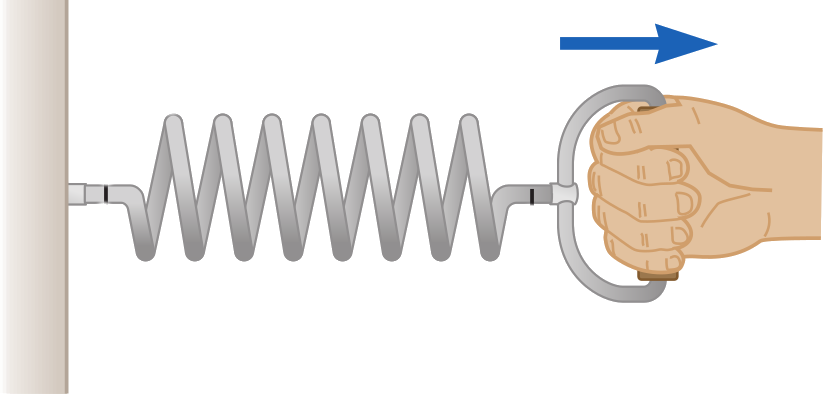
\includegraphics[scale=.18]{push_spring}};
					\draw[dashed] (-1.94,-.5)--(.76,-.5)--(.76,.6)--(-1.94,.6)--cycle;
					\end{tikzpicture}
					\caption{កម្លាំងទាញរ៉ឺស័រ}
				\end{subfigure}
				\begin{subfigure}[b]{0.3\textwidth}
					\centering
					\begin{tikzpicture}
					\node at (0,0) {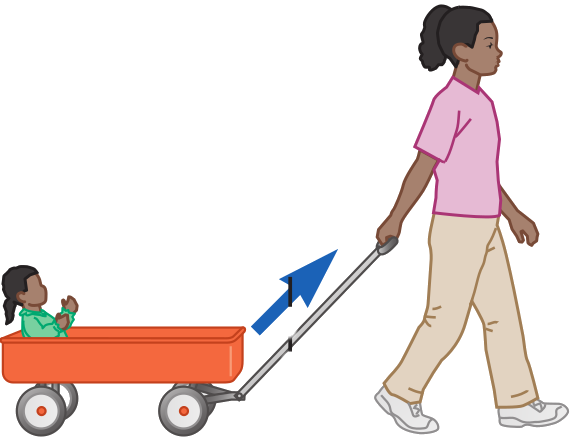
\includegraphics[scale=.25]{push_cart}};
					\draw[dashed] (-2.8,-2)--(1/20,-2)--(1/20,-.2)--(-2.8,-.2)--cycle;
					\end{tikzpicture}
					\caption{កម្លាំងទាញរទេះ}
				\end{subfigure}
				\begin{subfigure}[b]{0.3\textwidth}
					\centering
					\begin{tikzpicture}
					\node at (0,0) {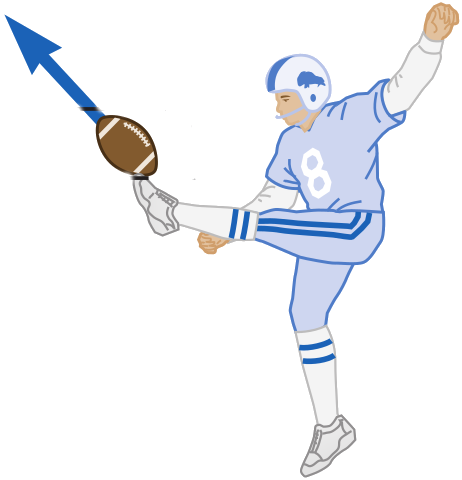
\includegraphics[scale=.25]{kick_ball}};
					\draw[dashed] (-1.5,.55)--(-.4,.55)--(-.4,1.15)--(-1.5,1.15)--cycle;
					\end{tikzpicture}
					\caption{កម្លាំងទាត់បាល់}
				\end{subfigure}
			\end{figure}
			\item \emph{\kml កម្លាំងពីចម្ងាយ ឬកម្លាំងដែន} ជាកម្លាំងដែលអង្គធាតុមួយបញ្ចេញលើអង្គធាតុមួយទៀត ដោយមិនចាំបាច់ប៉ះគ្នាផ្ទាល់។ ឧទាហរណ៍ កម្លាំងទំនាញផែនដី និងព្រះច័ន្ទ កម្លាំងអន្តរកម្មរវាងបន្ទុកអគ្គិសនីពីរដែលមានសញ្ញាដូចគ្នា ឬផ្ទុយគ្នា កម្លាំងឆក់ទាញដែកនៃមេដែក ជាដើម។ល។
			\begin{figure}[H]
				\centering
				\begin{subfigure}[b]{0.35\textwidth}
					\centering
					\begin{tikzpicture}
					\node at (0,0) {
\includegraphics[scale=.18]{earth}};
					\node at (-3,0) {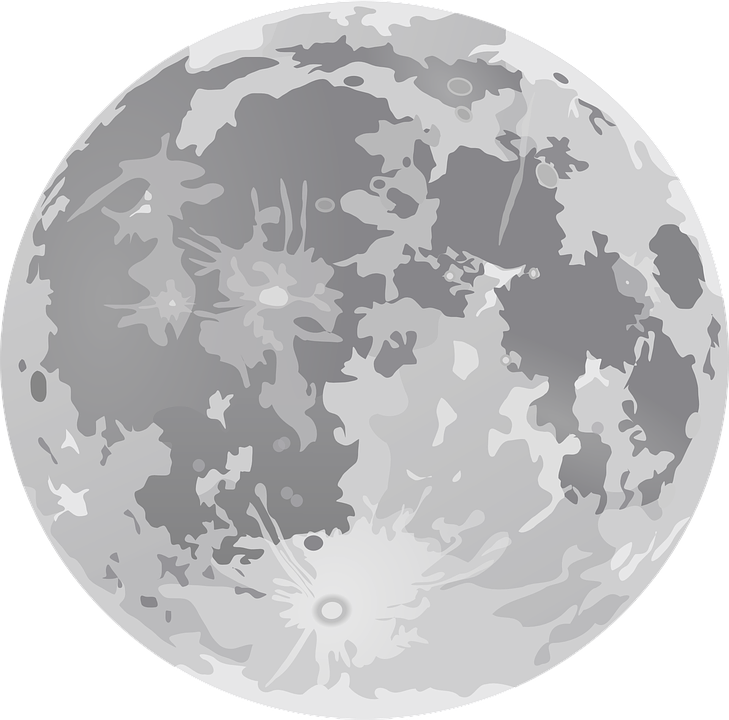
\includegraphics[scale=0.04]{moon}};
					\node at (0,-1.1) {$M_{\text{ផែនដី}}=5.9722\times10^{24}\si{\kilogram}$};
					\draw[dashed] (-3.7,-.6)--(-2.3,-.6)--(-2.3,.6)--(-3.7,.6)--cycle;
					\draw[->, line width=2pt, blue] (-2.5,0)--(-1.3,0);
					\node at (-1,1) {$M_{\text{ព្រះច័ន្ទ}}=7.342\times10^{22}\si{\kilogram}$};
					\end{tikzpicture}
					\caption{កម្លាំងទំនាញផែនដី និងព្រះច័ន្ទ}
				\end{subfigure}
				\begin{subfigure}[b]{0.32\textwidth}
					\centering
					\begin{tikzpicture}
						\shade[ball color = cyan!60!white, opacity = 0.8] (-2,0) circle (.5cm);
						\node at (-2,0) {$-q$};
						\shade[ball color = red!50!white, opacity = 0.8] (1,0) circle (1cm);
						\node at (1,0) {$+Q$};
						\draw[->, line width=2pt, blue] (-1.5,0)--(-.5,0);
						\node at (-2,0) {$-q$};
						\draw[dashed] (-2.8,-.6)--(-1.3,-.6)--(-1.3,.6)--(-2.8,.6)--cycle;
					\end{tikzpicture}
					\caption{កម្លាំងអន្តរកម្មបន្ទុកអគ្គិសនីពីរ}
				\end{subfigure}
				\begin{subfigure}[b]{0.3\textwidth}
					\centering
					\begin{tikzpicture}
					\node at (0,0) {
\includegraphics[scale=.25]{magetic_bar}};
					\draw[dashed]
					 (-3.2,-.8)--(-.7,-.8)--(-.7,.7)--(-3.2,.7)--cycle;
					 \node at (-2.2,-.2) {\large\text{\kml ដែក}};
					\end{tikzpicture}
					\caption{កម្លាំងឆក់ទាញដែកនៃមេដែក}
				\end{subfigure}
			\end{figure}
		\end{enumerate}
	\end{enumerate}
\begin{exercise}
	\begin{enumerate}
		\item គេមានវ៉ិចទ័រកម្លាំងពីរដែលមានប្រវែង $4\si{\centi\metre}$ និង $9\si{\centi\metre}$។ តើកម្លាំងនីមួយៗ មានអាំងតង់ស៊ីតេប៉ុន្មាន?\\ បើគេយកមាត្រដ្ឋាន $2\si{\centi\metre}$ ត្រូវនឹង $30\si{\newton}$។
		\item ម៉ាស៊ីនស្ទូចមួយបានស្ទូចវត្ថុមួយមានទម្ងន់ $8000\si{\newton}$ ដោយល្បឿនថេរតាមរយខ្សែឈរ។\\ ចូរតាងកម្លាំងដែលម៉ាស៊ីនស្ទូចមានអំពើលើវត្ថុនោះដោយវ៉ិចទ័រតាមមាត្រដ្ឋាន $1\si{\centi\metre}$ ត្រូវនឹង $2000\si{\newton}$។
		\item កម្លាំងទាញលើក្បាលរទេះភ្លើងនៅផ្លូវដែកមួយស្មើនឹង $30000\si{\newton}$ និងកម្លាំងទប់លើរទេះភ្លើងស្មើនឹង $10000\si{\newton}$។\\ ចូរតាងកម្លាំងនោះដោយវ៉ិចទ័រតាមមាត្រដ្ឋាន $1\si{\centi\metre}$ ត្រូវនឹង $10000\si{\newton}$។
	\end{enumerate}
\end{exercise}
\subsection{ផលបូកកម្លាំង}
	\begin{enumerate}[k]
		\item \emph{\kml ករណីកម្លាំងទាំងពីរមានទិសដៅដូចគ្នា}
		បើយើងមានវ៉ិចទ័រកម្លាំងពីរគឺ $\overrightarrow{F}_{1}$ និង $\overrightarrow{F}_{2}$ មានទិស និងទិសដៅដូចគ្នា។ \\គេបានកម្លាំងផ្គួបនៃកម្លាំងទាំងពីរគឺ $ \overrightarrow{F}=\overrightarrow{F}_{1}+\overrightarrow{F}_{2}$
		លក្ខណៈសម្គាល់នៃកម្លាំងផ្គួប $\overrightarrow{F}$ គឺ៖
		\begin{flalign*}
			\text{ចំណុចចាប់}\quad :&\quad\text{នៅត្រង់}~O\\
			\text{ទិស}\quad :&\quad \text{ស្របគ្នា}\\
			\text{ទិសដៅ}\quad :&\quad \text{ដូចទិសដៅរបស់} \overrightarrow{F}_{1}~\text{និង}~ \overrightarrow{F}_{2}\\
			\text{អាំងតង់ស៊ីតេ}\quad :&\quad F=F_{1}+F_{2}
		\end{flalign*}
		\begin{figure}[H]
			\centering
			\begin{tikzpicture}
			\begin{scope}[very thick, every node/.style={sloped,allow upside down}]
			\coordinate[label=left:$O$] (O) at (0,2);
			\coordinate (A) at (3,2);
			\coordinate[label=left:$O$] (B) at (0,1);
			\coordinate (C) at (2,1);
			\coordinate (D) at (5,0);
			\draw [->] (O) -- (A);
			\draw [->] (B) -- (C);
			\draw [->] (0,0) -- (D);
			\draw [arrows = {-Latex[width=6.5pt, length=6.5pt]}] (2.8,0) -- (3,0);
			\draw (-.3,0) node {$O$};
			\draw (-.3,-.5) node {$O$};
			\draw (1.2,2.4) node {$\overrightarrow{F}_{1}$};
			\draw (2,1.4) node {$\overrightarrow{F}_{2}$};
			\draw (2,.5) node {$\overrightarrow{F}_{1}$};
			\draw (4.5,.5) node {$\overrightarrow{F}_{2}$};
			\draw [->] (0,-.5) -- (5,-.5);
			\draw (5.2,-.5) node {$\overrightarrow{F}$};
			\end{scope}
			\end{tikzpicture}
			\caption{ផលបូកវុិចទ័រក​​​ម្លាំង​​ពីរមានទិស និងទិសដៅដូចគ្នា}
		\end{figure}
		\item \emph{\kml ករណីកម្លាំងទាំងពីរមានទិសដៅផ្ទុយគ្នា}
		បើយើងមានវ៉ិចទ័រកម្លាំងពីរគឺ $\overrightarrow{F}_{1}$ និង $\overrightarrow{F}_{2}$ មានទិសដៅផ្ទុយគ្នា។ \\គេបានកម្លាំងផ្គួបនៃកម្លាំងទាំងពីរគឺ $ \overrightarrow{F}=\overrightarrow{F}_{1}+\overrightarrow{F}_{2}$
		លក្ខណៈសម្គាល់នៃកម្លាំងផ្គួប $\overrightarrow{F}$ គឺ៖
		\begin{flalign*}
			\text{ចំណុចចាប់}\quad :&\quad\text{នៅត្រង់}~O\\
			\text{ទិស}\quad :&\quad \text{ស្របគ្នា}\\
			\text{ទិសដៅ}\quad :&\quad \text{មានទិសដៅដូច}\\ 
			\quad:&\quad\overrightarrow{F}_{1}~\text{បើ}~F_{1}>F_{2}~\text{នោះ}~F=F_{1}-F_{2}\\
			\quad:&\quad\overrightarrow{F}_{2}~\text{បើ}~F_{1}<F_{2}~\text{នោះ}~F=F_{2}-F_{1}\\
			\text{អាំងតង់ស៊ីតេ}\quad :&\quad F=\abs{F_{1}-F_{2}}
		\end{flalign*}
		\begin{figure}[H]
			\centering
			\begin{tikzpicture}
				\coordinate[label=above:$O$] (O1) at (0,0);
				\coordinate[label=above:$O$] (O2) at (0,-1);
				\coordinate[label=above:$\overrightarrow{F}$] (F) at (1,-1);
				\coordinate[label=above:$\overrightarrow{F}_{1}$] (A) at (3,0);
				\coordinate[label=above:$\overrightarrow{F}_{2}$] (B) at (-2,0);
				\draw[->] (O1)--(A);
				\draw[->] (O1)--(B);
				\node at (O1) {$\bullet$};
				\node at (0,-1) {$\bullet$};
				\draw[->] (O2) -- (F);
				\draw[dashed] (O2) -- (-1,-1);
			\end{tikzpicture}
			\caption{ផលបូកវុិចទ័រក​​​ម្លាំង​​ពីរមានទិសដៅផ្ទុយគ្នា ករណី $F_{1}>F_{2}$}
		\end{figure}
		\begin{figure}[H]
			\centering
			\begin{tikzpicture}
			\coordinate[label=above:$O$] (O1) at (0,0);
			\coordinate[label=above:$O$] (O2) at (0,-1);
			\coordinate[label=above:$\overrightarrow{F}$] (F) at (-1,-1);
			\coordinate[label=above:$\overrightarrow{F}_{1}$] (A) at (2,0);
			\coordinate[label=above:$\overrightarrow{F}_{2}$] (B) at (-3,0);
			\draw[->] (O1)--(A);
			\draw[->] (O1)--(B);
			\node at (O1) {$\bullet$};
			\node at (0,-1) {$\bullet$};
			\draw[->] (O2) -- (F);
			\draw[dashed] (O2) -- (1,-1);
			\end{tikzpicture}
			\caption{ផលបូកវុិចទ័រក​​​ម្លាំង​​ពីរមានទិសដៅផ្ទុយគ្នា ករណី $F_{1}<F_{2}$}
		\end{figure}
		\item \emph{\kml ករណីកម្លាំងទាំងពីរមានទិសដៅកែងគ្នា} បើយើងមានវ៉ិចទ័រកម្លាំងពីរគឺ $\overrightarrow{F}_{1}$ និង $\overrightarrow{F}_{2}$ មានទិស និងទិសដៅកែងគ្នា។ \\គេបានកម្លាំងផ្គួបនៃកម្លាំងទាំងពីរគឺ $ \overrightarrow{F}=\overrightarrow{F}_{1}+\overrightarrow{F}_{2}$
		លក្ខណៈសម្គាល់នៃកម្លាំងផ្គួប $\overrightarrow{F}$ គឺ៖
		\begin{flalign*}
			\text{ចំណុចចាប់}\quad :&\quad\text{នៅត្រង់}~O\\
			\text{ទិស}\quad :&\quad \text{ស្ថិតលើអង្កត់ទ្រូងនៃចតុកោណកែង}\\
			\text{ទិសដៅ}\quad :&\quad \text{មានទិសដៅដូចរូបខាងក្រោម}\\
			\text{អាំងតង់ស៊ីតេ}\quad :&\quad F=\sqrt{F^2_{1}+F^2_{2}}
		\end{flalign*}
		\begin{figure}[H]
			\centering
			\begin{tikzpicture}
			\begin{scope}
			\coordinate[label=below:$O$] (O) at (0,0);
			\coordinate (F1) at (2,0);
			\coordinate (F2) at (0,2);
			\coordinate (F) at (2,2);
			\draw [->] (O) -- (F1);
			\draw [->] (O) -- (F2);
			\draw [->] (O) -- (F);
			\draw [dashed] (0,2) --(2,2) -- (2,0);
			\coordinate[label=below:$\overrightarrow{F}_{1}$] (F1) at (F1);
			\coordinate[label=left:$\overrightarrow{F}_{2}$] (F2) at (F2);
			\coordinate[label=above:$\overrightarrow{F}$] (F) at (F);
			\pic [draw, -, "$\theta$", angle eccentricity=1.5] {angle = F1--O--F};
			\end{scope}
			\end{tikzpicture}
			\caption{ផលបូកវុិចទ័រ​​កម្លាំង​​ពីរមានទិស និងទិសដៅកែងគ្នា}
		\end{figure}
		\item \emph{\kml ករណីកម្លាំងទាំងពីរមានទិសបង្កើតបានមុំ $\theta$} 
		បើយើងមានវ៉ិចទ័រកម្លាំងពីរគឺ $\overrightarrow{F}_{1}$ និង $\overrightarrow{F}_{2}$ មានទិស និងទិសដៅបង្កើតបានមុំ $\theta$ មួយ។ គេបានកម្លាំងផ្គួបនៃកម្លាំងទាំងពីរគឺ $ \overrightarrow{F}=\overrightarrow{F}_{1}+\overrightarrow{F}_{2}$
		លក្ខណៈសម្គាល់នៃកម្លាំងផ្គួប $\overrightarrow{F}$ គឺ៖
		\begin{flalign*}
		\text{ចំណុចចាប់}\quad :&\quad\text{នៅត្រង់}~O\\
		\text{ទិស}\quad :&\quad \text{ស្ថិតលើអង្កត់ទ្រូងនៃប្រលេឡូក្រាម}\\
		\text{ទិសដៅ}\quad :&\quad \text{មានទិសដៅដូចរូបខាងក្រោម}\\
		\text{អាំងតង់ស៊ីតេ}\quad :&\quad F=\sqrt{F^2_{1}+F^2_{2}-2F_{1}F_{2}\cos\left(\pi-\theta\right)}\\
		\text{ឬ}\quad :&\quad F =\sqrt{F^2_{1}+F^2_{2}+2F_{1}F_{2}\cos\theta}
		\end{flalign*}
		\begin{figure}[H]
			\centering
			\begin{tikzpicture}
			\begin{scope}
			\coordinate[label=below:$O$] (O) at (0,0);
			\coordinate (01) at (2,0);
			\coordinate (F3) at (4,2);
			\coordinate (F1) at (2,2);
			\coordinate (F2) at (2,0);
			\coordinate (F) at (4,2);
			\draw [->] (O) -- (F1);
			\draw [->] (O) -- (F2);
			\draw [->] (O) -- (F);
			\draw [dashed] (2,2) --(4,2) -- (2,0);
			\coordinate[label=above:$\overrightarrow{F}_{1}$] (F1) at (F1);
			\coordinate[label=below:$\overrightarrow{F}_{2}$] (F2) at (F2);
			\coordinate[label=above:$\overrightarrow{F}$] (F) at (F);
			\pic [draw, -, "$\theta$", angle eccentricity=1.5] {angle = F2--O--F1};
			\end{scope}
			\end{tikzpicture}
			\caption{ផលបូកវុិចទ័រ​​កម្លាំង​​ពីរមានទិសបង្កើតបានមុំ $\theta$}
		\end{figure}
	\item \emph{\kml ករណីកម្លាំងច្រើនមានទិសជួបគ្នា}
		\begin{flalign*}
			\text{ផលបូកកម្លាំងរវាង $\overrightarrow{F}_{1}$ និង $\overrightarrow{F}_{2}$}\quad :&\quad \overrightarrow{F}=\overrightarrow{F}_{1}+\overrightarrow{F}_{2}\\
			\text{នោះ}\quad :&\quad \overrightarrow{R}=\overrightarrow{F}+\overrightarrow{F}_{3}\\
			\text{ឬ}\quad :&\quad \overrightarrow{R}=\overrightarrow{F}_{1}+\overrightarrow{F}_{2}+\overrightarrow{F}_{3}~\left(\overrightarrow{R}\text{ជាកម្លាំងផ្គួបនៃកម្លាំង} \overrightarrow{F}_{1},~\overrightarrow{F}_{2},~\overrightarrow{F}_{3}\right)
		\end{flalign*}
	\begin{figure}[H]
		\centering
		\begin{tikzpicture}
			\begin{scope}
				\coordinate[label=left:$O$] (O) at  (0,0);
				\coordinate[label=above:$\overrightarrow{F}_{1}$] (F1) at (2,1);
				\coordinate[label=below:$\overrightarrow{F}_{2}$] (F2) at (3,-.5);
				\coordinate[label=below:$\overrightarrow{F}_{3}$] (F3) at (4,-2);
				\coordinate[label=above:$\overrightarrow{F}$] (F) at (5,.7);
				\coordinate[label=above:$\overrightarrow{R}$] (R) at (9,-1);
				\draw[dashed] (F1) -- (F);
				\draw[dashed] (F2) -- (F);
				\draw[dashed] (F) -- (R);
				\draw[dashed] (F3) -- (R);
				\draw[->] (O) -- (F1);
				\draw[->] (O) -- (F2);
				\draw[->] (O) -- (F3);
				\draw[->] (O) -- (F);
				\draw[->, line width=2pt, magenta] (O) -- (R);
				\node at (O) {$\bullet$};
			\end{scope}
		\end{tikzpicture}
		\caption{ករណីមានវ៉ិចទ័រកម្លាំងច្រើនមានទិសជួបគ្នា}
	\end{figure}
	\end{enumerate}
	\begin{remark}
		ដើម្បីសង់វុិចទ័រកម្លាំងផ្គួប $\overrightarrow{F}$ ដែល $\overrightarrow{F}=\overrightarrow{F}_{1}+\overrightarrow{F}_{2}$ យើងត្រូវអនុវត្តតាមវិធានអង្តត់ទ្រូងប្រលេឡូក្រាម។
	\end{remark}
\begin{exercise}
	\begin{enumerate}[m]
		\item កម្លាំងខាងក្រោមនេះ ធ្វើអំពើលើចំណុចមួយនៃអង្គធាតុមួយ៖
		\begin{itemize}
			\item កម្លាំង $17\si{\newton}$ មានទិសឈរ និងមានទិសដៅពីក្រោមឡើងលើ
			\item កម្លាំង $11\si{\newton}$ មានទិសឈរ និងមានទិសដៅពីលើចុះក្រោម
			\item កម្លាំង $18\si{\newton}$ មានទិសដេក និងមានទិសដៅពីឆ្វេងទៅស្តាំ
			\item កម្លាំង $10\si{\newton}$ មានទិសដេក និងមានទិសដៅពីស្តាំទៅឆ្វេង។
		\end{itemize}
		រកកម្លាំងផ្គួបនៃកម្លាំងទាំងនោះ។
		\item កំណត់កម្លាំងផ្គួបនៃកម្លាំងពីរដែលមានអាំងតង់ស៊ីតេស្មើគ្នាហើយមុំបង្កើតដោយកម្លាំងទាំងពីរស្មើនឹង $60^{\circ}$។
		\item កំណត់កម្លាំងផ្គួបនៃកម្លាំងពីរដែលមានអាំងតង់ស៊ីតេស្មើគ្នា។\\ គេដឹងថាមុំដែលបង្កើតដោយកម្លាំងទាំងពីរស្មើនឹង $120^{\circ}$។
		\item កំណត់កម្លាំងផ្គួបនៃកម្លាំងជួបបីដែលមានអាំងតង់ស៊ីតេស្មើគ្នាឋិតក្នុងប្លង់តែមួយ ហើយបង្កើតបានមុំ $120^{\circ}$ ពីកម្លាំងមួយទៅកម្លាំងមួយទៀត(ដូចរូប)។
		\begin{figure}[H]
			\centering
			\begin{tikzpicture}[>=Stealth]
			\coordinate (O) at (0,0);
			\coordinate[label=below:$F_{1}$] (F1) at (0,-3);
			\coordinate[label=above:$F_{2}$] (F2) at (3, 1);
			\coordinate[label=above:$F_{3}$] (F3) at (-3, 1);
			\draw[->, magenta] (O)--(F1);
			\draw[->, magenta] (O)--(F2);
			\draw[->, magenta] (O)--(F3);
			\pic [draw, -, "$120^{\circ}$", angle eccentricity=2.5, angle radius=.3cm] {angle = F1--O--F2};
			\pic [draw, -, "$120^{\circ}$", angle eccentricity=2.5, angle radius=.3cm] {angle = F2--O--F3};
			\pic [draw, -, "$120^{\circ}$", angle eccentricity=2.5, angle radius=.3cm] {angle = F3--O--F1};
			\end{tikzpicture}
		\end{figure}
	\item ចូរគូសរូបដើម្បីរកកម្លាំងផ្គួបនៃកម្លាំងទាំងពីរគឺ $294\si{\newton}$ និង $392\si{\newton}$ ដែលបញ្ចេញលើអង្គធាតុមួយព្រមគ្នា និងមានទិសបង្កើតបានមុំ៖ $30^\circ,~60^\circ,~90^\circ$ និង $120^\circ$។ គណនាអាំងតង់ស៊ីតេនៃកម្លាំងផ្គួប។
	\end{enumerate}
\end{exercise}
\subsection{បំបែកកម្លាំង} កម្លាំងទោលមួយអាចបំបែកជាកម្លាំងផ្គុំពីរឬច្រើនដែលផ្តល់ផលដូចគ្នានឹងកម្លាំងទោលដោយប្រើវិធានប្រលេឡូក្រាម។
\begin{enumerate}
	\item \emph{\kml បំបែកកម្លាំងមួយជាកម្លាំងពីរកែងគ្នា}
	\begin{flalign*}
		\text{ជាវ៉ិចទ័រ}\quad :&\quad \overrightarrow{F}=\overrightarrow{F}_{x}+\overrightarrow{F}_{y}\\
		\text{ជាតម្លៃ}\quad :&\quad F=\sqrt{F^2_{x}+F^2_{y}}\quad
		\text{ដែល}\quad F_{x}=F\cos\theta~\text{និង}~F_{y}=F\sin\theta
	\end{flalign*}
	\begin{figure}[H]
		\centering
		\begin{tikzpicture}
		\begin{scope}
		\coordinate (O) at (0,0);
		\coordinate (x) at (3,0);
		\coordinate (y) at (0,3);
		\coordinate (F) at (2,2);
		\draw [->] (O) -- (x);
		\draw [->] (O) -- (y);
		\draw [->] (O) -- (F);
		\draw [dashed] (0,2) --(2,2) -- (2,0);
		\coordinate[label=below:$x$] (x) at (x);
		\coordinate[label=left:$y$] (y) at (y);
		\coordinate[label=above:$\overrightarrow{F}$] (F) at (F);
		\coordinate[label=below:$\overrightarrow{F}_{x}$] (Fx) at (2,0);
		\coordinate[label=left:$\overrightarrow{F}_{y}$] (Fy) at (0,2);
		\coordinate[label=below:$O$] (0,0) at (0,0);
		\pic [draw, -, "$\theta$", angle eccentricity=1.5] {angle = x--O--F};
		\end{scope}
		\end{tikzpicture}
		\caption{បំបែកកម្លាំងមួយជាកម្លាំងពីរកែងគ្នា}
	\end{figure}
	\item \emph{\kml បំបែកកម្លាំងមួយជាកម្លាំងពីរស្របគ្នា}
	\begin{figure}[H]
		\centering
		\begin{tikzpicture}
			\begin{scope}
				\draw[->] (.5,0)--(.5,-2);
				\draw[->] (7.5,0)--(7.5,-2);
				\fill[top color=gray, bottom color=gray!40!white] (0,0) rectangle (8,.3);
				\shade[bottom color=fancyorange1, top color=fancyorange2] (.5,0)--(-.5,-1)--(1.5,-1)--cycle;
				\shade[bottom color=fancyorange1, top color=fancyorange2] (7.5,0)--(8.5,-1)--(6.5,-1)--cycle;
				\shade[bottom color=fancyorange1, top color=fancyorange2] (5,.3)--(6,.3)--(6,1.5)--(5,1.5)--cycle;
				\node at (5.5,.8) {$\bullet$};
				\draw[->,line width=2pt] (5.5,.8)--(5.5,-2);
				\draw[<->] (.5,1)--(5,1);
				\draw[<->] (6,1)--(7.5,1);
				\node at (2.5,1.2) {$d_{1}$};
				\node at (6.7,1.2) {$d_{2}$};
				\node at (1,-1.8) {$\overrightarrow{F}_{1}$};
				\node at (6,-1.8) {$\overrightarrow{F}$};
				\node at (8,-1.8) {$\overrightarrow{F}_{2}$};
			\end{scope}
		\end{tikzpicture}
		\caption{បំបែកកម្លាំងមួយជាកម្លាំងពីរស្របគ្នា}
	\end{figure}
	\begin{flalign*}
		\text{ជាវ៉ិចទ័រ}\quad :&\quad \overrightarrow{F}=\overrightarrow{F}_{1}+\overrightarrow{F}_{2}\\
		\text{ជាម៉ូឌុល}\quad :&\quad F=F_{1} + F_{2}\\
		\text{ម្យ៉ាងទៀត}\quad :&\quad F_{1}\times d_{1}=F_{2}\times d_{2}~\text{ឬ}~\frac{F_{1}}{F_{2}}=\frac{d_{2}}{d_{1}}
	\end{flalign*}
\end{enumerate}
\begin{exercise}
	\begin{enumerate}
		\item កម្លាំង $10\si{\newton}$ មានទិសបង្កើតបាន $37^\circ$ ធៀបនឹងទិសដេក។ រកកម្លាំងផ្គុំឈរ និងកម្លាំងផ្គុំដេករបស់វា។
		\item គេដំដែកគោលមួយលើជញ្ជាំងតាមមុំ $45^\circ$ នឹងប្លង់ជញ្ជាំងឈរដោយកម្លាំង $30\si{\newton}$។\\
		រកអាំងតង់ស៊ីតេកម្លាំងផ្គុំតាមទិសដេក និងទិសឈរ។
	\end{enumerate}
\end{exercise}
\section{ច្បាប់ចលនារបស់ញូតុន}
\subsection{ច្បាប់ទី១ ញូតុន ឬ ច្បាប់និចលភាព}
\begin{itemize}
	\item \emph{\kml ច្បាប់ទី១ ញូតុនពោលថាៈ} កាលណាអង្គធាតុមួយមិនរងអំពើនៃកម្លាំងផ្សេងៗទេ ឬវារងកម្លាំងផ្គួបស្មើនឹងសូន្យ នោះបើវានៅនឹងថ្កល់ស្រាប់វានឹងនៅតែនឹងថ្កល់ដដែល តែបើវាមានចលនាស្រាប់ ចលនានោះជាចលនាត្រង់ស្មើ។
	\item \emph{\kml និចលភាព} ជាលក្ខណៈនៃគ្រប់អង្គធាតុដែលចង់រក្សាភាពមានចលនា ឬភាពនៅនឹងថ្កល់របស់វា។ គេអាចនិយាយម្យ៉ាងទៀតថា លក្ខណៈរក្សាល្បឿននៃអង្គធាតុហៅថា និចលភាព ហើយចលនាត្រង់ស្មើហៅថា ចលនាដោយនិចលភាព។
	\item \emph{\kml ច្បាប់ទី១ ញូតុន គេអាចសរសេរ} $\Sigma \overrightarrow{F}=\overrightarrow{0}$
\end{itemize}
\begin{remark}
	ក្នុងភាពលំនឹងមានន័យថា វត្ថុអាចនៅនឹងថ្កល់ ឬក៏កំពុងផ្លាស់ទីលើគន្លងត្រង់ដោយវ៉ិចទ័រល្បឿនថេរ(ចលនាត្រង់ស្មើ)។ លក្ខណៈបែបនេះ ហៅថានិចលភាព។
\end{remark}
\subsection{ច្បាប់ទី២ ញូតុន ឬ ច្បាប់គ្រឹះឌីណាមិច}
\begin{itemize}
	\item \emph{\kml ច្បាប់ទី២ ញូតុនពោលថាៈ} នៅពេលកម្លាំងសរុបដែលមានអំពើលើវត្ថុមួយមិនស្មើសូន្យ វត្ថុនឹងស្ទុះតាមទិសដៅកម្លំាងដែលបានប្រព្រឹត្តលើវា ហើយសំទុះសមាមាត្រដោយផ្ទាល់នឹងកម្លាំងសរុប ដែលមានអំពើលើវាហើយ ច្រាសសមាមាត្រនឹងម៉ាសរបស់វា។
	\begin{flalign*}
		\text{សំទុះនៃចលនារបស់អង្គធាតុសមាមាត្រនឹងកម្លាំងផ្គួប}\quad :&\quad \overrightarrow{a}\propto\Sigma \overrightarrow{F}\\
		\text{សំទុះនៃចលនារបស់អង្គធាតុច្រាសសមាមាត្រនឹងកម្លាំងផ្គួប}\quad :&\quad \overrightarrow{a}\propto\frac{1}{m}\\
		\text{គេបាន}\quad :&\quad \overrightarrow{a}=\frac{\Sigma \overrightarrow{F}}{m}~\text{ឬ}~\Sigma\overrightarrow{F}=m\overrightarrow{a}\\
		\text{ជាម៉ូឌុល}\quad :&\quad \Sigma F=ma~\left(\overrightarrow{F}~\text{និង}~\overrightarrow{a}~\text{មានទិសដៅដូចគ្នា}\right)
	\end{flalign*}
	\begin{remark}
		\begin{itemize}
			\item បើកម្លាំង $\overrightarrow{F}$ ថេរ នាំឲ្យសំទុះថេរ៖ អង្គធាតុមានចលនាត្រង់ប្រែប្រួលស្មើ។
			\item បើកម្លាំង $\overrightarrow{F}$ ថេរ និងមានទិសដៅដូចល្បឿន៖ អង្គធាតុមានចលនាត្រង់ស្ទុះស្មើ។
			\item បើកម្លាំង $\overrightarrow{F}$ ថេរ និងទិសដៅផ្ទុយពីល្បឿន៖ អង្គធាតុមានចលនាត្រង់យឺតស្មើ
			\item បើកម្លាំង $\overrightarrow{F}=\overrightarrow{0}$ និងមាន $\overrightarrow{a}=\overrightarrow{0}$៖ អង្គធាតុមានចលនាត្រង់ស្មើ។ 
		\end{itemize}
	\end{remark}
\end{itemize}
\begin{exercise}
	\begin{enumerate}
		\item ក្មេងប្រុសម្នាក់រុញប្រអប់មួយដែលមានម៉ាស $10\si{\kilogram}$ ដោយកម្លាំង $20\si{\newton}$។ តើសំទុះនៃប្រអប់ស្មើនឹងប៉ុន្មាន? កកិតអាចចោលបាន។
		\item រថយន្តមួយមានម៉ាស $1.0\times10^{3}\si{\kilogram}$ មានចលនាស្ទុះស្មើដោយចាប់ផ្តើមពីល្បឿនសូន្យទៅល្បឿន $20\si{\metre/\second}$ ក្នុងរយៈពេល $10\si{\second}$។ គណនាកម្លាំងម៉ាស៊ីនដែលរថយន្តបញ្ចេញដើម្បីឲ្យវាទៅមុខ។ កម្លាំងកកិតអាចចោលបាន។ 
		\item គណនាកម្លាំងចំបាច់ ដើម្បីឲ្យវត្ថុមួយមានម៉ាស $48\si{\kilogram}$ មានសំទុះ $6\si{\metre/\second^{2}}$។
		\item កម្លាំង $200\si{\gram\cdot\centi\metre/\second^{2}}$ បញ្ជូនសំទុះ $500\si{\centi\metre/\second^{2}}$ ឲ្យវត្ថុមួយ។ គណនាម៉ាសនៃវត្ថុនោះ។
		\item កម្លាំង $0.20\si{\newton}$ មានអំពើលើវត្ថុមួយដែលមានម៉ាស $100g$។ គណនាសំទុះនៃវត្ថុនោះ។
		\item កម្លាំង $\SI{e-2}{\newton}$ មានអំពើលើវត្ថុមួយដែលមានម៉ាស $1\si{\gram}$។\\ តើមួយវិនាទីក្រោយមក វត្ថុនោះផ្លាស់ទីបានចម្ងាយប៉ុន្មានម៉ែត្រ? តើ $5\si{\second}$ ក្រោមមកវាមានល្បឿនប៉ុន្មាន?
		\item កម្លាំងថេរមួយមានអំពើលើវត្ថុមួយមានម៉ាស $300\si{\gram}$ ធ្វើឲ្យវត្ថុនោះចេញពីស្ថានភាពនៅស្ងៀមហើយផ្លាស់ទីបានចម្ងាយ $25\si{\meter}$ ក្នុងរយៈពេល $5\si{\second}$។ គណនាកម្លាំងនោះ។
		\item កូនបាល់មួយមានម៉ាស $100\si{\gram}$ កំពុងឋិតនៅស្ងៀម ហើយរងកម្លាំងមួយថេរស្មើនឹង $200\si{\gram\cdot\centi\metre/\second^{2}}$ ក្នុងរយៈពេល $10\si{\second}$។ គណនាល្បឿនរបស់បាល់ និងចម្ងាយដែលវាផ្លាស់ទីបានក្នុងរយៈពេល $10\si{\second}$។
	\end{enumerate}
\end{exercise}
\subsection{ច្បាប់ទី៣ ញូតុន ឬ ច្បាប់អំពើ និងប្រតិកម្ម}
\begin{itemize}
	\item \emph{\kml ច្បាប់ទី៣ ញូតុនពោលថាៈ} នៅពេល វត្ថុទី១បញ្ចេញកម្លាំងមួយទៅលើវត្ថុទី២ នោះវត្ថុទី២ ក៏បញ្ចេញកម្លាំងមួយមកលើវត្ថុទី១ វិញដែរ ដែលមានតម្លៃស្មើគ្នា ប៉ុន្តែមានទិសដៅផ្ទុយគ្នា។
	\begin{flalign*}
		\text{កម្លាំងអំពើ~$\overrightarrow{F}_{12}$}\quad :&\quad \text{ជាកម្លាំងដែលវត្ថុទី១ បញ្ចេញលើវត្ថុទី២}\\
		\text{កម្លាំងប្រតិកម្ម~$\overrightarrow{F}_{21}$}\quad :&\quad \text{ជាកម្លាំងដែលវត្ថុទី២ បញ្ចេញលើវត្ថុទី១}
	\end{flalign*}
	\item \emph{\kml ច្បាប់ទី៣ ញូតុនបង្ហាញលក្ខណៈសម្គាល់បួនយ៉ាងនៃកម្លាំង មានដូចជា៖}
	\begin{itemize}
		\item [$-$] កម្លាំងកើតឡើងជាគូ។ គូកម្លាំងនេះហៅថា អំពើ និងប្រតិកម្ម។
		\item [$-$] អំពើ និងប្រតិកម្មមាន អាំងតង់ស៊ីតេស្មើគ្នា។
		\item [$-$] អំពើ និងប្រតិកម្មមានទិសដៅផ្ទុយគ្នា។
		\item [$-$] អំពើ និងប្រតិកម្មមានចំណុចចាប់លើអង្គធាតុពីរផ្សេងគ្នា ដូចនេះ វាមិនមែនជាកម្លាំងលំនឹងទេ។
	\end{itemize}
	\item \emph{\kml ច្បាប់ទី៣ ញូតុន គេអាចសរសេរ} $\overrightarrow{F}_{12}=-\overrightarrow{F}_{21}$ ជាតម្លៃ $F_{12}=F_{21}$
	\begin{figure}[H]
		\centering
		\begin{tikzpicture}
			\node at (0,0) {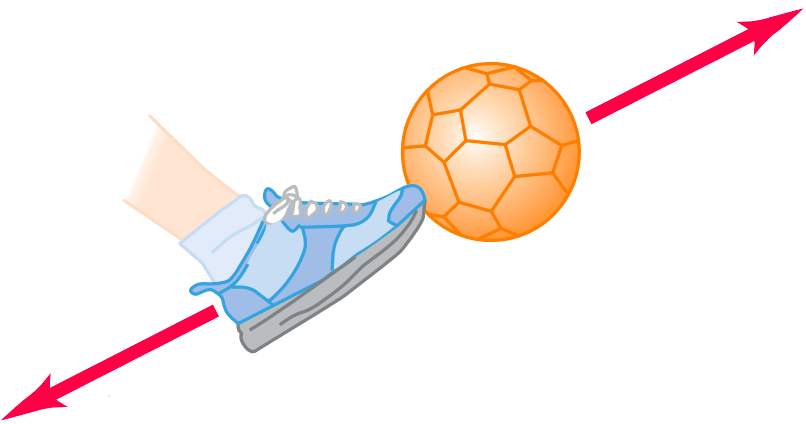
\includegraphics[scale=.2]{third_law_newton}};
			\node at (-2,-1.7) {$\vec{F}_{\text{បាល់មានអំពើលើជើង}}$};
			\node at (4,.8) {$\vec{F}_{\text{ជើងមានអំពើលើបាល់}}$};
		\end{tikzpicture}
		\caption{កម្លាំងជើងនិងបាល់បញ្ចេញអន្តរកម្មលើគ្នាទៅវិញទៅមក ដែលមានទំហំស្មើគ្នា ក្នុងទិសដៅផ្ទុយ}
	\end{figure}
\end{itemize}
\section{ម៉ាស និងទម្ងន់}
\subsection{ម៉ាស{\en(Mass)}}
\begin{definition}
	ម៉ាសនៃអង្គធាតុមួយ ជាទំហំអាស្រ័យតែនឹងអង្គធាតុនោះផ្ទាល់ ហើយមានឥទ្ធិពលដល់ទម្ងន់របស់អង្គធាតុនោះ។ អង្គធាតុមួយមានម៉ាសកំណត់។ បើម៉ាសនៃអង្គធាតុកាន់តែធំ នោះនិចលភាពនៃអង្គធាតុនោះ ក៏កាន់តែធំដែរ។ ដូចនេះ ម៉ាសជាទំហំកំណត់និចលភាពនៃវត្ថុ។
\end{definition}
\subsection{ទម្ងន់ ឬកម្លាំងទំនាញដែនដី{\en(Weight or Gravitational Force)}}
\begin{definition}
	 ទម្ងន់ ឬកម្លាំងទំនាញផែនដី ជាកម្លាំងដែលផែនដីទាញវត្ថុ ហើយមានទិសដៅតម្រង់មករកផ្ចិតនៃផែនដី។\\
	 ដើម្បីគណនាទម្ងន់នៃអង្គធាតុមួយ យើងប្រើរូបមន្ត $\vec{w}=m\vec{g}$ ជាម៉ូឌុល $w=mg$ ដែល $g$ ជាសំទុះទំនាញផែនដី។
\end{definition}
\begin{remark}
	\begin{enumerate}[k,2]
		\item ម៉ាសបង្ហាញពីបរិមាណរូបធាតុដែលបង្កើតវត្ថុ។
		\item ទម្ងន់បង្ហាញពីទំហំរបស់ទំនាញ។
	\end{enumerate}
\end{remark}
\subsection{ភាពខុសគ្នារវាង ម៉ាស និងទម្ងន់}
\begin{center}
	\begin{tabular}{|l|l|}
		\hline
		\multicolumn{1}{|c|}{{\cellcolor[HTML]{96FFFB}\ak ម៉ាស}} & \multicolumn{1}{|c|}{{\cellcolor[HTML]{96FFFB}\ak ទម្ងន់}}\\
		\hline
		- ជាបរិមាណរូបធាតុមាននៅក្នុងអង្គធាតុ & 	
		- ជាកម្លាំងទំនាញផែនដី \\ 
		- មានតែតម្លៃ គ្មានទិសដៅ & 
		- មានតម្លៃ និងទិសដៅ\\ 
		- មានខ្នាត់គិតជាគីឡូក្រាម $\left(\si{\kilogram}\right)$ &
		- មានខ្នាត់គិតជាញូតុន $\left(\si{\newton}\right)$\\
		- មានតម្លៃថេរគ្រប់ទីកន្លែង &
		- ប្រែប្រួលតាមទីកន្លែង\\
		- វាស់ដោយជញ្ជីង & 
		- វាស់ដោយឌីណាម៉ូម៉ែត្រ\\
		\hline
	\end{tabular}
\end{center}
\begin{figure}[H]
	\centering
	\begin{subfigure}[b]{0.45\textwidth}
		\centering
		\begin{tikzpicture}
			\node at (0,0) {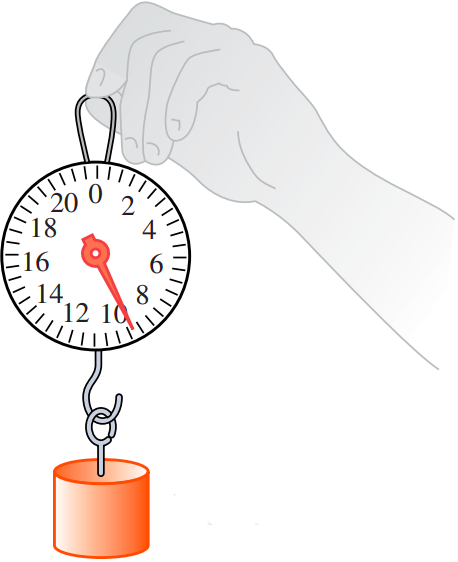
\includegraphics[scale=.25]{mass_on_earth}};
			\draw[->, line width=2pt, magenta] (-1.3,-2.4)--(-1.3,-4.5);
			\draw[->, line width=2pt, blue] (-1,-2.4)--(-1,-3.5);
			\node at (1,-2) {\text{ម៉ាស}~$m=1.00\si{\kilogram}$};
			\node at (1.5,-3) {\text{សំទុះទំនាញដី}~$g=9.80\si{\meter/\second^{2}}$};
			\node at (-3,-4) {\text{ទម្ងន់}~$w=9.80\si{\newton}$};
		\end{tikzpicture}
		\caption{ម៉ាស និងទម្ងន់របស់វត្ថុស្ថិតនៅលើផែនដី}
	\end{subfigure}
	\begin{subfigure}[b]{0.45\textwidth}
		\centering
		\begin{tikzpicture}
		\node at (0,0) {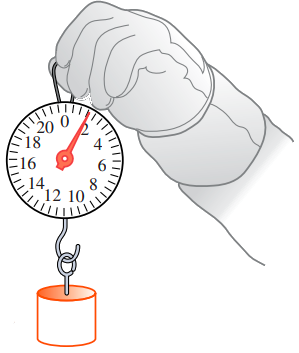
\includegraphics[scale=.35]{mass_on_the_moon}};
		\draw[->, line width=2pt, blue] (-.9,-2.1)--(-.9,-2.8);
		\draw[->, line width=2pt, magenta] (-1.2,-2.1)--(-1.2,-3);
		\node at (1,-1.8) {\text{ម៉ាស}~$m=1.00\si{\kilogram}$};
		\node at (1.8,-2.8) {\text{សំទុះទំនាញ}~$g=1.62\si{\meter/\second^{2}}$};
		\node at (-3,-3) {\text{ទម្ងន់}~$w=1.62\si{\newton}$};
		\end{tikzpicture}
		\caption{ម៉ាស និងទម្ងន់របស់វត្ថុស្ថិតនៅលើឋានព្រះច័ន្ទ}
	\end{subfigure}
\end{figure}
\begin{remark}
	ម៉ាសរបស់វត្ថុមួយមានតម្លៃថេរជានិច្ច ប៉ុន្តែទម្ងន់របស់វាប្រែប្រួលតាមទីកន្លែងដែលវាស្ថិតនៅ។
\end{remark}
\begin{exercise}
	\begin{enumerate}
		\item អង្គធាតុមួយមានទម្ងន់ $100\si{\newton}$ នៅលើផែនដី។ បើគេយកអង្គធាតុនោះទៅកាន់ភពមួយដែលមានសំទុះទំនាញស្មើនឹង $2\si{\metre/s^2}$។ តើអង្គធាតុនោះមានទម្ងន់ប៉ុន្មាននៅលើភពនោះ?
		\item នៅចុងខ្សែមួយបានចងភ្ជាប់នឹងកូនជញ្ជីង $50\si{\kilogram}$។ គេទាញកូនជញ្ជីងចេញពីទីតាំងលំនឹងបានមុំ $30^\circ$។\\ រកកម្លាំងដែលទាញកូនជញ្ជីងពីទីតាំងលំនឹង និងតំណឹងនៃខ្សែ។
		\begin{figure}[H]
			\centering
			\begin{tikzpicture}[>=stealth]
			\begin{scope}
				\coordinate (centre) at (0,0);
				\coordinate (force) at (3.5,-2.3);
				\draw[dashed,gray] (centre) -- ++ (0,-1) node (mary) [black,below]{$ $};
				\draw[magenta] (centre) -- ++(310:3) coordinate (block);
				\draw[->] (block)--(force) node[above] (force) {$\vec{F}$};
				\draw[<-, magenta, >=Latex] (310:1.5) -- (block);
				\draw[->, magenta, >=Latex] (1.9,-2.5) -- (1.9,-3.5) node[below] (1.9,-3.5) {$\vec{w}=m\vec{g}$};
				\node[circle,outer color=teal,inner color=white,minimum width=.8cm] (radial) at (block) {};
				\pic [draw, ->, "$30^\circ$", angle eccentricity=1.5, angle radius=1cm] {angle = mary--centre--block};
				\draw [line width=2pt] (-.6,0) -- (.6,0);
				\fill[bottom color=gray, top color=gray!40!white] ($ (centre) + (-.6,0) $) rectangle ($ (centre) + (.6,0.2) $);
				\coordinate (m) at (block);
				\node at (1.3,-1) {$\vec{T}$};
			\end{scope}
			\end{tikzpicture}
		\end{figure}
	\item តំណក់ទឹកភ្លៀងជាមធ្យមមានម៉ាស $0.05\si{\gram}$។ ដោយសារខ្យល់បក់តាមទិសដេក ទើបតំណក់ទឹកភ្លៀងធ្លាក់ចុះមកដីតាមទិសដែលធ្វើបានមុំ $60^\circ$ ជាមួយប្លង់ដេក។ រកកម្លាំងខ្យល់បក់លើតំណក់ទឹកភ្លៀង។
	\item គេព្យួរវត្ថុមួយដែលមានម៉ាស $60\si{\kilogram}$ ទៅនឹងចុងខ្សែពីរដែលទិសវាបង្កើតបានមុំ $ABC$ ស្មើនឹង $120^\circ$(ដូចរូប)។\\ រកតំណឹងនៃខ្សែទាំងពីរគឺខ្សែ $AB$ និងខ្សែ $BC$។
	\begin{figure}[H]
		\centering
		\begin{tikzpicture}[>=stealth, decoration=rope]
		\begin{scope}
		\coordinate[label=below left:{$A$}] (A) at (0,0);
		\coordinate[label=below left:{$B$}] (B) at (2,-2);
		\coordinate[label=below left:{$C$}] (C) at (4,-2);
		\coordinate (T1) at (1.8,-1);
		\coordinate (block) at (2,-2.5);
		\draw[gray,thin,decorate,rope width=3pt] (A) -- (B);
		\draw[gray,thin,decorate,rope width=3pt] (B) -- (C);
		\draw[gray,thin,decorate,rope width=3pt] (B) -- (block);
		\node at (A) {$\bullet$};
		\node at (B) {$\bullet$};
		\node at (C) {$\bullet$};
		\node[circle,outer color=gray,inner color=white,minimum width=.1cm] (radial) at (B) {};
%		\coordinate[label=above:{$\vec{T}_{BC}$}] (T2) at (3,-2);
		\fill[bottom color=gray, top color=gray!40!white] ($ (A) + (-.6,0) $) rectangle ($ (A) + (.6,0.3) $);
		\fill[left color=gray, right color=gray!40!white] ($ (C) + (0,-.5) $) rectangle ($ (C) + (.3,.5) $);
%		\node at (T1) {$\vec{T}_{AB}$};
		\node at (block) {$\bullet$};
		\shade[top color=teal,bottom color=teal,middle color=white, fill opacity=1.0, rounded corners] (1.5,-3.5) rectangle (2.5,-2.5);
		\pic [draw, ->, "$120^\circ$", angle eccentricity=1.5, angle radius=.5cm] {angle = C--B--A};
		\node at (2,-3) {$60\si{\kilogram}$};
		\end{scope}
		\end{tikzpicture}
	\end{figure}
	\end{enumerate}
\end{exercise}
\section{កម្លាំងកែង និងកម្លាំងកកិត}
\subsection{កម្លាំងកែង ឬកម្លាំងប្រតិកម្មកែង{\en (Normal Force)}}
\quad មុនយើងនិយាយពីកម្លាំងកកិត យើងនឹងរៀនអំពីកម្លាំងថ្មីមួយទៀត ហៅថាកម្លាំងកែង។ កម្លាំងកែង មានអំពើលើវត្ថុដែលប៉ះនឹងផ្ទៃ។ វាមានអំពើកែងជានិច្ចនឹងផ្ទៃប៉ះ។ គេតាងវ៉ិចទ័រកម្លាំងកែងដោយ $\vec{F}_{N}$
\begin{figure}[H]
	\centering
	\begin{subfigure}[b]{0.4\textwidth}
		\centering
		\begin{tikzpicture}
		\node at (0,0) {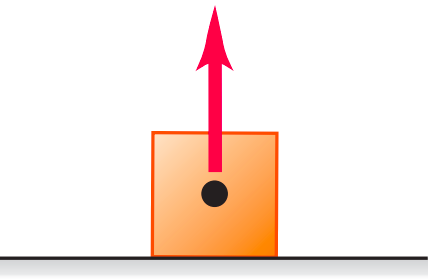
\includegraphics[scale=.2]{normal_force1}};
		\node at (.4,1) {$\vec{F}_{N}$};
		\end{tikzpicture}
		\caption{កម្លាំងកែងលើប្លង់ដេក}
	\end{subfigure}
	\begin{subfigure}[b]{0.4\textwidth}
		\centering
		\begin{tikzpicture}
		\node at (0,0) {
\includegraphics[scale=.2]{normal_force2}};
		\node at (1.4,1) {$\vec{F}_{N}$};
		\end{tikzpicture}
		\caption{កម្លាំងកែងលើប្លង់ទេរ}
	\end{subfigure}
\end{figure}
\begin{flalign*}
	\text{រូបមន្តដើម្បីគណនាកម្លាំងកែងគឺ}\quad :&\quad \vec{F}_{N}=-\vec{w}=-m\vec{g}~\text{(ប្លង់ដេក)}\\
	\text{ជាម៉ូឌុល}\quad :&\quad F_{N}=w=mg\\
\end{flalign*}
\subsection{កម្លាំងកកិត​{\en (Friction Forces)}}
\quad ឥឡូវ យើងនឹងនិយាយអំពីកកិត។ ឧបមាថាយើងរុញសៀវភៅមួយក្បាលក្រោមល្បឿនថេរ ដោយកម្លាំង $\vec{F}$ លើផ្ទៃតុមួយ នោះយើងនឹងសង្កេតឃើញថាកកិតរវាងផ្ទៃតុ នឹងសៀវភៅកើតមានឡើង។ កម្លាំងដែលកើតឡើងដោយសារកកិតរវាងវត្ថុពីរនោះហៅថាកម្លាំងកកិតដែលតាងដោយ $\vec{f}$ ហើយមានទិសដៅផ្ទុយនឹងកម្លាំងដែលកំពុងរុញសៀវភៅនោះគឺ $\vec{F}$។
\begin{figure}[H]
	\centering
	\begin{tikzpicture}
		\node at (0,0) {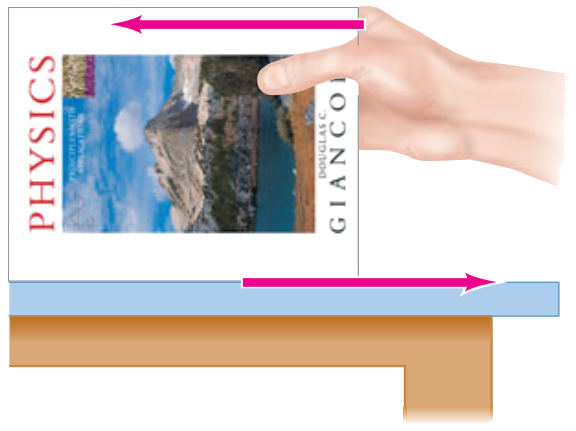
\includegraphics[scale=.3]{push_book}};
		\node at (-1.5,2.5) {$\vec{F}$};
		\node at (2,-.2) {$\vec{f}$};
	\end{tikzpicture}
	\caption{កម្លាំងកកិត}
\end{figure}
\begin{definition}
	កម្លាំងកកិត ជាកម្លាំងដែលកើតមានឡើងនៅត្រង់ផ្ទៃប៉ះគ្នារវាងវត្ថុពីរ។ យើងតាងវ៉ិចទ័រកម្លាំងកកិតដោយ $\vec{f}$។\\
	កម្លាំងកកិតមានពីរប្រភេទគឺ
	\begin{itemize}
		\item កកិតស្តាទិច{\en(Static Friction)}\quad: ជាកកិតដែលកើតមានឡើង កាលណាកម្លាំងទប់(កម្លាំងកកិត) និងកម្លាំងបញ្ចេញលើវត្ថុមួយ ធ្វើឲ្យអង្គធាតុនោះនៅនឹងថ្កល់។ កកិតស្តាទិចអាចហៅថា កកិតនឹងថ្កល់។\\ គេតាងកម្លាំងកកិតស្តាទិចដោយ $f_{s}$។
		\item កកិតស៊ីនេទិច{\en(Kinetic Friction)}\quad: ជាកកិតដែលកើតមានឡើងកាលណាវត្ថុមានចលនា ហើយវាប្រឆាំងនឹងទិសដៅនៃបម្លាស់ទីរបស់វត្ថុ។ កកិតស៊ីនេទិចមានពីរប្រភេទគឺ កកិតដោយរអិល និងកកិតដោយរមៀល។\\ គេតាងកម្លាំងកកិតស៊ីនេទិចដោយ $f_{k}$។
	\end{itemize}
\end{definition}
\begin{formula}
	មេគុណកកិត ជាផលធៀបរវាងកម្លាំងកកិត នឹងកម្លាំងកែង។
	\begin{flalign*}
		\text{គេសរសេរ}\quad :&\quad \text{មេគុណកកិត $\left(\mu\right)$}=\frac{\text{កម្លាំងកកិត $\left(f\right)$}}{\text{កម្លាំងកែង} \left(F_{N}\right)}\\
		\text{កម្លាំងកកិតស្តាទិច}\quad :&\quad f_{s}=\mu_{s}F_{N}~\text{ដែល}~ \mu_{s}~\text{ជាមេគុណកកិតស្តាទិច}\\
		\text{កម្លាំងកកិតស៊ីនេទិច}\quad :&\quad f_{k}=\mu_{k}F_{N}~\text{ដែល}~ \mu_{k}~\text{ជាមេគុណកកិតស៊ីនេទិច}
	\end{flalign*}
\end{formula}
\begin{figure}[H]
	\centering
	\begin{tikzpicture}
	\node at (0,0) {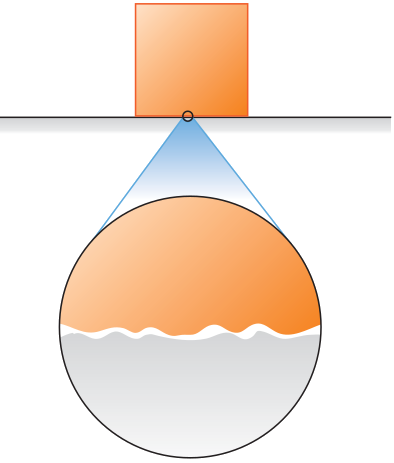
\includegraphics[scale=.3]{friction_block}};
	\node at (1,2) {\ak \text{វត្ថុ}};
	\node at (2.5,1) {\ak \text{ផ្ទៃប៉ះ}};
	\end{tikzpicture}
	\caption{កម្លាំងកកិត}
\end{figure}
\begin{exercise}
	\begin{enumerate}
		\item នៅលើផ្លូវដេកត្រង់មួយរថយន្តដែលមានម៉ាស $m=1$តោន បានចាប់ហ្រ្វាំងដើម្បីឈប់គោរពតាមស្លាកសញ្ញាចរាចរ។ កម្លាំងកកិត $2$ នៃប្រាំងទាំងអស់សមមូលនឹងកម្លាំងថេរតែមួយដែលមានទិសដេកមានទិសដៅផ្ទុយពីចលនារបស់រថយន្ត និងមានតម្លៃ $f=2000\si{\newton}$។ គណនាសំទុះនៃចលនារបស់រថយន្ត។
		\begin{figure}[H]
			\centering
			\begin{tikzpicture}
				\coordinate (O) at (0,0);
				\node at (0,0) {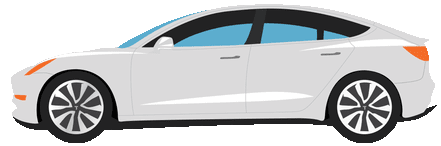
\includegraphics[scale=.2]{car_driving}};
				\fill[left color = white, right color=white, fill opacity=1, bottom color=gray, top color=gray!40!white] (-2,-.7) rectangle (2,-.5);
			\end{tikzpicture}
		\end{figure}
		\item រថយន្តមួយផ្លាស់ទីដោយល្បឿន $10\si{\metre/\second}$ លើផ្លូវដេកត្រង់រាបស្មើ។ ចាប់ពីពេលពន្លត់ម៉ាស៊ីនរហូតដល់ពេលឈប់ស្ងៀមរថយន្តរត់បានចម្ងាយ $150\si{\metre}$។ តើរថយន្តរត់លើចម្ងាយផ្លូវនេះក្នុងរយៈពេលប៉ុន្មាន? មេគុណកកិតប៉ុន្មាន?(គេមិនគិតកម្លាំងទប់នៃខ្យល់)។ គេឲ្យ $g=9.80\si{\metre/\second^{2}}$។
	\end{enumerate}
\end{exercise}
\section{អនុវត្តន៍ច្បាប់ញូតុន}
\quad នៅចំណុចនេះយើងនឹងសិក្សាអំពីការប្រើ ឬការអនុវត្តច្បាប់ទាំងបីរបស់ ញូតុន ដើម្បីធ្វើការដោះស្រាយលំហាត់ ក៏ដូចជាស្វែងយល់បន្ថែមអំពីបាតុភូតជាក់ស្តែងរបស់លំហាត់។
\subsection{របៀបប្រើច្បាប់ញូតុនដើម្បីដោះស្រាយលំហាត់}
\begin{key}
	ដើម្បីដោះស្រាយលំហាត់ទាក់ទងនិងច្បាប់ញូតុន យើងត្រូវ៖
	\begin{enumerate}
		\item វិភាគប្រធានលំហាត់ និងបាតុភូតរួចគូសរូប
		\item គូសដ្យាក្រាមកម្លាំងក្រៅទាំងអស់ដែលមានអំពើលើអង្គធាតុនីមួយៗ
		\item ទម្លាក់ចំណោលកែងកម្លាំងនីមួយៗលើអ័ក្ស $\left(\overrightarrow{ox}\right)$ និង $\left(\overrightarrow{oy}\right)$
		\item អនុវត្តច្បាប់ ញូតុន ទៅតាមសម្មតិកម្មដែលគេប្រាប់៖
		\begin{itemize}
			\item បើអង្គធាតុមានលំនឹង ឬមានចលនាត្រង់ស្មើៈ យើងត្រូវប្រើច្បាប់ទី១ ញូតុន ពោលគឺ ឲ្យផលបូកនៃវ៉ិចទ័រកម្លាំងទាំងអស់ដែលមានអំពើលើអង្គធាតុស្មើសូន្យ គេសរសេរ $\Sigma\vec{F}=\vec{0}$	
			\item បើអង្គធាតុផ្លាស់ទីដោយសំទុះថេរ ឬមានចលនាត្រង់ប្រែប្រួលស្មើ យើងត្រូវប្រើច្បាប់ទី២ ញូតុន ពោលគឺ ឲ្យផលបូកនៃវ៉ិចទ័រកម្លាំងទាំងអស់ដែលមានអំពើលើអង្គធាតុស្មើនឹង ម៉ាសគុណនឹងសំទុះរបស់វា គេសរសេរ $\Sigma \vec{F}=m\vec{a}$
		\end{itemize}
		\item សរសេរកន្សោមវ៉ិចទ័រខាងលើ ជាម៉ូឌុល
		\item បង្កើតជាសមីការ រួចដោះស្រាយសមីការនោះ ដើម្បីរកអញ្ញាតដែលគេចង់សួររក។
	\end{enumerate}
\end{key}
\subsection{អង្គធាតុរអិលលើប្លង់ទេរ}
\begin{example}
	\begin{enumerate}
		\item ធុងមួយមានម៉ាស $m$ ដាក់លើផ្ទៃរលោង(កកិតអាចចោលបាន)នៃប្លង់ទេ មួយដែលបង្កើតបានមុំ $\theta$ ជាមួយប្លង់ដេកដូចរូបខាងក្រោម។ ចូរសិក្សាចលនារបស់ធុងក្រោយពីវាត្រូវបានគេលែង។
		\item រូបខាងក្រោម មេគុណកកិតស៊ីនេទិចរវាងដុំម៉ាស $A$ នឹងតុស្មើ​ $0.2$។ ដុំម៉ាស $m_{A}=25\si{\kilogram}$ និង $m_{B}=15\si{\kilogram}$។ ម៉ាសខ្សែ ម៉ាសរ៉ក និងកកិតរវាងខ្សែនឹងរ៉កអាចចោលបាន។ សំទុះទំនាញដី $g=9.80\si{\metre/\second^{2}}$
		\begin{enumerate}[k,2]
			\item គូសដ្យាក្រាមកម្លាំងនៃដុំម៉ាសនីមួយៗ។
			\item រកសំទុះនៃដុំម៉ាសនីមួយៗ។
			\item រកតំណឹងខ្សែ។
			\item តើដុំម៉ាសនីមួយៗផ្លាស់ទីបានប្រវែងប៉ុន្មានក្នុងរយៈពេល $3\si{\second}$ ដំបូងក្រោយពេលលែងដុំម៉ាស$B$
		\end{enumerate}
	\end{enumerate}
	\begin{figure}[H]
		\centering
		\begin{subfigure}[b]{0.45\textwidth}
			\begin{tikzpicture}
				\begin{scope}
					\coordinate (A) at (0,2);
					\coordinate (B) at (4,0);
					\coordinate (C) at (0,0);
					\draw (A)--(B)--(C)--cycle;
					\pic [draw, -, "$\theta$", angle eccentricity=1.5, angle radius=1cm] {angle = A--B--C};
					\draw[gray!40!black, line width=2.5pt] (-.2,0)--(4.2,0);
					\fill[left color = white, right color=white, fill opacity=1, bottom color=gray!40!white, top color=gray] (-.2,0) rectangle (4.2,-.2);
					\draw[gray!40!black, fill=cadetgrey,rotate around={-26.5:(1,1.75)}] (0,2.18) rectangle (1,1.55);
					\draw[dashed, gray!40!black,pattern=north west lines,rotate around={-26.5:(1,1.75)}] (3.3,1.55) rectangle (4.3,2.2);
					\draw[|-|] (1.2,2)--(3.1,1);
					\draw[>=Stealth, ->, line width=2pt] (1.3,2.4) to (2,2) node[above] (2,2) {$\vec{a}$};
					\node at (2.5,1.8) {$d$};
				\end{scope}
			\end{tikzpicture}
			\caption{ធុងរអិលលើប្លង់ទេរ}
		\end{subfigure}
		\begin{subfigure}[b]{0.45\textwidth}
			\begin{tikzpicture}[decoration=rope]
				\coordinate (O) at (0,0);
				\node at (O) {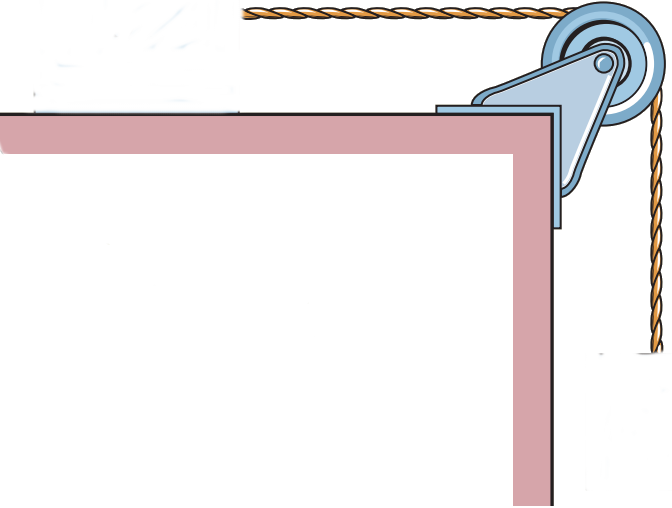
\includegraphics[scale=.18]{pulley_system}};
				\draw[fill=white] (0,1.5) circle (.15cm);
				\filldraw[gray!40!black,fill=cadetgrey] (-1.5,.9) rectangle (0,2.2);
				\node at (-.7,1.5) {$A$};
				\draw[fill=white] (2.05,0) circle (.15cm);
				\filldraw[gray!40!black,fill=cadetgrey] (1.6,-1) rectangle (2.5,0);
				\node at (2.05,-.5) {$B$};
				\draw[>=Stealth, ->, line width=2pt] (2.75, -.5) to (2.75, -1.5) node[right] (3, -1.5) {$\vec{a}$};
				\draw[>=Stealth, ->, line width=2pt] (.5, 1.75) to (1.5, 1.75) node[above] (2, 1.75) {$\vec{a}$};
			\end{tikzpicture}
			\caption{ប្រព័ន្ធរ៉ក}
		\end{subfigure}
	\end{figure}
\end{example}
\newpage
\subsection{ម៉ាស៊ីនអាត់វូត}
\begin{example}
	កាលណាវត្ថុពីរមានម៉ាសមិនស្មើគ្នាចងភ្ជាប់តាមរយៈខ្សែដែលឆ្លងកាត់រ៉ក។ កកិតរវាងរ៉ក និងខ្សែអាចចោលបាន។ ម៉ាសខ្សែ និងម៉ាសរ៉កអាចចោលបាន។ ប្រព័ន្ធដែលបានរៀបរាប់នេះហៅថា ម៉ាស៊ីនអាត់វូត។\\
 	កំណត់សំទុះវត្ថុទាំងពីរ និងតំណឹងខ្សែ។ ចូរអនុវត្តជាលេខបើ $m_{1}=1.0\si{\kilogram},~m_{2}=2.0\si{\kilogram}$ និង $g=9.80\si{\metre/\second^{2}}$។
	\begin{figure}[H]
		\centering
		\begin{tikzpicture}
		\coordinate (O) at (0,0);
		\node at (0,0) {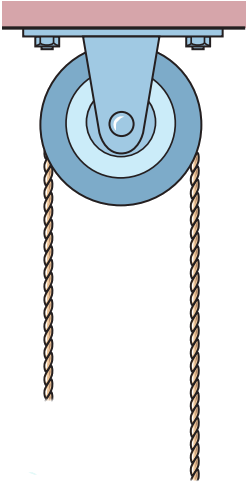
\includegraphics[scale=.25]{pulley}};
		\draw[fill=white] (.65,-2) circle (.15cm);
		\draw[fill=white] (-.65,-.5) circle (.15cm);
		\filldraw[gray!40!black,fill=cadetgrey] (-1.1,-1.5) rectangle (-.2,-.5);
		\filldraw[gray!40!black,fill=cadetgrey] (0,-2) rectangle (1.3,-3.3);
		\node at (-.65,-1) {$m_{1}$};
		\node at (.65,-2.7) {$m_{2}$};
		\draw[>=Stealth, ->, line width=2pt] (-1.7,-1) to (-1.7, .5) node[left] (-1.7, .5) {$\vec{a}$};;
		\draw[>=Stealth, ->, line width=2pt] (1.7, -2.7) to (1.7, -4) node[right] (1.7, -4) {$\vec{a}$};
		\end{tikzpicture}
		\caption{ម៉ាស៊ីនអាត់វូត}
	\end{figure}
\end{example}
\begin{exercise}
	\begin{enumerate}
		\item កម្លាំងពីរមានអំពើលើវត្ថុមួយមានម៉ាស $m=4.0\si{\kilogram}$។ បើ $F_{1}=20.0N$ និង $F_{2}=15.0N$។ ចូរគណនា៖
		\begin{enumerate}[k,2]
			\item កម្លាំងផ្គូបដែលមានអំពើលើវត្ថុនោះ។
			\item គណនាសំទុះនៃវត្ថុនោះ។
		\end{enumerate}
		\item ឈើមួយដុំរាងប្រលេពីប៉ែតកែងបានរអិលដោយគ្មានកកិតចុះតាមបណ្តោយប្លង់ទេ(ដូចរូប)។ មុំរវាងប្លង់ទេរ និងប្លង់ដេកគឺ $\theta=30^\circ$។ ដុំឈើនោះចាប់ផ្តើមផ្លាស់ទីពី $A$ ចុះក្រោមតាមបណ្តោយប្លង់ទេរបានប្រវែង $d=2.0\si{\metre}$។
		\begin{enumerate}
			\item គូសដ្យាក្រាមតាងឲ្យកម្លាំងដែលមានអំពើលើដុំថ្មនោះ។
			\item គណនាសំទុះនៃឈើនោះ។
			\item គណនាល្បឿននៅខណៈដែលដុំឈើនោះមកដល់ចំណុច $B$។ គេយក $g=9.80\si{\metre/\second^2}$។
		\end{enumerate}
	\item អេឡិចត្រុងមួយមានម៉ាស $9.11\times10^{-31}\si{\kilogram}$ ធ្វើចលនាត្រង់ដោយល្បឿនដើម $2.0\times10^{5}\si{\metre/\second}$ និងផ្លាស់ទីបាន $5.0\si{\centi\metre}$។ គេដឹងថាសំទុះនៃអេឡិចត្រុងថេរនិងល្បឿនស្រេចគឺ $6.0\times10^{5}\si{\metre/\second}$។
	\begin{enumerate}
		\item កំណត់កម្លាំងដែលមានអំពើលើអេឡិចត្រុង។
		\item ប្រៀបធៀបកម្លាំងនេះនឹងទម្ងន់របស់អេឡិចត្រុង។ គេឲ្យ $g=9.80\si{\metre/\second^{2}}$។
	\end{enumerate}
	\end{enumerate}
	\begin{figure}[H]
		\centering
		\begin{subfigure}[b]{0.3\textwidth}
			\centering
			\begin{tikzpicture}
			\begin{scope}
			\coordinate (O) at (0,0);
			\coordinate[label=above:{$\vec{F}_{1}$}] (F2) at (0,2);
			\coordinate[label=right:{$\vec{F}_{2}$}] (F1) at (2,0);
			\draw [->, line width =2pt] (O) -- (F1);
			\draw [->, line width =2pt] (O) -- (F2); 
			\shade [ball color=cyan!20!white] (O) circle [radius=10pt];
			\node at (O) {$m$};
			\pic [draw, "$90.0^\circ$", angle eccentricity=1.7, angle radius=.7cm] {angle= F1--O--F2};
			\end{scope}
			\end{tikzpicture}
			\caption{រូបលំហាត់ទី១}
		\end{subfigure}
		\begin{subfigure}[b]{0.3\textwidth}
			\centering
			\begin{tikzpicture}
				\begin{scope}
					\coordinate (O) at (0,0);
					\coordinate[label=right:$\vec{F}_{2}$] (F1) at (2,0);
					\coordinate[label=above:$\vec{F}_{1}$] (F2) at (2,2);
					\draw [->, line width =2pt] (O) -- (F1);
					\draw [->, line width =2pt] (O) -- (F2); 
					\shade [ball color=cyan!20!white] (O) circle [radius=10pt];
					\node at (O) {$m$};
					\pic [draw, "$60.0^\circ$", angle eccentricity=1.5, angle radius=1cm] {angle= F1--O--F2};
				\end{scope}
			\end{tikzpicture}
			\caption{រូបលំហាត់ទី១}
		\end{subfigure}
		\begin{subfigure}[b]{0.3\textwidth}
			\centering
			\begin{tikzpicture}
			\begin{scope}
			\coordinate (A) at (0,2);
			\coordinate[label=above right:$B$] (B) at (4,0);
			\coordinate (C) at (0,0);
			\draw (A)--(B)--(C)--cycle;
			\pic [draw, -, "$\theta$", angle eccentricity=1.5, angle radius=1cm] {angle = A--B--C};
			\draw[gray!40!black, line width=2.5pt] (-.2,0)--(4.2,0);
			\fill[left color = white, right color=white, fill opacity=1, bottom color=gray!40!white, top color=gray] (-.2,0) rectangle (4.2,-.2);
			\draw[gray!40!black, fill=cadetgrey,rotate around={-26.5:(1,1.75)}] (0,2.18) rectangle (1,1.55);
			\draw[|-|] (1.2,2)--(4,.6);
			\node at (1.3,2.4) {$A$};
			\node at (2.8,1.5) {$d$};
			\end{scope}
			\end{tikzpicture}
			\caption{រូបលំហាត់ទី២}
		\end{subfigure}
	\end{figure}
\end{exercise}
\section{សំណួរ និងលំហាត់អនុវត្ត}
\begin{enumerate}
	\item ចូរអនុវត្តច្បាប់ទី១ ទែម៉ូឌីណាមិចក្នុងលំនាំអាដ្យាបាទិច។
	\item ចូររៀបរាប់វគ្គទាំងបួននៃដំណើរការម៉ាសុីនម៉ាស៊ូត។
	\item ចូររៀបរាប់ដំណើរប្រព្រឹត្តទៅនៃសុិចកាកណូ។
	\item ដូចម្តេចដែលហៅថា ម៉ូទ័រចំហេះក្រៅ? ម៉ូទ័រចំហេះក្នុង?
	\item ធ្វើដូចម្តេចដើម្បីតម្លើងទិន្នផលម៉ាសុីនកម្តៅ?
	\item ម៉ាសុីនកាកណូ ៣ $\left(a,b,c\right)$ ដំណើរការចន្លោះសីតុណ្ហភាពៈ $(a) 400K$ និង $500K$ $\left(b\right) 500K$ និង $600K$ $\left(c\right) 400K$ និង $600K$។ ម៉ាសុីននីមួយៗស្រូបបរិមាណកម្តៅដូចៗគ្នាពីធុងក្តៅរាល់សុិច។ ចូររៀបតម្លៃកម្មន្តដែលធ្វើដោយម៉ាសុីនទាំងបីតាមលំដាប់ពីធំទៅតូច។
	\item តើប្រភពក្តៅ និងប្រភពត្រជាក់របស់ម៉ាសុីនសាំងបន្ទុះបួនវគ្គស្ថិតនៅត្រង់តំបន់ណា? ចូរពន្យល់?
	\item កម្មន្តដែលធ្វើលើឧស្ម័នក្នុងរយៈពេលនៃលំនាំអាដ្យបាទិចគឺ $140J$។ គណនាកំណើនថាមពលក្នុងនៃប្រព័ន្ធជាកាឡូរី។
	\item ម៉ាសុីនអុីដេអាល់មួយបានបំពេញកម្មន្ត $300J$។ យើងដឹងថាម៉ាសុីនបានបញ្ចេញកម្តៅទៅមជ្ឈដ្ឋានក្រៅ $600J$។ តើម៉ាសុីននោះមានទិន្នផលប៉ុន្មាន?
	\item ម៉ាសុីនកាកណូស្រូបកម្តៅ $1200cal$ ក្នុងរយៈពេលមួយសុិចនិងដំណើរការនៅចន្លោះសីតុណ្ហភាព $500K$ និង $300K$។
	\begin{enumerate}
		\item គណនាទិន្នផលនៃម៉ាសុីន។
		\item គណនាកម្តៅដែលម៉ាសុីនបានបញ្ចេញចោល។
		\item គណនាកម្មន្តដែលបានធ្វើក្នុងរយៈពេលមួយសិុចជាស៊ូល។
	\end{enumerate}
	\item ម៉ាសុីនកាកណូមានដំណើរការនៅចន្លោះសីតុណ្ហភាព $T_{h}=850K$ និង $T_{c}=300K$។ ក្នុងសុិចនីមួយៗម៉ាសុីនបានបំពេញកម្មន្ត $1200J$ ក្នុងរយៈពេល $0.25s$។
	\begin{enumerate}
		\item គណនាទិន្នផលនៃម៉ាសុិន។
		\item គណនាតម្លៃមធ្យមនៃអានុភាពរបស់ម៉ាសុីន។
		\item គណនាបរិមាណកម្តៅដែលផ្តល់ដោយធុងដែលមានសីតុណ្ហភាពខ្ពស់។
		\item គណនាបរិមាណកម្តៅដែលផ្តល់ដោយធុងដែលមានសីតុណ្ហភាពទាប។
	\end{enumerate}
	\item ម៉ូទ័រសាំងនៃរថយន្តរេណូល{\en(Renault)} បានទទួលកម្តៅ $2\times10^{5}J/s$ ដើម្បីឲ្យមានបន្ទុះក្នុងកាប៊ុយរ៉ង់។ វាបានបញ្ចេញកម្តៅ $1.3\times10^{5}J/s$ ទៅមជ្ឈដ្ឋានក្រៅ។
	\begin{enumerate}
		\item គណនាកម្មន្តដែលធ្វើដោយពិស្តុងក្នុងរយៈពេល $1$ វិនាទី។
		\item គណនាទិន្នផលកម្តៅនៃម៉ាសុីន។
		\item គេដឹងថាទិន្នផលមេកានិចគឺ $0.85$។ គណនាកម្មន្តដែលភ្លៅម៉័ទ័របានទទួលក្នុងរយៈពេល $1$ វិនាទី។
	\end{enumerate}  
	\item គណនាកម្មន្តអតិបរមាដែលម៉ាសុីនកាកណូមួយអាចបង្កើតឡើងពេលវាទទួលកម្តៅ $1kcal$ បើវាស្រូបកម្តៅនៅសីតុណ្ហភាព $427^\circ C$ និងបញ្ខេញនៅ $177^\circ C$។
	\item ម៉ាសុីនមួយបញ្ចេញកម្តៅ $8200J$ ខណៈពេលដែលម៉ាសុីនធ្វើកម្មន្តបាន $2600J$។ គណនាទិន្នផលនៃម៉ាសុីននេះ។
	\item ម៉ាសុីនកម្តៅមួយទទួលថាមពល $360J$ ពីធុងក្តៅ និងផ្តល់កម្មន្ត $25J$ ក្នុងវគ្គនីមួយៗ។
	\begin{enumerate}
		\item គណនាទិន្នផលនៃម៉ាសុីន។
		\item គណនាកម្តៅស្រូបដោយធុងត្រជាក់ក្នុងវដ្តនីមួយៗ
	\end{enumerate}
	\item ម៉ាសុីនមួយមានទិន្នផលកម្តៅ $30\%$។ គណនា៖
	\begin{enumerate}
		\item កម្មន្តដែលបានធ្វើ ប្រសិនបើវាស្រូបកម្តៅ $150J$ ពីធុងក្តៅ។
		\item កម្តៅភាយចេញទៅធុងត្រជាក់ក្នុងវដ្តនីមួយៗ។
	\end{enumerate}
	\item ម៉ាសុីនកាកណូធ្វើការរវាងធុងក្តៅពីរនៅសីតុណ្ហភាព $500K$ និង $300K$។ 
	\begin{enumerate}
		\item រកទិន្នផលកម្តៅនៃម៉ាសុីនកាកណូ។
		\item បើវាស្រូបកម្តៅ $200kJ$ ពីធុងក្តៅ។ គណនាកម្មន្តដែលបានធ្វើ។
	\end{enumerate}
	\item ម៉ាសុីនកម្តៅមយមានអានុភាព $580MW$។ គណនាកម្តៅដែលម៉ាសុីនបាត់បង់រាល់វិនាទី បើគេដឹងថាម់ាសុីនមានទិន្នផល $32\%$។
	\item ម៉ូទ័រម៉ាសុីនម៉ាស៊ូតនៃរថយន្តមួយដែលមានទិន្នផលកម្តៅ $0.43$ ហើយស្រូបកម្តៅ $4.0MJ$ ពីប្រភពក្តៅ។\\គណនាៈ
	\begin{enumerate}
		\item កម្មន្តមេកានិចដែលបានពីពិស្តុង។
		\item បរិមាណកម្តៅដែលបញ្ចេញទៅក្នុងបរិយាកាស។
		\item កម្មន្តបានការ បើគេដឹងថាទិន្នផលគ្រឿងបញ្ចូន $0.82$។
	\end{enumerate} 
	\item ម៉ាសុីនកាកណូដែលមានអានុភាព $500W$ ដំណើរការចន្លោះសីតុណ្ហភាព $100^\circ C$ និង $60^\circ C$។ 
	\begin{enumerate}
		\item គណនាថាមពលកម្តៅស្រូបដោយម៉ាសុីនរាល់វិនាទី។
		\item គណនាកម្តៅបញ្ចេញដោយម៉ាសុីនរាល់វិនាទី។
	\end{enumerate}
	\item ម៉ាសុីនកាកណូដំណើរការនៅចន្លោះធុងកម្តៅពីរដែលមានសីតុណ្ហភាព $235^\circ C$ និង $115^\circ C$ ដោយស្រូបកម្តៅ $6.30\times10^{4}J$ រាល់វដ្តពីធុងក្តៅ។
	\begin{enumerate}
		\item គណនាទិន្នផលនៃម៉ាសុីន។
		\item គណនាកម្មន្តដែលម៉ាសុីនបានបំពេញ។
	\end{enumerate}
	\item ម៉ាសុីនម៉ាស៊ូតនៃរថយន្តមួយមានទិន្នផលកម្តៅ $0.40$ ហើយវាស្រូបបរិមាណកម្តៅ $6.0\times10^{6}J$។ គណនាៈ
	\begin{enumerate}
		\item កម្មន្តមេកានិចដែលបានពីពិស្តុង។
		\item បរិមាណកម្តៅដែលបញ្ចេញទៅក្នុងបរិយាកាស។
		\item កម្មន្តបានការ បើទិន្នផលគ្រឿងបញ្ជូនស្មើនឹង $0.8$។
	\end{enumerate}
	\item ម៉ាសុីនអុីដេអាល់មួយដំណើរការនៅចន្លោះធុងកម្តៅពីរដែលមានសីតុណ្ហភាព $500K$ និង $400K$ វាស្រូបកម្តៅ $10.0\times10^{2}J$ ពីធុងដែលមានសីតុណ្ហភាពខ្ពស់ក្នុងរយៈពេលសិុចនីមួយៗ។
	\begin{enumerate}
		\item គណនាទិន្នផលរបស់ម៉ាសុីននោះ។
		\item តើកម្តៅដែលម៉ាសុីនបញ្ចេញទៅមជ្ឈដ្ឋានក្រៅមានតម្លៃប៉ុន្មាន?
	\end{enumerate}
	\item កម្មន្តដែលបំពេញដោយម៉ាសុីនមួយស្មើនឹង $1/4$ នៃកម្តៅស្រូបពីធុងក្តៅ។
	\begin{enumerate}
		\item គណនាទិន្នផលអតិបរមានៃម៉ាសុីន។
		\item តើម៉ាសុីនខាតបង់កម្តៅប៉ុន្មានភាគរយ។
	\end{enumerate}
	\item ម៉ូទ័រម៉ាស៊ូតមួយទទួើលកម្តៅ $3.83MJ$។ វាមានទិន្នផលកម្តៅ $0.45$។
	\begin{enumerate}
		\item គណនាកម្មន្តមេកានិចដែលផ្តល់ដោយពិស្តុង។
		\item តើកម្តៅដែលបញ្ចេញទៅក្នុងបរិយាកាសមានតម្លៃប៉ុន្មាន?
		\item ទិន្នផលគ្រឿងបញ្ចូនគឺ $0.85$។
			  គណនាកម្មន្តដែលបញ្ចូនដោយភ្លៅម៉ូទ័រ។
	\end{enumerate}
	\item ម៉ាសុីនកម្តៅមួយមានអានុភាពចេញ $5.00kW$ និងមានទិន្នផល $25\%$។ ម៉ាសុីនបានបំភាយកម្តៅ $8.00\times10^{3}J$ រាល់វដ្តនីមួយៗ។
	\begin{enumerate}
		\item គណនាកម្តៅស្រូបដោយម៉ាសុីនរាល់វដ្តនីមួយៗ។
		\item គណនារយៈពេលក្នុងមួយវដ្តនៃដំណើរការ។
	\end{enumerate}
	\item ម៉ាសុីនកម្តៅមួយស្រូបកម្តៅ $360J$ ពីធុងក្តៅ និងបំពេញកម្មន្ត $25.0J$ ក្នុងវដ្តនីមួយៗ។
	\begin{enumerate}
		\item គណនាទិន្នផលនៃម៉ាសុីន។
		\item គណនាកម្តៅភាយទៅធុងត្រជាក់។
	\end{enumerate}
	\item សីតុណ្ហភាពនៅក្នុងធុងត្រជាក់នៃម៉ាសុីនកាណូគឺ $230^\circ C$។ គណនាសីតុណ្ហភាពនៅក្នុងធុងក្តៅ បើម៉ាសុីនមានទិន្នផល $34\%$។
	\item ម៉ាសុីនកាណូមួយដំណើរការចន្លោះសីតុណ្ហភាព $210^\circ C$ និង $45^\circ C$។ អានុភាពចេញរបស់វាគឺ $910W$។\\ គណនាកម្តៅភាយចេញពីម៉ាសុីនរាល់វិនាទី។
	\item ម៉ាសុីនកាណូមួយមានទិន្នផល $22\%$។ វាដំណើរការចន្លោះធុងកម្តៅពីរដែលមានបម្រែបម្រួលសីតុណ្ហភាព $75.0^\circ C$។
	\begin{enumerate}
		\item គណនាសីតុណ្ហភាពក្នុងធុងក្តៅ។
		\item គណនាសីតុណ្ហភាពក្នុងធុងត្រជាក់។
	\end{enumerate}
	\item ម៉ាសុីនកាកណូមួយមានអានុភាព $520kW$ ដោយស្រូបកម្តៅ $950kcal$ រាល់វិនាទី។ ប្រសិនបើសីតុណ្ហភាពប្រភពក្តៅ $520^\circ C$ ចូរគណនាសីតុណ្ហភាពប្រភពត្រជាក់។
	\item ម៉ាសុីនសាំងមួយដែលមានសុីឡាំងចំនួនបួនមានទិន្នផល $0.22$ និងបំពេញកម្មន្តបាន $180J$ រាល់ជុំក្នុងសុីឡាំងនីមួយៗ។ ប្រសិនបើម៉ាសុីនដំណើរការបាន $25\mathbf{rps}$។
	\begin{enumerate}
		\item គណនាកម្មន្តបំពេញក្នុងមួយវិនាទី។
		\item គណនាកម្តៅសរុបដែលផ្តលឲ្យម៉ាសុីនក្នុងមួយវិនាទី។
		\item ប្រសិនបើចំហេះសាំង $1\ell$ ផ្តល់ថាមពលបាន $32.21MJ$។\\ តើក្នុងសាំងមួយលីត្រអាចប្រើបានក្នុងរយៈពេលប៉ុន្មាន។
	\end{enumerate}
	\item ម៉ាសុីនកម្តៅទី $1$ ទទួលកម្តៅធំជាងម៉ាសុីនទី $2$ បួនដង បានបំពេញកម្មន្តពីរដង និងបញ្ចេញកម្តៅប្រាំពីរដងនៃម៉ាសុីនទី $2$ ទៅធុងត្រជាក់វិញ។ គណនាទិន្នផលនៃម៉ាសុីនទាំងពីរ។
	\item ម៉ាសុីនកាណូមួយដំណើរការចន្លោះសីតុណ្ហភាព $293K$ និង $67K$។ តើវិធីសាស្រ្តណាមួយដែលធ្វើឲ្យទិន្នផលនៃម៉ាសុីនកើនឡើងខ្ពស់ជាង "បង្កើនសីតុណ្ហភាព $10^\circ C$ នៅក្នុងធុងក្តៅ" ឬក៏ "បន្ថយសីតុណ្ហភាព $10^\circ C$ នៅក្នុងធុងត្រជាក់"? ចូរបង្ហាញហេតុផលសាមញ្ញមួយ។
	\item ម៉ាសុីនកម្តៅបញ្ចេញកម្តៅទៅកាន់ធុងដែលមានសីតុណ្ហភាព $340^\circ C$ និងមានទិន្នផលទ្រឹស្តី $36\%$។ តើធុងត្រជាក់មានសីតុណ្ហភាពប៉ុន្មានអង្សា ប្រសិនបើម៉ាសីុនកើនទិន្នផលដល់ $42\%$ និងរក្សាសីតុណ្ហភាពក្នុងប្រភពក្តៅដដែល។
	\item ម៉ាសុីនកាណូមួយដំណើរការចន្លោះប្រភពកម្តៅដែលមានសីតុណ្ហភាព $580^\circ C$ និងមានទិន្នផលអតិបរមា $22\%$។ ដើម្បីបង្កើនទិន្នផលម៉ាសុីនដល់ $42\%$ តើគេត្រូវតម្លើងសីតុណ្ហភាពប្រភពក្តៅដល់ប៉ុន្មានអង្សា បើសីតុណ្ហភាពប្រភពត្រជាក់ត្រូវរក្សា?
	\item ម៉ាសុីនកាណូមួយមានធុងត្រជាក់ដែលមានសីតុណ្ហភាព $17^\circ C$ មានទិន្នផល $40\%$។ តើគេត្រូវតម្លើងសីតុណ្ហភាព ប្រភពក្តៅប៉ុន្មានដើម្បឲ្យទិន្នផលរបស់ម៉ាសុីនកើនដល់ $50\%$។\\ ដោយដឹងថាសីតុណ្ហភាពប្រភពត្រជាក់ត្រូវបានរក្សា។
	\item ម៉ាសុីនកាណូមួយប្រើចំហាយទឹកក្តៅ $100^\circ C$ ដែលជាធុងក្តៅ។ រីឯធុងត្រជាក់គឺជាមជ្ឈដ្ឋានខាងក្រៅ ដែលមានសីតុណ្ហភាព $20^\circ C$។ អត្រាថាមពលដែលត្រូវបានបញ្ចូនទៅកាន់ធុងត្រជាក់មាន $15.4W$។
	\begin{enumerate}
		\item គណនាអានុភាពបានការនៃម៉ាសុីនកម្តៅ។
		\item គណនាចំហាយកំណជាទឹកនៅធុងក្តៅក្នុងរយៈពេល $1.00h$ ហើយកម្តៅឡាតង់ដើម្បីឲ្យចំហាយកំណជាទឺក $L=2.26\times10^{6}J/kg$។
	\end{enumerate}
	\item ម៉ាសុីនកម្តៅមួយ ត្រូវបានតភ្ជាប់ទៅធុងកម្តៅពីរដែលមួយជាអាលុយមីញ៉ូមរលាយនៅសីតុណ្ហភាព $660^\circ C$ និងធុងមួយទៀត គឺដុំបារតនៅសីតុណ្ហភាព $-38.9^\circ C$។ ម៉ាសុីនដំណើរការដោយបង្កកអាលុយមីញ៉ូម $1.0g$ និងរំលាយបារត $15.0g$។ គេដឹងថា បន្សាយកម្តៅម៉ាសអាលុយមីញ៉ូម $3.97\times10^{5}J/kg$ និងបន្សោយកម្តៅម៉ាសបារត $1.18\times10^{4}J/kg$។ គណនាទិន្នផលអតិបរមានៃម៉ាសុីន។
	\item ម៉ាសុីនកាណូប្រើចំហាយទឹកមួយចាប់ផ្តើមដំណើរការរវាងសីតុណ្ហភាពចំហាយ $220^\circ C$ និងសីតុណ្ហភាព $35^\circ C$ ដោយផ្តល់នូវអានុភាព $8hp$(សេះ)។ គណនាកម្តៅស្រូបក្នុងមួយវិនាទីដោយម៉ាសុីនចំហាយ និងកម្តៅបញ្ចេញក្នុងមួយវិនាទីគិតជាកាឡូរី។ បើម៉ាសុីនកាណូដំណើរការរវាងសីតុណ្ហភាពកម្រិតទាំងនេះមានទិន្នផល $30\%$ នៃទិន្នផលកម្តៅ។
	\newpage
	\item ម៉ាសុីន $X$ បានទទួលថាមពលកម្តៅពីធុងដែលមានសីតុណ្ហភាពខ្ពស់ $4$ដងធំ ជាងម៉ាសុីន $Y$។ ម៉ាសុីន $X$ បានធ្វើកម្មន្ត $2$ដង ហើយបានបញ្ចេញថាមពលកម្តៅ $7$ដងដោយធុងដែលមានសីតុណ្ហភាពទាបធំជាងម៉ាសុីន $Y$។
	\begin{enumerate}
		\item គណនាទិន្នផលម៉ាសុីនកម្តៅ $Y$។
		\item គណនាទិន្នផលម៉ាសុីនកម្តៅ $X$។
	\end{enumerate}
	\item សុីឡាំងច្រើនរបស់ម៉ាសុីនសាំងយន្នហោះមួយដំណើរការដោយល្បឿន $2500\mathbf{tr/mn}$ ដោយទទួលថាមពលកម្តៅ $7.89\times10^{3}J$ និងបញ្ចេញថាមពលកម្តៅ $4.58\times10^{3}J$ ក្នុងជុំនីមួយៗនៃម៉ាសុីនយន្នហោះវីឡឺ​​​ប្រឺ​​កាំង។
	\begin{enumerate}
		\item គណនាប្រេងសាំងគិតជាលីត្រក្នុងរយៈពេល $1$ម៉ោងនៃដំណើរការ។\\ ប្រសិនបើកម្តៅចំហេះនៃសាំង $4.03\times10^{7}J/L$។
		\item គណនាអានុភាពមេកានិចដែលម៉ាសុីនផលិតបាន។
		\item គណនាម៉ូម៉ង់ដែលម៉ាសុីនយន្តហោះប្រើលើបន្ទុក។
		\item គណនាអានុភាពមិនបានការដែលបានបញ្ចេញដោយធុងសីតុណ្ហភាពទាប។
	\end{enumerate}
	\item ម៉ាសុីនកាណូមួយផលិតអានុភាពបានការ $150kW$។ ម៉ាសុីននេះបានដំណើរការរវាងសីតុណ្ហភាពពីរគឺ $20^\circ C$ និង $500^\circ C$។
	\begin{enumerate}
		\item គណនាថាមពលជាកម្តៅដែលវាទទួលបានក្នុងរយៈពេល $1$ម៉ោង។
		\item គណនាថាមពលជាកម្តៅដែលវាបាត់បង់ក្នុងរយៈពេល $1$ម៉ោង។
	\end{enumerate}
	\item ម៉ាសុីនកាណូមួយមានអានុភាព $P$។ ម៉ាសុីននេះបានដំណើរការរវាងដំណើរការរវាងសីតុណ្ហភាពពីរគឺ $T_{h}$ និង $T_{c}$។
	\begin{enumerate}
		\item គណនាថាមពលជាកម្តៅដែលចូលក្នុងម៉ាសុីននៅចន្លោះពេល $\Delta t$។
		\item គណនាថាមពលជាកម្តៅដែលបាត់ប៉ង់ក្នុងចន្លោះពេល $\Delta t$។
	\end{enumerate}
	\item ម៉ាសុីនមួយបានបញ្ចូនថាមពលជាកម្តៅ $2\times10^{3}J$ ពីប្រភពធុងសីតុណ្ហភាពខ្ពស់ក្នុងអំឡុងខួបនីមួយៗហើយបានបញ្ចូន $1.5\times10^{3}J$ ទៅប្រភពសីតុណ្ហភាពទាប។
	\begin{enumerate}
		\item គណនាទិន្នផលរបស់ម៉ាសុីន។
		\item គណនាកម្មន្តដែលធ្វើដោយម៉ាសុីនក្នុង $1$ខួប។
		\item គេដឹងថា ម៉ាសុីននេះដំណើរការដោយល្បឿន $2000\mathbf{tr/mn}$។\\
		គណនាអានុភាពមេកានិចដែលម៉ាសុីននោះផលិតបានក្នុង $1$ជុំ។
	\end{enumerate}
	\item កម្មន្តដែលធ្វើដោយម៉ាសុីនស្មើ $1/4$ នៃថាមពលកម្តៅដែលស្រូបចេញពីធុងសីតុណ្ហភាពខ្ពស់។
	\begin{enumerate}
		\item គណនាទិន្នផលកម្តៅរបស់ម៉ាសុីន។
		\item គណនាផលធៀបថាមពលដែលស្រូបនិងថាមពលដែលបញ្ចេញទៅធុងសីតុណ្ហភាពទាប។
	\end{enumerate}
	\item កាំភ្លើងមយយត្រូវបានចាត់ទុកជាម៉ាសុីនកម្តៅ។ គេដឹងថាកាំភ្លើងធ្វើពីដែកដែលមានម៉ាសស្មើ $1.8kg$។ គ្រាប់កាំភ្លើងនេះមានម៉ាស $2.40g$ ហើយពេលបាញ់ចេញមានល្បឿន $320m/s$ និងមានទិន្នផលថាមពលស្មើ $1.10\%$។ សន្មតថាតួ(ដង)កំាភ្លើងស្រូបថាមពលទាំងអស់ដែលបញ្ចេញនិងកើនឡើងសីតុណ្ហភាពស្មើសាច់ក្នុងរយៈពេលខ្លឺមុនពេលបាត់បង់ថាមពលកម្តៅខ្លះទៅក្នុងមជ្ឈដ្ឋានបរិយាកាស។\\ គណនាកំណើនសីតុណ្ហភាពនៅក្នុងគ្រាប់កាំភ្លើង។ គេឲ្យកម្តៅម៉ាសដែក $C_{\text{ដែក}=448J/kg\cdot C^{\circ}}$។
	\item ម៉ាសុីនមួយកើតឡើងពីចំហេះធ្យូងថ្មបង្វិលតួប៊ីននៅជ្រលងស្ទឹង(អូហាយអូ) នៅសហរដ្ឋអាមេរិចដែលដំណើរការរវាងសីតុណ្ហភាពពីរ $1870^\circ C$ និង $430^\circ C$។
	\begin{enumerate}
		\item តើទិន្នផលម៉ាសុីនទ្រឹស្តីអតិបរមាស្មើប៉ុន្មាន?
		\item ទិន្នផលម៉ាសុីនពិតស្មើ $42\%$។ គណនាអនុភាពមេកានិចដែលម៉ាសុីនបានបញ្ចូន ប្រសិនវាស្រូបថាមពលកម្តៅ $1.40\times10^{5}J$ រៀងរាល់វិនាទីពីធុងសីតុណ្ហភាពខ្ពស់។
	\end{enumerate}
	\item ម៉ាសុីនកម្តៅមយយបង្កើតឡើងមានទិន្នផលស្មើម៉ាសុីនកាណូ $65\%$ នៅពេលវាដំណើរការរវាងធុងសីតុណ្ហភាពពីរ។
	\begin{enumerate}
		\item ប្រសិនបើសីតុណ្ហភាពធុងត្រជាក់ស្មើនឹង $20^\circ C$ តើសីតុណ្ហភាពដែលនៅធុងដែលមានសីតុណ្ហភាពខ្ពស់ស្មើប៉ុន្មាន?
		\item តើទិន្នផលម៉ាសុីនពិតអាចស្មើ $65\%$ ដែរឬទេ? ចូរពន្យល់?
	\end{enumerate}
	\item ក្នុងភាពទី១នៃភាពពីររបស់ម៉ាសុីនកាណូមួយថាមពលដែលស្រូប $Q_{1}$ ក្រោមសីតុណ្ហភាព $T_{1}$ ហើយធ្វើកម្មន្ត $W_{1}$ និងបញ្ចេញថាមពលកម្តៅ $Q_{2}$ ក្រោមសីតុណ្ហភាពទាប $T_{2}$។ ភាពទី២ ស្រូបថាមពលកម្តៅ $Q_{2}$ ធ្វើកម្មន្ត $W_{2}$ ហើយបញ្ចេញថាមពលកម្តៅ $Q_{3}$ ក្រោមសីតុណ្ហភាព $T_{3}$។\\
	ចូរបង្ហាញថា ទិន្នផលរបស់ម៉ាសុីនកម្តៅនេះគឺ $e=\frac{T_{1}-T_{3}}{T_{1}}=1-\frac{T_{3}}{T_{1}}$។ 
	\item ទិន្នផលនៃម៉ាសុីនពិត $20\%$ គឺប្រើដើម្បីបង្កើនល្បឿនរបស់រថភ្លើងមួយចេញពីស្ងៀមទៅល្បឿនប្រហែល $5m/s$។ យើងដឹងដា ម៉ាសុីនកាណូមួយបានប្រើប្រភពធុងត្រជាក់និងធុងក្តៅដូចគ្នាដើម្បីពន្លឿនរថភ្លើងដូចគ្នាពីនៅស្ងៀមទៅល្បឿន $6.50m/s$ ដោយប្រើបរិមាណបេ្រងឥន្ធនៈស្មើគ្នា។ ម៉ាសុីននេះប្រើខ្យល់ដែលមានសីតុណ្ហភាព $300K$ ធ្វើជាប្រភពធុងត្រជាក់។\\
	គណនាសីតុណ្ហភាពនៃចំហាយដែលប្រើនៅប្រភពធុងក្តៅ។
	\item ក្នុងមួយខួប ម៉ាសុីនកម្តៅមួយបានស្រូប $500J$ ពីធុងដែលមានសីតុណ្ហភាពខ្ពស់ហើយបញ្ចេញ $300J$ ទៅប្រភពធុងសីតុណ្ហភាពទាប។ គេដឹងថាទិន្នផលម៉ាសុីនស្មើនឹង $60\%$ នៃម៉ាសុីនកាណូ។ គណនាផលធៀបសីតុណ្ហភាពធុងត្រជាក់ និងសីតុណ្ហភាពធុងក្តៅនៃម៉ាសុីនកាណូ។
	\item ម៉ាសុីនកាណូមួយបានដំណើរការរវាងសីតុណ្ហភាព $T_{h}=100^\circ C$ និង $T_{c}=20^\circ C$។ តើផលធៀបទិន្នផលនៃម៉ាសុីនកាណូនេះកើនឡើងស្មើនឹងប៉ុន្មាន? បើសីតុណ្ហភាពធុងក្តៅកើនឡើងដល់ $550^\circ C$។
	\item $1500kW$ នៃម៉ាសុីនកម្តៅមួយបានដំណើរការដោយទិន្នផល $20\%$។ ថាមពលកម្តៅបានបញ្ចេញទៅធុងត្រជាក់ដោយការស្រូបចំហាយទឹកចូលក្នុងរបុំមានសិតុណ្ហភាព $20\%$។ ប្រសិនបើទឹក $60$លីត បានហូរឆ្លងកាត់របុំក្នុង១វិនាទី។ តើកំណើនសីតុណ្ហភាពទឹកស្មើនឹងប៉ុន្មាន? \\គេឲ្យកម្តៅម៉ាសទឹក $C=4186J/kg^\circ C$។ ម៉ាសមាឌទឹក $\rho=10^{3}kg/m^{3}$។
	\item ម៉ាសុីនកាណូមួយបានដំណើរការរវាងសីតុណ្ហភាពពីរគឺ $100^\circ C$ និង $20^\circ C$។
	គណនាម់ាសទឹកកកដែលអាចឲ្យម៉ាសុីនរំលាយបន្ទាប់ពីវាធ្វើកម្មន្ត $5\times10^{4}J$។ គេឲ្យកម្តៅឡាតង់របស់ទឹកកក $L_{f}=3.33\times10^{5}J/kg$
	\item ម៉ាសុីនកាណូមួយមានសីតុណ្ហភាពធុងត្រជាក់ $17^\circ C$ និងមានទិន្នផល $40^\circ C$។ តើសីតុណ្ហភាពធុងក្តៅកើនប៉ុន្មានដើម្បីឲ្យបានទិន្នផលរបស់ម៉ាសុីនកើនបាន $50\%$?
	\item ម៉ាសុីនកាណូមួយបានស្រូបថាមពលកម្តៅ $52kJ$ ហើយបានបញ្ចេញថាមពលកម្តៅ $36kJ$ ក្នុងខួបនីមួយៗ។
	\begin{enumerate}
		\item គណនាទិន្នផលរបស់ម៉ាសុីនកាណូ។
		\item គណនាកម្មន្តដែលបំពេញបានក្នុងខួបនីមួយៗ។
	\end{enumerate}
\end{enumerate}
\chapter{គោលការណ៍រលកតម្រួត និងរលកជញ្ជ្រុំ}
\section{ខួប និងប្រេកង់រលក}
\begin{definition}
	\begin{enumerate}[k]
		\item \emph{\kml ខួប} គឺជារយៈពេលដែលចល័ត ឬភាគល្អិតធ្វើឡើងច្រំដែលៗ។ ខួបរបស់រលកតាងដោយ $T$។
		\item \emph{\kml ប្រេកង់} គឺជាចំនួនលំយោលពេញដែលចល័តឬភាគល្អិតធ្វើបានក្នុង១វិនាទី។ ប្រេកង់តាងដោយ $f$ គិតជាអ៊ែក ឬក្នុង១វិនាទី $\left(Hz~;~1/s\right)$។
	\end{enumerate}
\end{definition}
	\begin{remark}
		\begin{enumerate}
			\item \emph{\kml ខួប} $T=\frac{1}{f}$
			\item \emph{\kml ប្រេកង់} $f=\frac{1}{T}$
			\item \emph{\kml ពុលសា​​ស្យុ​​ង ឬល្បឿនមុំ} $\omega = 2\pi f=\frac{2\pi}{T}$
		\end{enumerate}		
	\end{remark}
\begin{center}
	{\Large \kml\color{magenta} ចប់ដោយសង្ខេប!!!}
\end{center}
%
\includepdf{covers/back-cover.pdf}
\end{document}